\documentclass[11pt]{article}

\usepackage{latexsym}
\usepackage{algorithm,algpseudocode}
\usepackage{amsmath}
\usepackage{amssymb}
\usepackage{amsthm}
\usepackage{graphicx}
\usepackage{float}
\usepackage{wrapfig}
\usepackage{pseudocode}
\usepackage{subfigure}
\usepackage{url}
\usepackage[backref, colorlinks=true, citecolor=red, urlcolor=blue, pdfauthor={Jyh-Ming Lien}]{hyperref}


\newcommand{\handout}[5]{
  \noindent
  \begin{center}
  \framebox{
    \vbox{
      \hbox to 5.78in { {\bf } \hfill #2 }
      \vspace{4mm}
      \hbox to 5.78in { {\Large \hfill #5  \hfill} }
      \vspace{2mm}
      \hbox to 5.78in { {\em #3 \hfill #4} }
    }
  }
  \end{center}
  \vspace*{4mm}
}

\newcommand{\lecture}[4]{\handout{#1}{#2}{#3}{#4}{#1}}

\newtheorem{theorem}{Theorem}
\newtheorem{corollary}[theorem]{Corollary}
\newtheorem{lemma}[theorem]{Lemma}
\newtheorem{observation}[theorem]{Observation}
\newtheorem{proposition}[theorem]{Proposition}
\newtheorem{definition}[theorem]{Definition}
\newtheorem{claim}[theorem]{Claim}
\newtheorem{fact}[theorem]{Fact}
\newtheorem{assumption}[theorem]{Assumption}

% 1-inch margins, from fullpage.sty by H.Partl, Version 2, Dec. 15, 1988.
\topmargin 0pt
\advance \topmargin by -\headheight
\advance \topmargin by -\headsep
\textheight 8.9in
\oddsidemargin 0pt
\evensidemargin \oddsidemargin
\marginparwidth 0.5in
\textwidth 6.5in

\parindent 0in
\parskip 1.5ex
%\renewcommand{\baselinestretch}{1.25}

\begin{document}

\lecture{Midterm Exam Report}{Fall 2015}{Yeojin Kim}{Advance Algorithm Programming}
%%%%%%%%%%%%%%%%%%%%%%%%%%%%%%%%%%%%%%%%%%%%%%%%%%%%%%%%%%%%%%%%%%%%%%%%%%%%%%%%%%%%%%%%%%%%%%%%%%%%%%%%%%%%
\section{Summary of the two methods}
Hedcuter method and voronoi method consists of two steps : constructing weighted voronoi diagram and creating disks(i.e. stippling).
In case of constructing weighted voronoi diagram, initially both methods sample points in image pixels. Next, methods computes weighted voronoi diagram with given points using different approaches and move the points to new sites repeatedly.
For both cases, basically the centroid of a region is defined as
\begin{equation}\label{eq:centroid}
\mathbf{C_i}=\frac{\int_{A}\mathbf{x}\rho(\mathbf{x})dA}{\int_{A}\rho(\mathbf{x})dA}.
\end{equation}
%%%%%%%%%%%%%%%%%%%%%%%%%%%%%%%%%%%%%%%%%%%%%%%%%%%%%%%%%%%%%%%%%%%%%%%%%%%%%%%%%%%%%%%%%%%%%%%%%%%%%%%%%%%%
\subsection{hedcuter method}
The idea of fast stippling\cite{secord02} is mat the pixel to the stipple level  and copy stipples in it while looping through pixels.
For implementation, using the face that the two dimensional discrete function $f(x,y)$ of gray scale corresponds to the stipple level, it gathered the stipples looping through the site and propagating through the pixels.
The step is as below: 
\begin{enumerate}
\item Sample initial points $X=\{\mathbf{x_1, x_2, x_3, \cdots, x_n}\}$
\item Loop while the displacements don't exceed maximum site displacement and the number of iterations doesn't exceed maximum number of iterations,
\begin{enumerate}
\item Map the image value at $\mathbf{x_i}$ to stipple level $t_{\mathbf{x_i}}$
\item Propagate the stipple level at $\mathbf{x_i}$ to its neighbor
\item Compute the centroids $\mathbf{C_i}$
\item Move each points $\mathbf{x_i}$ to its new centers of a cell $\mathbf{C_i}$
\end{enumerate}
\item Create disks
\end{enumerate}
%Sampling
First of all, hedcuter samples a uniformly distributed random point for whole area of given image and test if this random point has high probability based on gaussian distribution. If that is the case, the algorithm keeps this point as an initial point and this process is repeated until generating $n$ points.
%Loop
In the loop, the algorithm keeps mapping image using the location of a point(which corresponds to the coordinates of a pixel) as unique identification. This mapping image contains the two dimensional discrete function $f(x,y)$ which also can corresponds to stipple level $t$ at each points with the number of levels $l$. Hedcuter method first computes and stores stipple level $t$ only at given points using Eq. \ref{eq:distance}.
\begin{equation}\label{eq:distance}
t_{\mathbf{x}}=l-I(\mathbf{x})
\end{equation}
Next, it sorts the stipples with stipple level, $x$ values, and $y$ values in ascending order.
Stipple level has a highest priority and $y$ values has a lowest priority in sorting.
Starting from a stipple which has the lowest stipple level, check the neighbors of the stipple.
A stipple level $t_{new}$ of a neighbor $nb$ can be newly computed from the current stipple $c$ based on Eq. \ref{eq:neigborDistance}.
\begin{equation}\label{eq:neigborDistance}
t_{new}=t_{c} + t_{nb}
\end{equation}
In case that a neighbor has a lower stipple level than stipple level it already has, hedcuter method keeps new stipple level and add this neighbor as stipple.After propagation of stipple level through all pixels, hedcuter method collect pixels which is affected by given points, so called coverage of a site. When computing the new center of a stipple, it compute weighted average of stipple levels in coverage.
%Creating disks 
At last, hedcuter method generates disks with sites information from the loop. The radius of disk is determined by intensity and user-specified disk size. The size of disks is inversely proportional to intensity of the sites. 

%%%%%%%%%%%%%%%%%%%%%%%%%%%%%%%%%%%%%%%%%%%%%%%%%%%%%%%%%%%%%%%%%%%%%%%%%%%%%%%%%%%%%%%%%%%%%%%%%%%%%%%%%%%%
\subsection{voronoi method}
A flow of voronoi method basically follows Lloyd's method\cite{Okabe:1992:STC:135734}, which as follows : \\
\begin{algorithm}
\caption{Lloyd's method}\label{alg:lloyds}
\begin{algorithmic}[1]
\While {generating point $\mathbf{x_i}$ not converged to centroids}
    \State Compute the Voronoi diagram of $\mathbf{x_i}$
    \State Compute the centroids $\mathbf{C_i}$ using equation (\ref{eq:centroid})
    \State Move each generating point $\mathbf{x_i}$ to its centroids $\mathbf{C_i}$
\EndWhile
\end{algorithmic}
\end{algorithm}\\
First, voronoi method samples points on the image randomly(Fig. \ref{fig:samples}) using Mersenne twister. 
\begin{figure*}[thb]
 \centering
 \subfigure[]{
    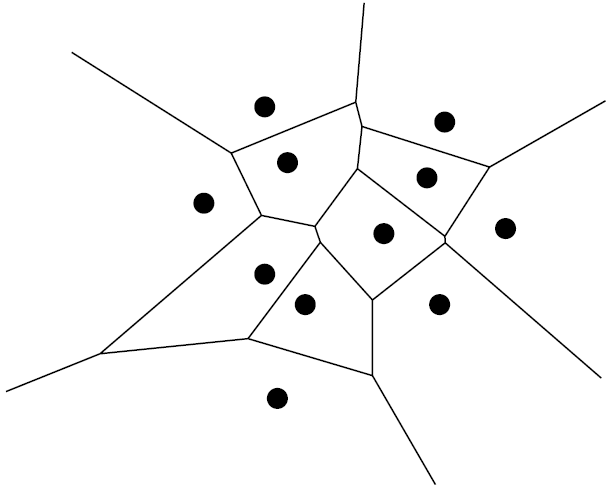
\includegraphics[width=0.32\textwidth]{FIGS/voronoi.png}
    \label{fig:voronoi}
  }\hspace{-3mm}
  \subfigure[]{
    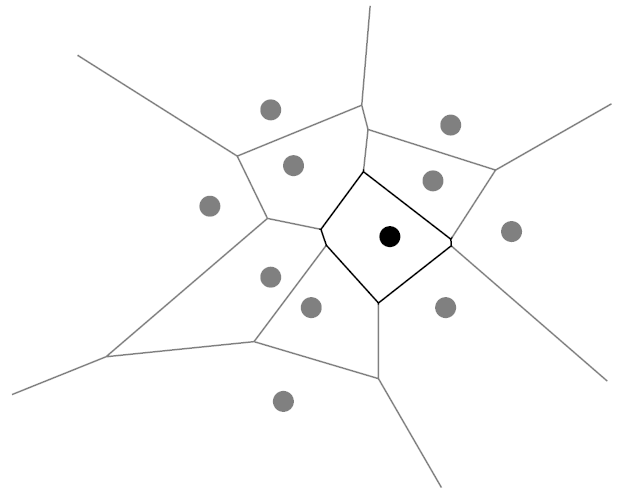
\includegraphics[width=0.32\textwidth]{FIGS/cell.png}
    \label{fig:cell}
  }\hspace{-3mm}
   \subfigure[]{
    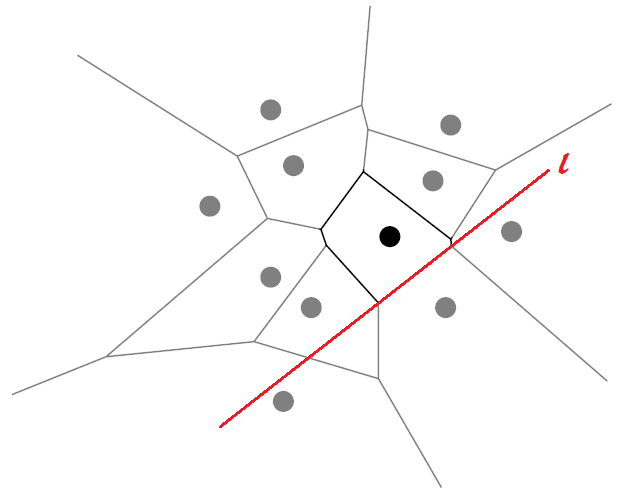
\includegraphics[width=0.32\textwidth]{FIGS/clippingLine.png}
    \label{fig:clippingline}
  }\\
  \subfigure[]{
    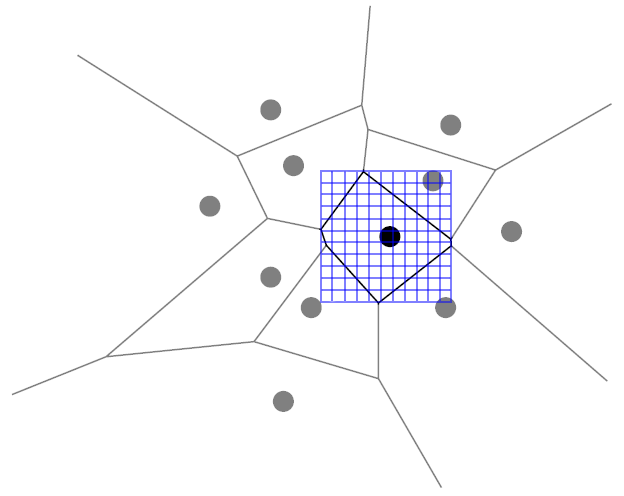
\includegraphics[width=0.32\textwidth]{FIGS/subpixel.png}
    \label{fig:subpixel}
  }\hspace{-3mm}
  \subfigure[]{
    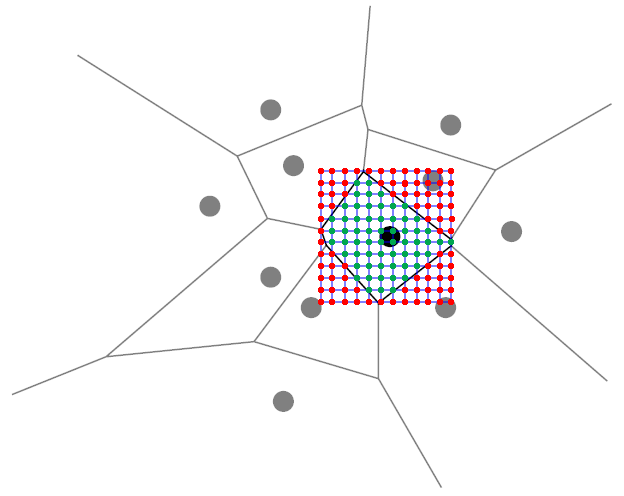
\includegraphics[width=0.32\textwidth]{FIGS/inandout.png}
    \label{fig:inOutTest}
  }\hspace{-3mm}
  \subfigure[]{
    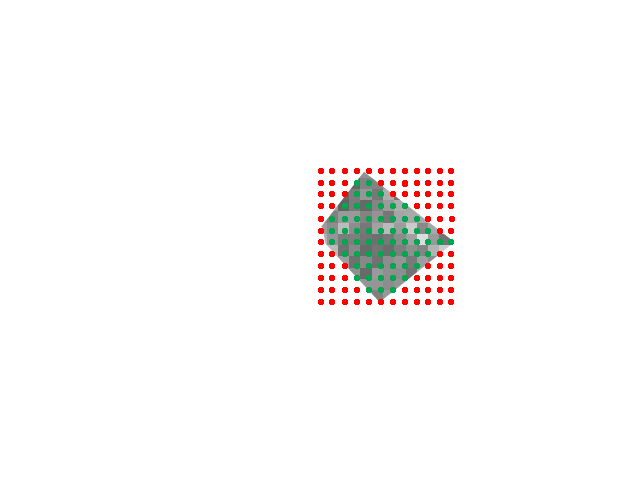
\includegraphics[width=0.32\textwidth]{FIGS/integral.png}
    \label{fig:integral}
  }\hspace{-3mm}
    \caption{The progress of computing voronoi diagram and redistributing stipples. \label{fig:createVoronoi}}
\end{figure*}
Next, voronoi method computes the voronoi region of given sample points(Fig. \ref{fig:voronoi}) using plane-sweep algorithm. 
After creating voronoi diagram of given points, the algorithm computes the centroid of a cell iteratively looping through all these points.
For example, with a given cell in Fig. \ref{fig:cell}, voronoi method calculates the line which is the extension of voronoi edge and is called clipping line(Fig. \ref{fig:clippingline}).
When two end points of voronoi edge are $\mathbf{x_1}=(x_1,y_1)$ and $\mathbf{x_2}=(x_2,y_2)$, the equation of clipping line is
\begin{equation}\label{eq:clippingLine}
\begin{gathered}
(y-y_1) = \frac{(y_2-y_1)}{(x_2-x_1)}(x-x_1)\\
(y-y_1)(x_2-x_1) = (y_2-y_1)(x-x_1)\\
(y_2-y_1)(x-x_1)-(y-y_1)(x_2-x_1)= 0\\
(y_2-y_1)x-(x_2-x_1)y+y_1(x_2-x_1)-x_1(y_2-y_1)=0\\
-(y_1-y_2)x+(x_1-x_2)y+x_1(y_1-y_2)-y_1(x_1-x_2)=0\\\\
\therefore ax+by+c=0 \\where\:a=-(y_1-y_2),\:b=(x_1-x_2),\:and\:c=x_1(y_1-y_2)-y_1(x_1-x_2).
\end{gathered}
\end{equation}
In the same way, we can generate clipping lines for all voronoi edges in a cell.\\\\
To obtain the integration of density $\rho(\mathbf{x})$, voronoi method creates regular grid on a cell with the user-specified number of subpixels(Fig. \ref{fig:subpixel}).
Using the clipping lines(Eq. \ref{eq:clippingLine}), we can test if a grid point is inside or outside of cell. If a grid point $\mathbf{x_g}=(x_g, y_g)$ satisfies $ax_g+by_g+c<0$ for all the clipping lines, it locates inside of a cell. The result of test is shown in Fig. \ref{fig:inOutTest}. The red points mean outside and the green points mean inside.
\\When grid points are inside, the algorithm obtains $\int_{A}\rho(\mathbf{x})dA$ and $\int_{A}\mathbf{x}\rho(\mathbf{x})dA$ with intensity $I(\mathbf{x_g})$ which has corresponding location to grid points in grayscale image(Fig. \ref{fig:integral}, Eq. \ref{eq:density}).
\begin{equation}\label{eq:density} .
\begin{gathered}
\int_{A}\rho(\mathbf{x})dA=\int I(\mathbf{x_g})\\
\int_{A}\mathbf{x}\rho(\mathbf{x})dA=\int \mathbf{x}I(\mathbf{x_g})=\int (x, y)I(\mathbf{x_g}).
\end{gathered}
\end{equation}
Substituting the results of Eq. \ref{eq:density} to Eq. \ref{eq:centroid}, we can generate new centroid $\mathbf{C_i}=(x_c, y_c)$,
which satisfies that $x_c=\frac{\int x\cdot I(\mathbf{x_g})}{\int I(\mathbf{x_g})}$ and $y_c=\frac{\int y\cdot I(\mathbf{x_g})}{\int I(\mathbf{x_g})}$.
This new centroids will be fed as sites into creating voronoi diagram step. Voronoi method repeats creating voronoi diagram and computing the centroid repeatedly until the average of displacement between points $\mathbf{x_i}$ and centroids $\mathbf{C_i}$ is small enough.
%Creating disks 
Finally, while creating the disks, voronoi method calculates the area of voronoi cell and computes the radius fits to this area. 
%%%%%%%%%%%%%%%%%%%%%%%%%%%%%%%%%%%%%%%%%%%%%%%%%%%%%%%%%%%%%%%%%%%%%%%%%%%%%%%%%%%%%%%%%%%%%%%%%%%%%%%%%%%%
\section{Example Outputs}\label{outputs}
Here are the simple results of both methods with given examples(Fig. \ref{fig:simple_results1} and Fig. \ref{fig:simple_results2}). As mentioned in the paper\cite{secord02}, the results of hedcuter method has some voids and overlapping stipples with same conditions. This is because of different densities at each stipple levels. \\
I also compare the output of two methods with various conditions in the following subsections. 
%%%%%%%%%%%%%%%%%%%%%%%%%%%%%%%%%%%%%%%%%%%%%%%%%%%%%%%%%%%%%%%%%%%%%%%%%%%%%%%%%%%%%%%%%%%%%%%%%%%%%%%%%%%%
\subsection{same condition with multiple excution}
Even if the initial condition is same, the result shows that hedcuter method generates different results at each time. With the same input image and the same number of initial samples, the points composed of squirrel head has different distribution in hedcuter method(the red squares in the first row images of Fig. \ref{fig:sameInput}). However, the results of voronoi method are exactly same(the second row images of Fig. \ref{fig:sameInput}). This is because two methods use different technique to generate samples. The hedcuter method uses random function with time seed(rand(time(NULL)), which produces different distributions when it calls. In case of voronoi method, it uses Mersenne twister(
boost::mt19937) and it generates the same sample points with the same seed. Different initial points lead to different output in hedcuter method.
\begin{figure*}[hbt]
 \centering
 \subfigure[]{
    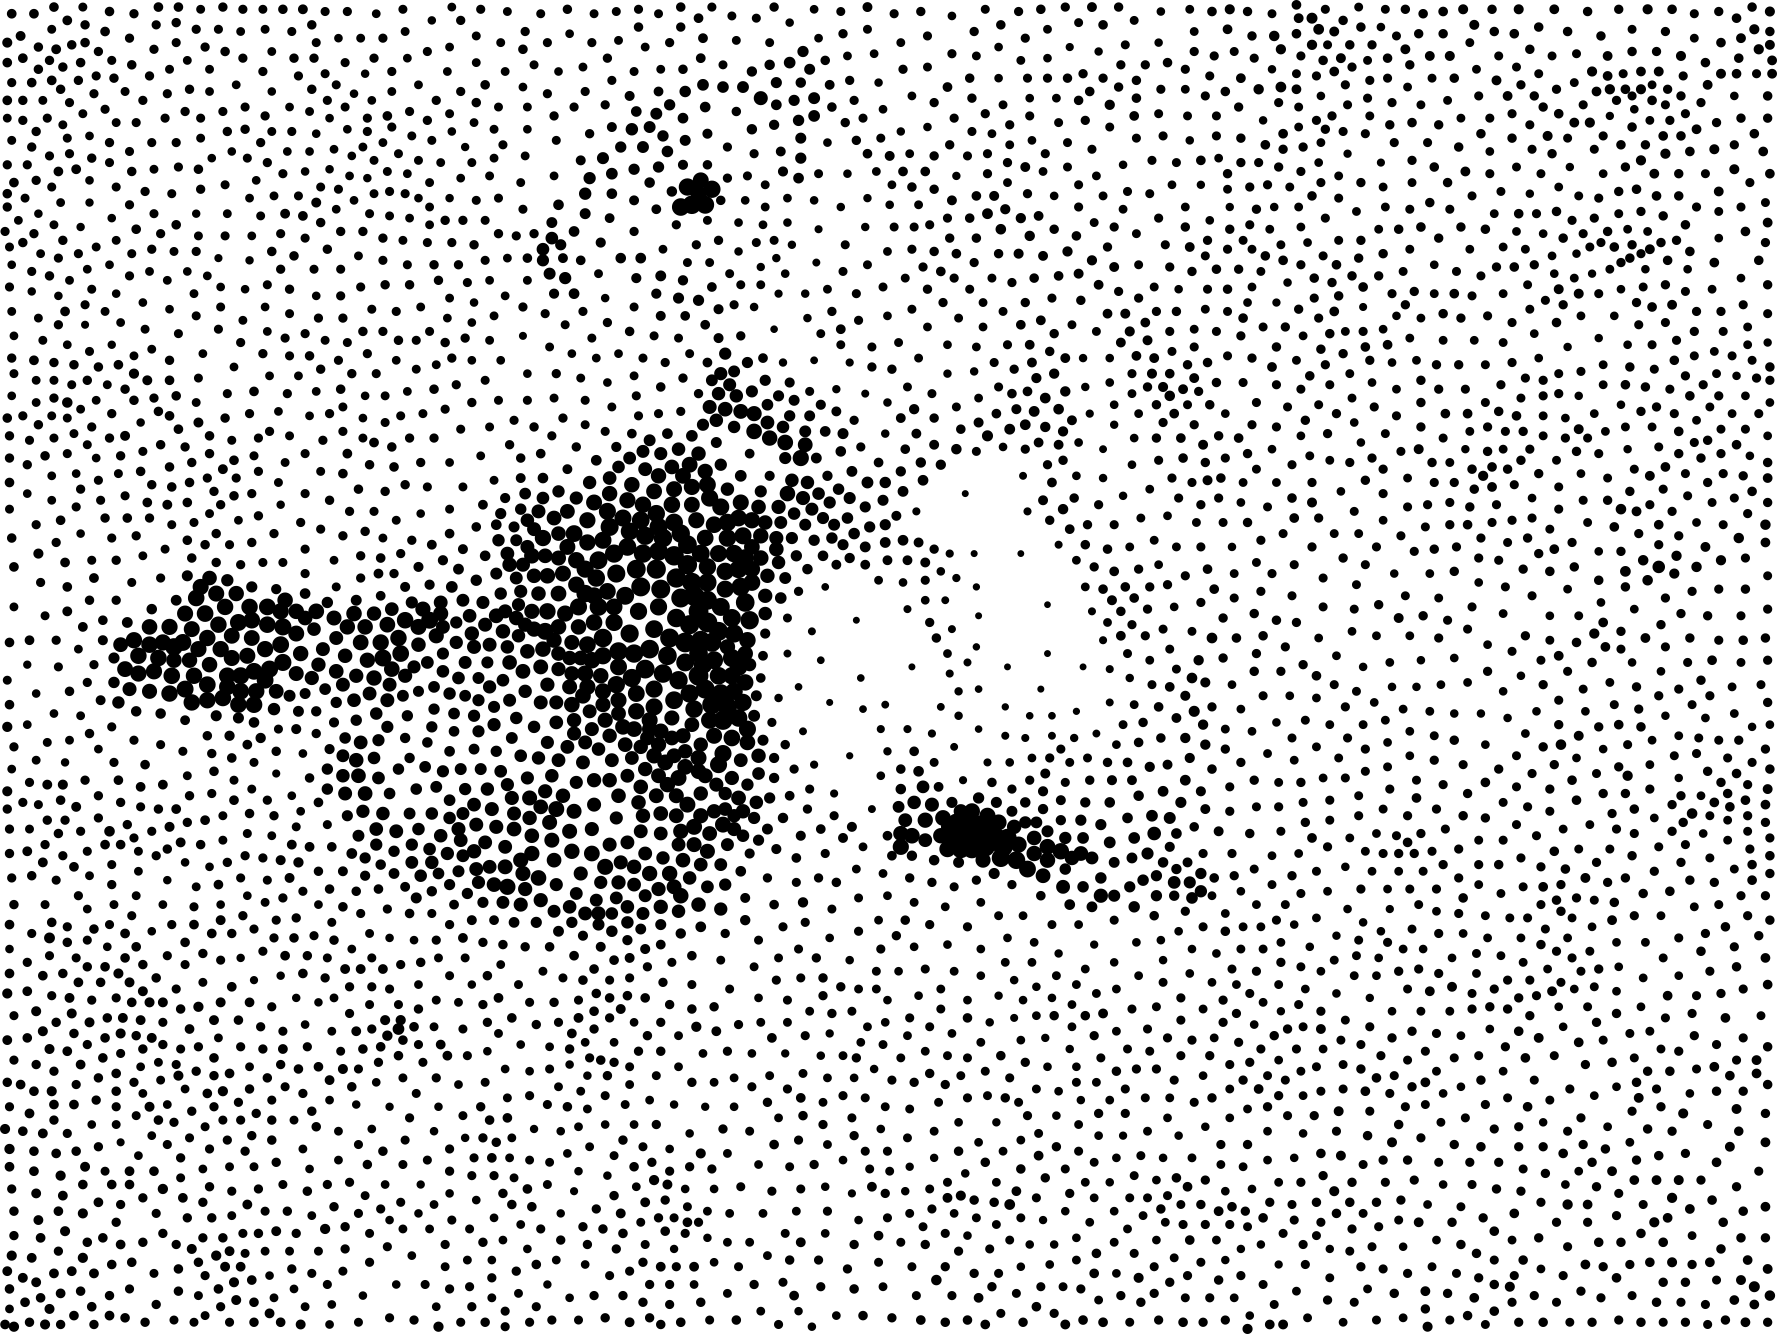
\includegraphics[width=0.32\textwidth]{FIGS/sameInput/squirrel-h-5000_01.png}
    \label{fig:sameInput1}
  }\hspace{-3mm}
  \subfigure[]{
    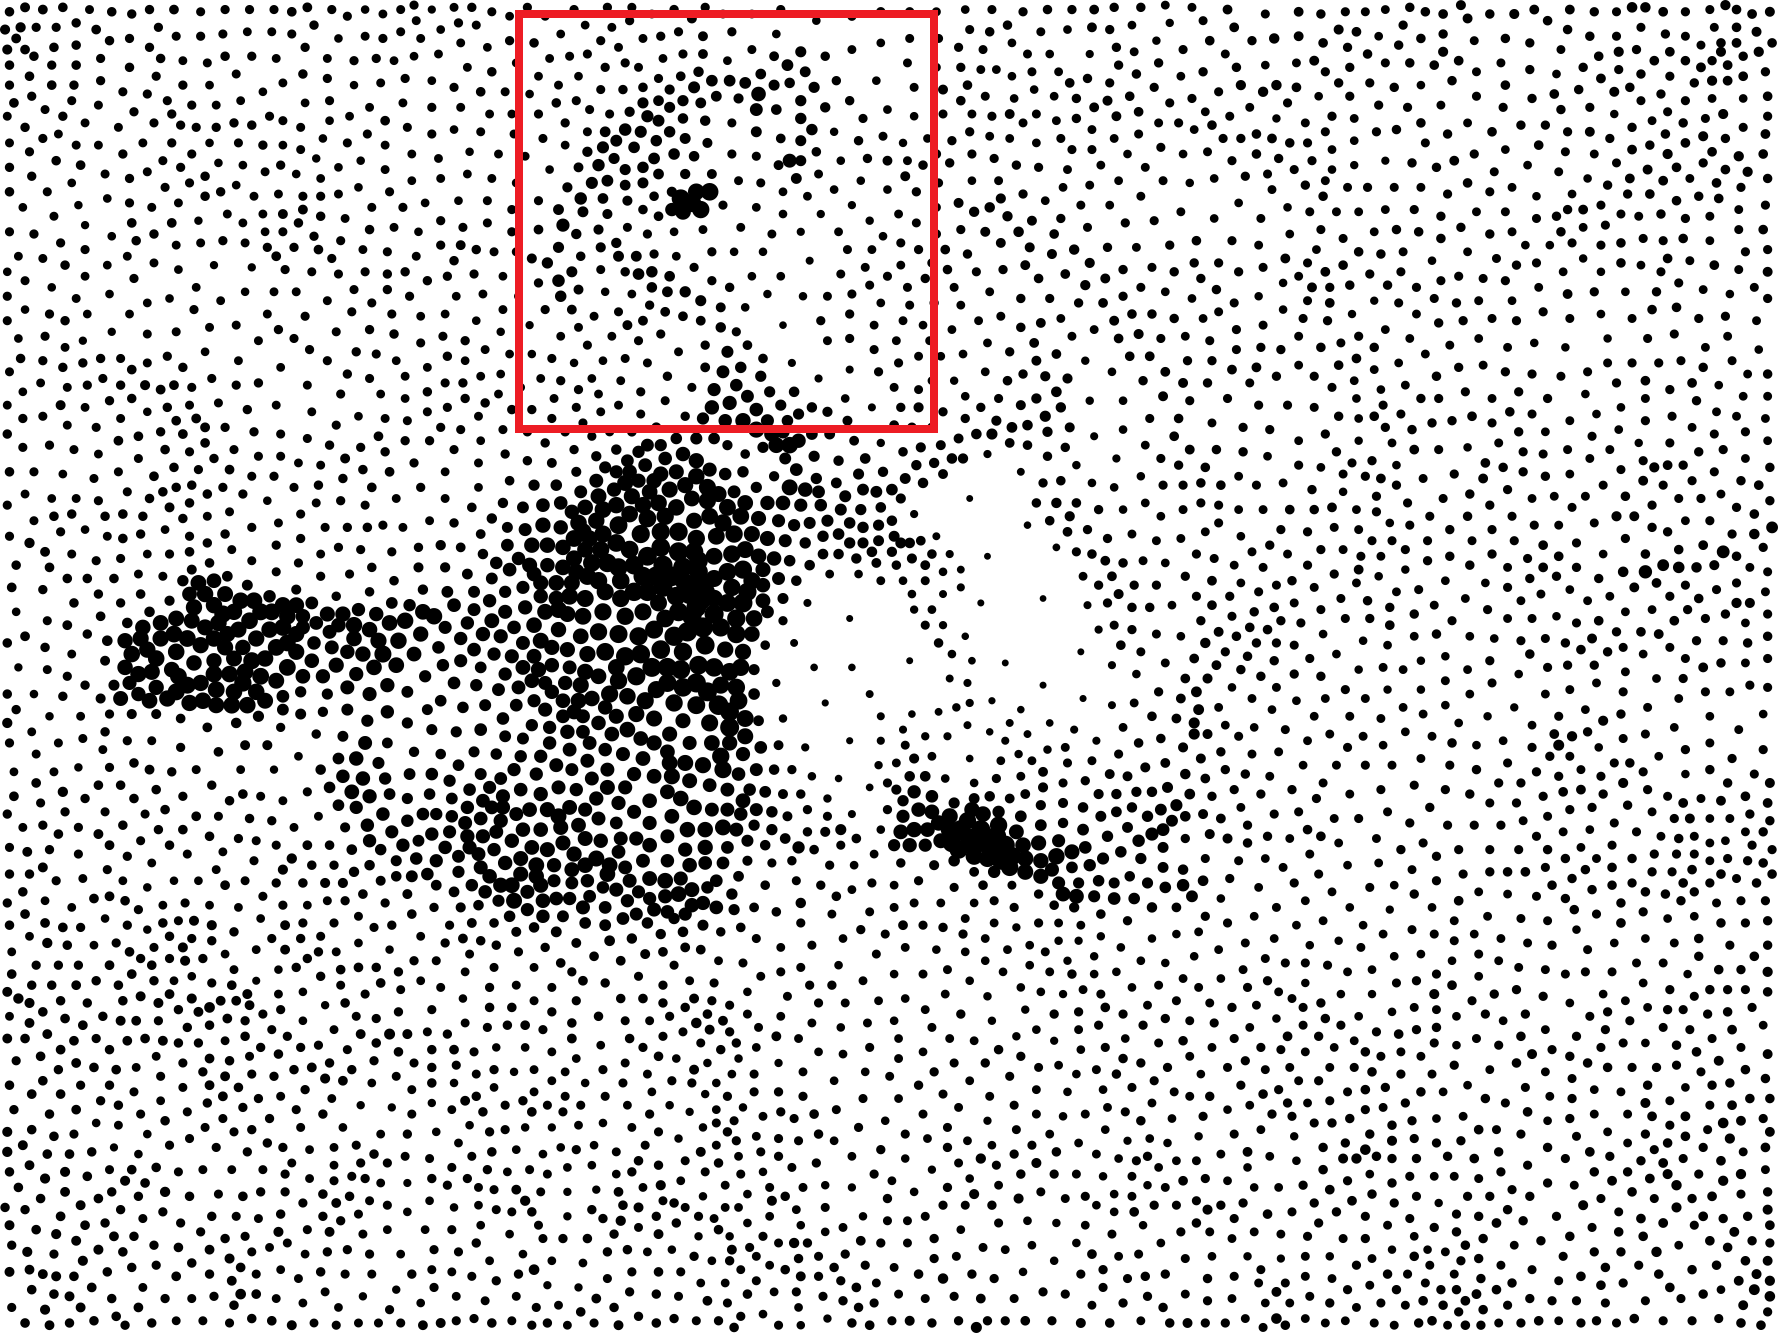
\includegraphics[width=0.32\textwidth]{FIGS/sameInput/squirrel-h-5000_02.png}
    \label{fig:sameInput2}
  }\hspace{-3mm}
  \subfigure[]{
    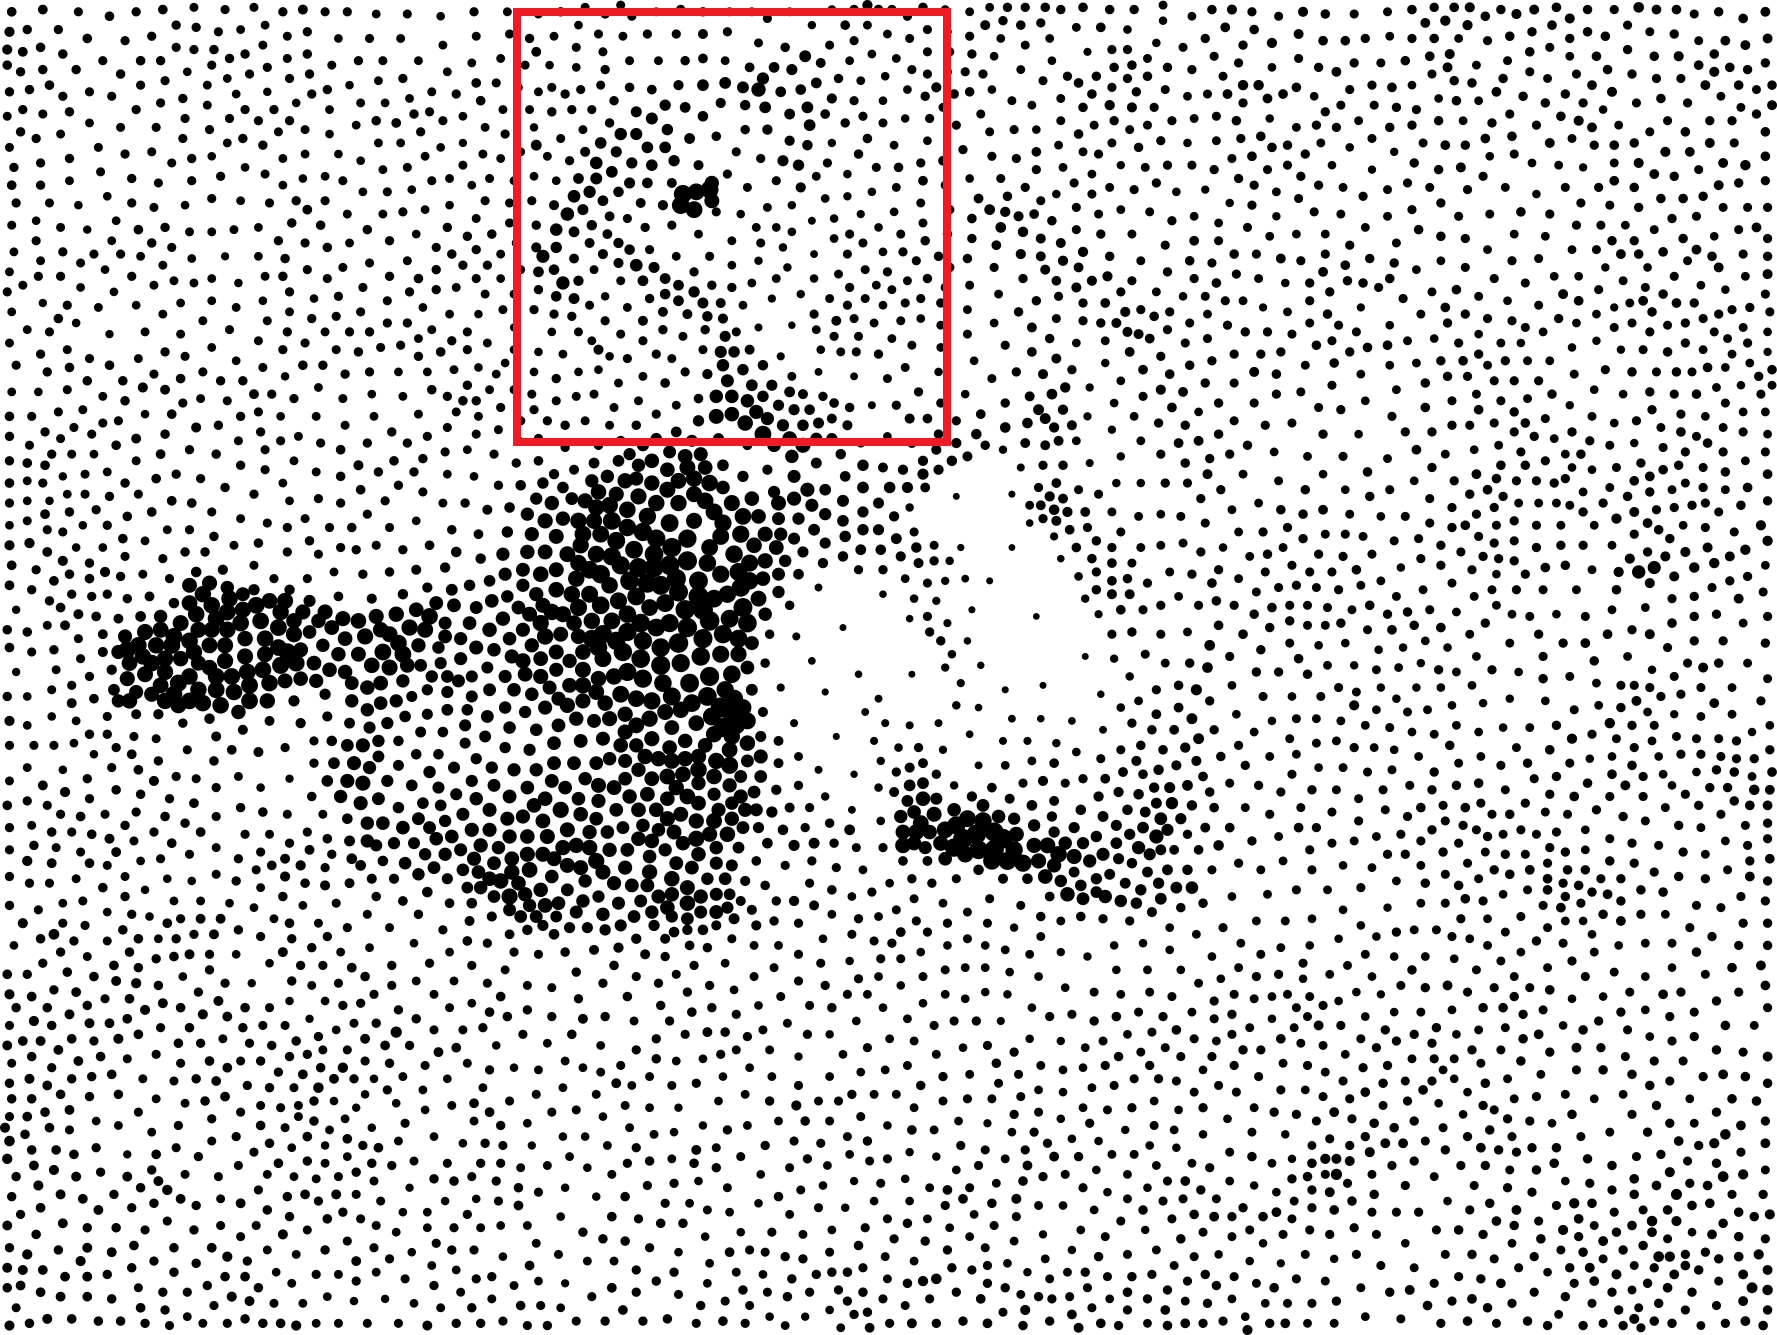
\includegraphics[width=0.32\textwidth]{FIGS/sameInput/squirrel-h-5000_03.png}
    \label{fig:sameInput3}
  }\\
  \subfigure[]{
    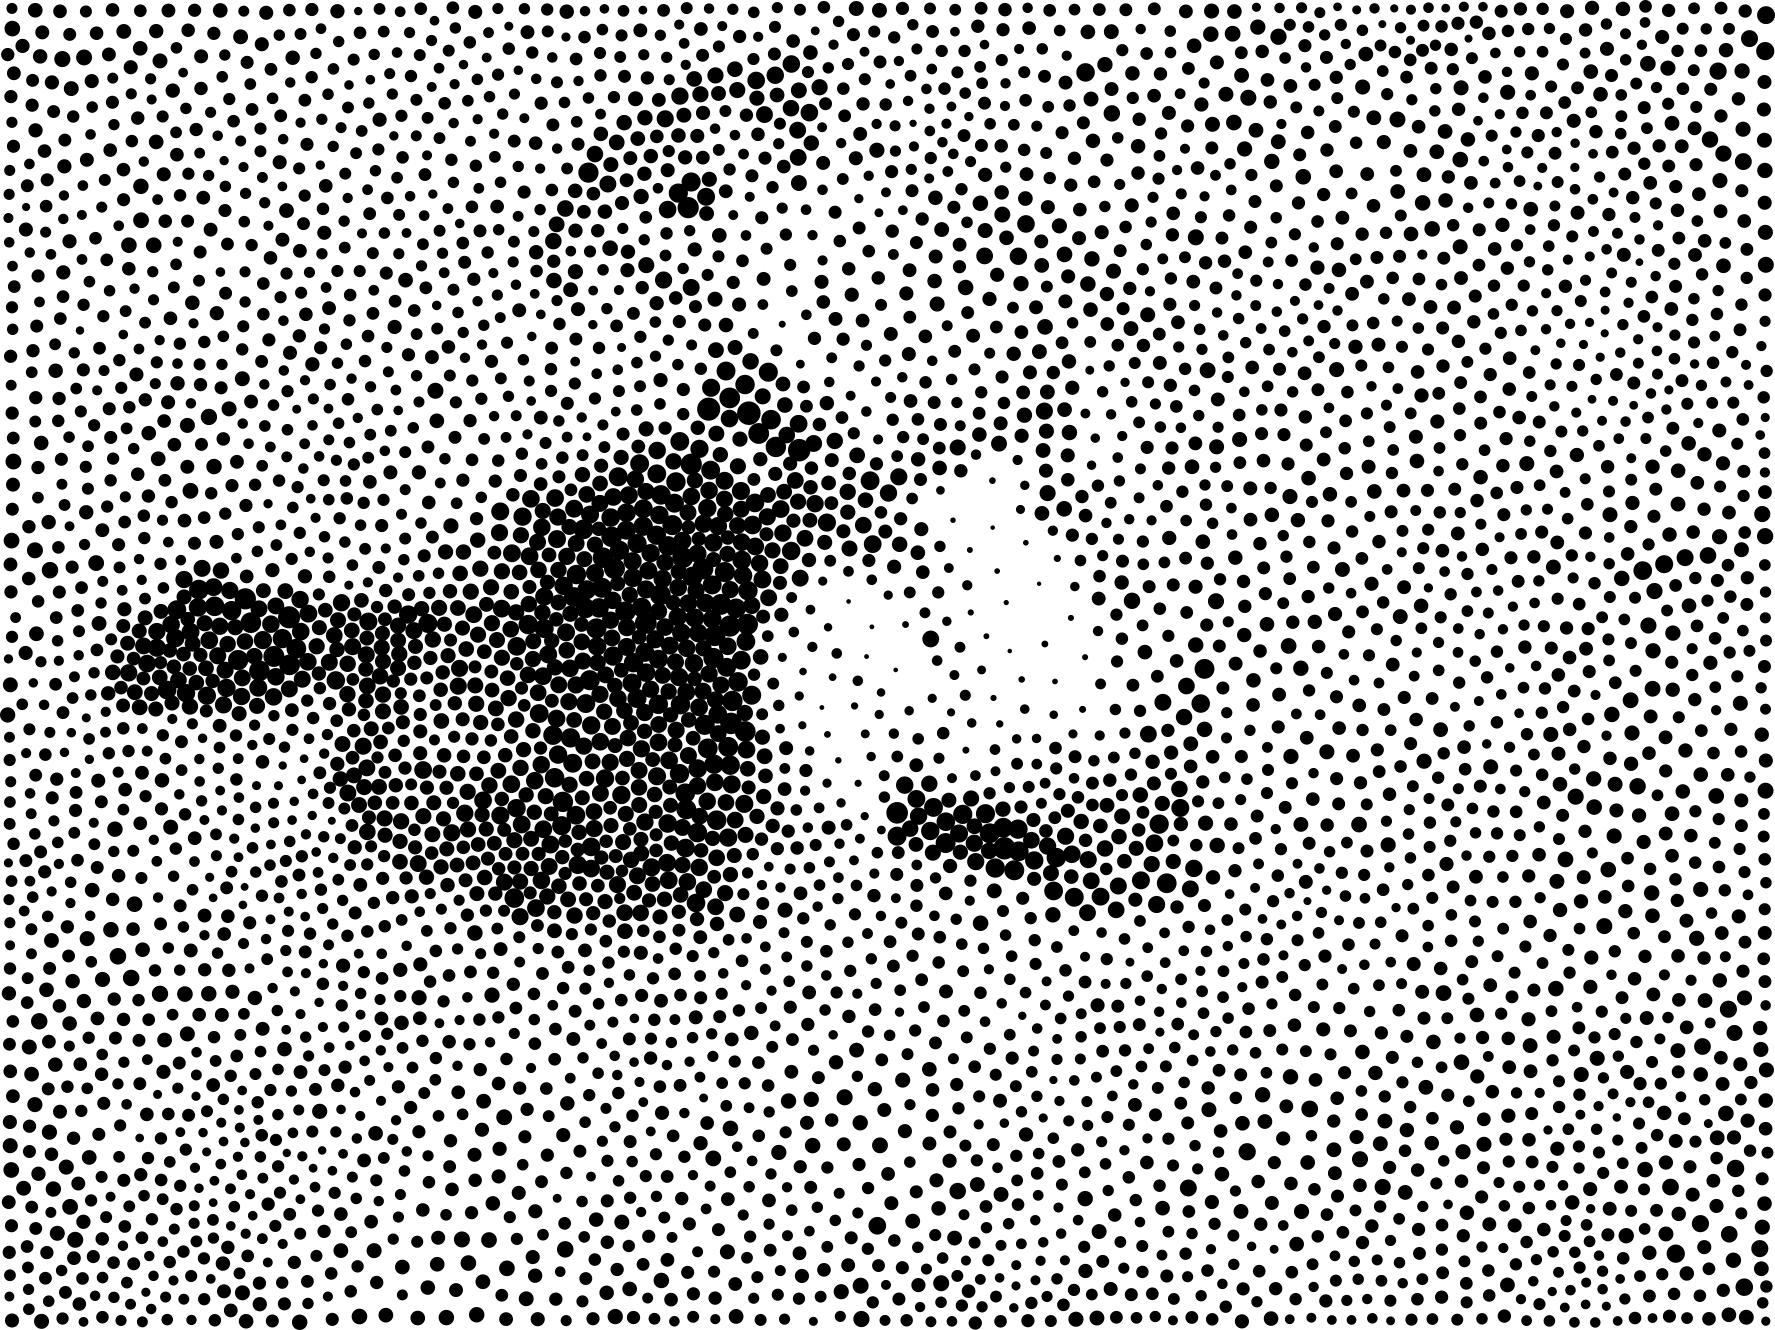
\includegraphics[width=0.32\textwidth]{FIGS/sameInput/squirrel-stippler_01.png}
    \label{fig:sameInput4}
  }\hspace{-3mm}
  \subfigure[]{
    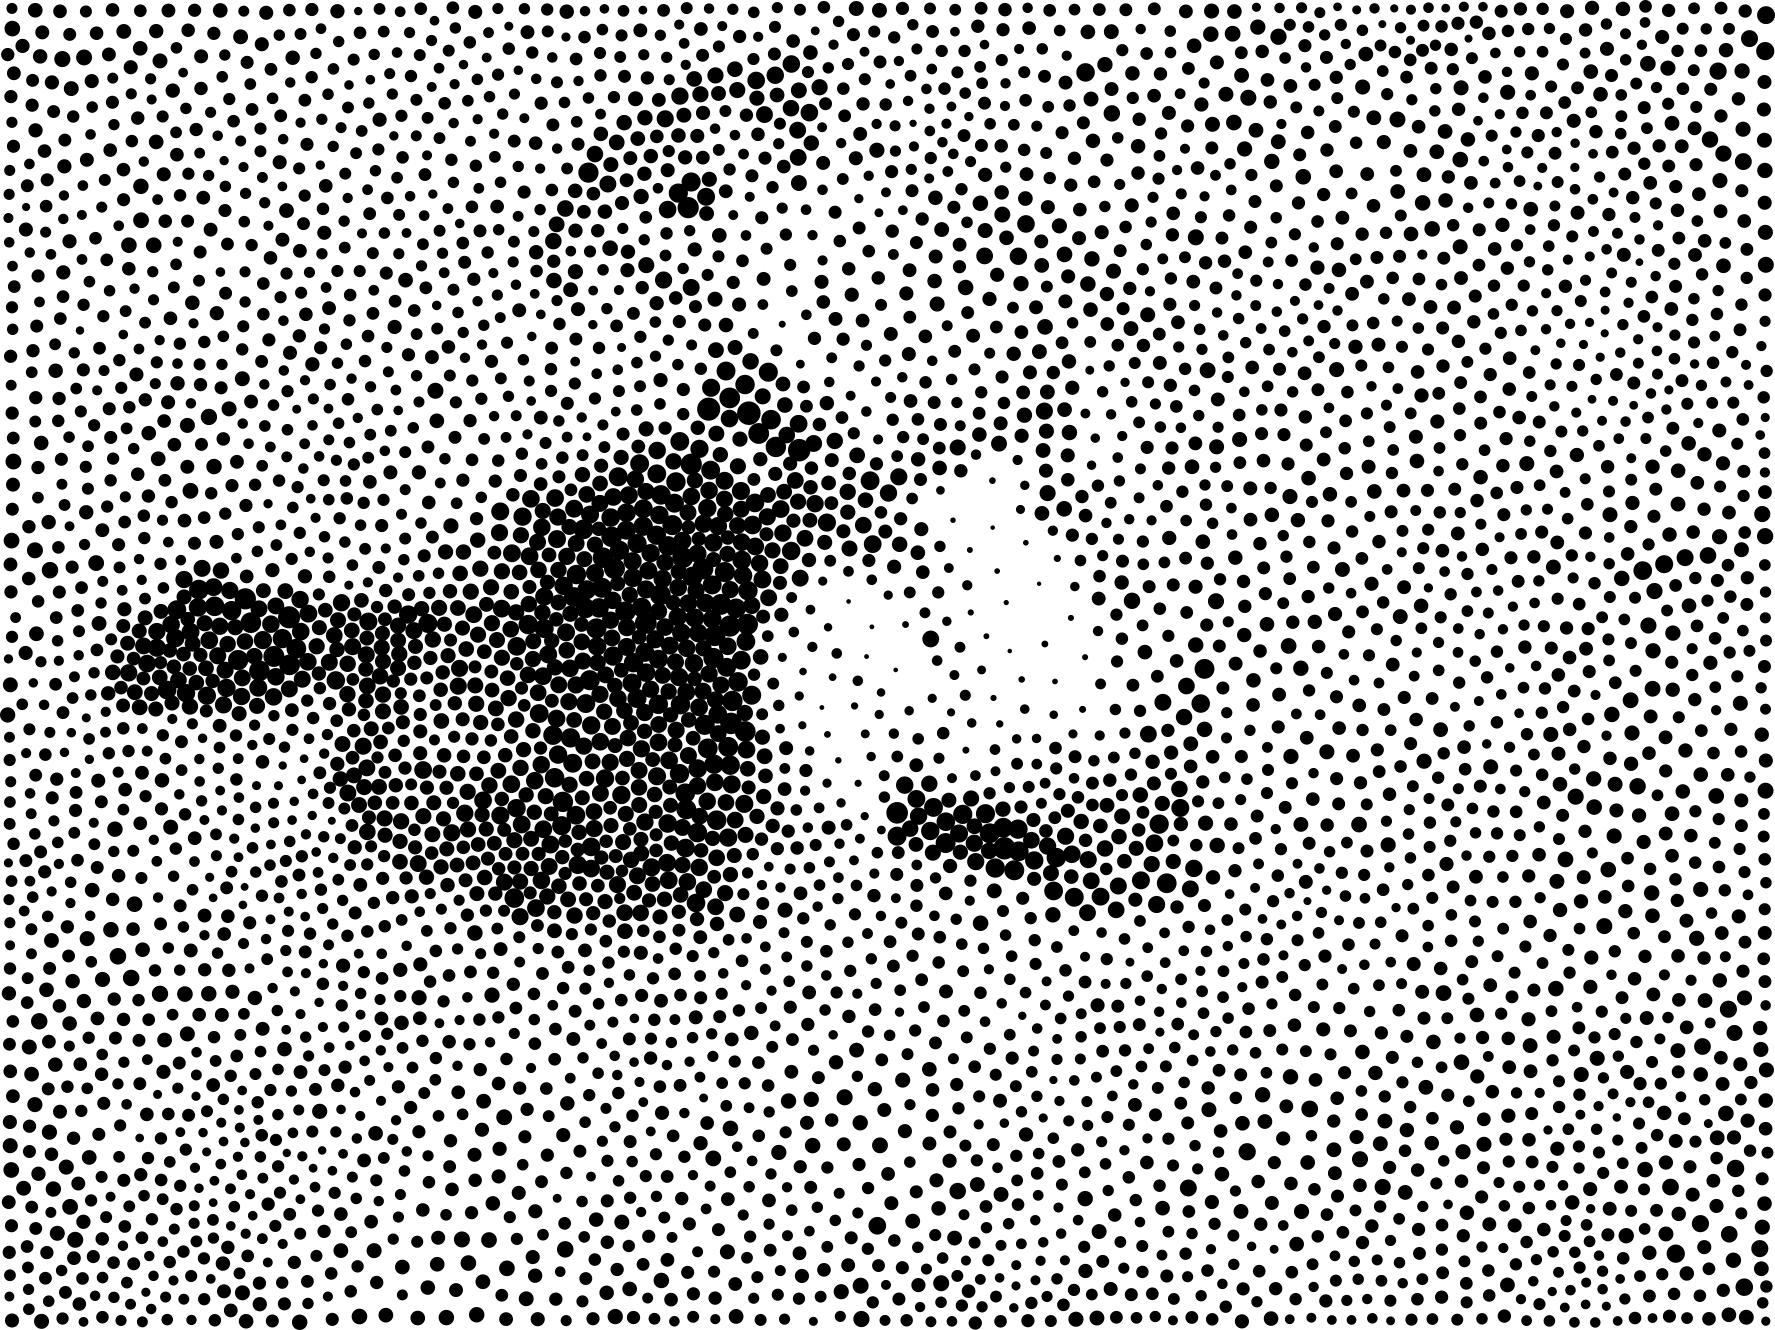
\includegraphics[width=0.32\textwidth]{FIGS/sameInput/squirrel-stippler_02.png}
    \label{fig:sameInput5}
  }\hspace{-3mm}
  \subfigure[]{
    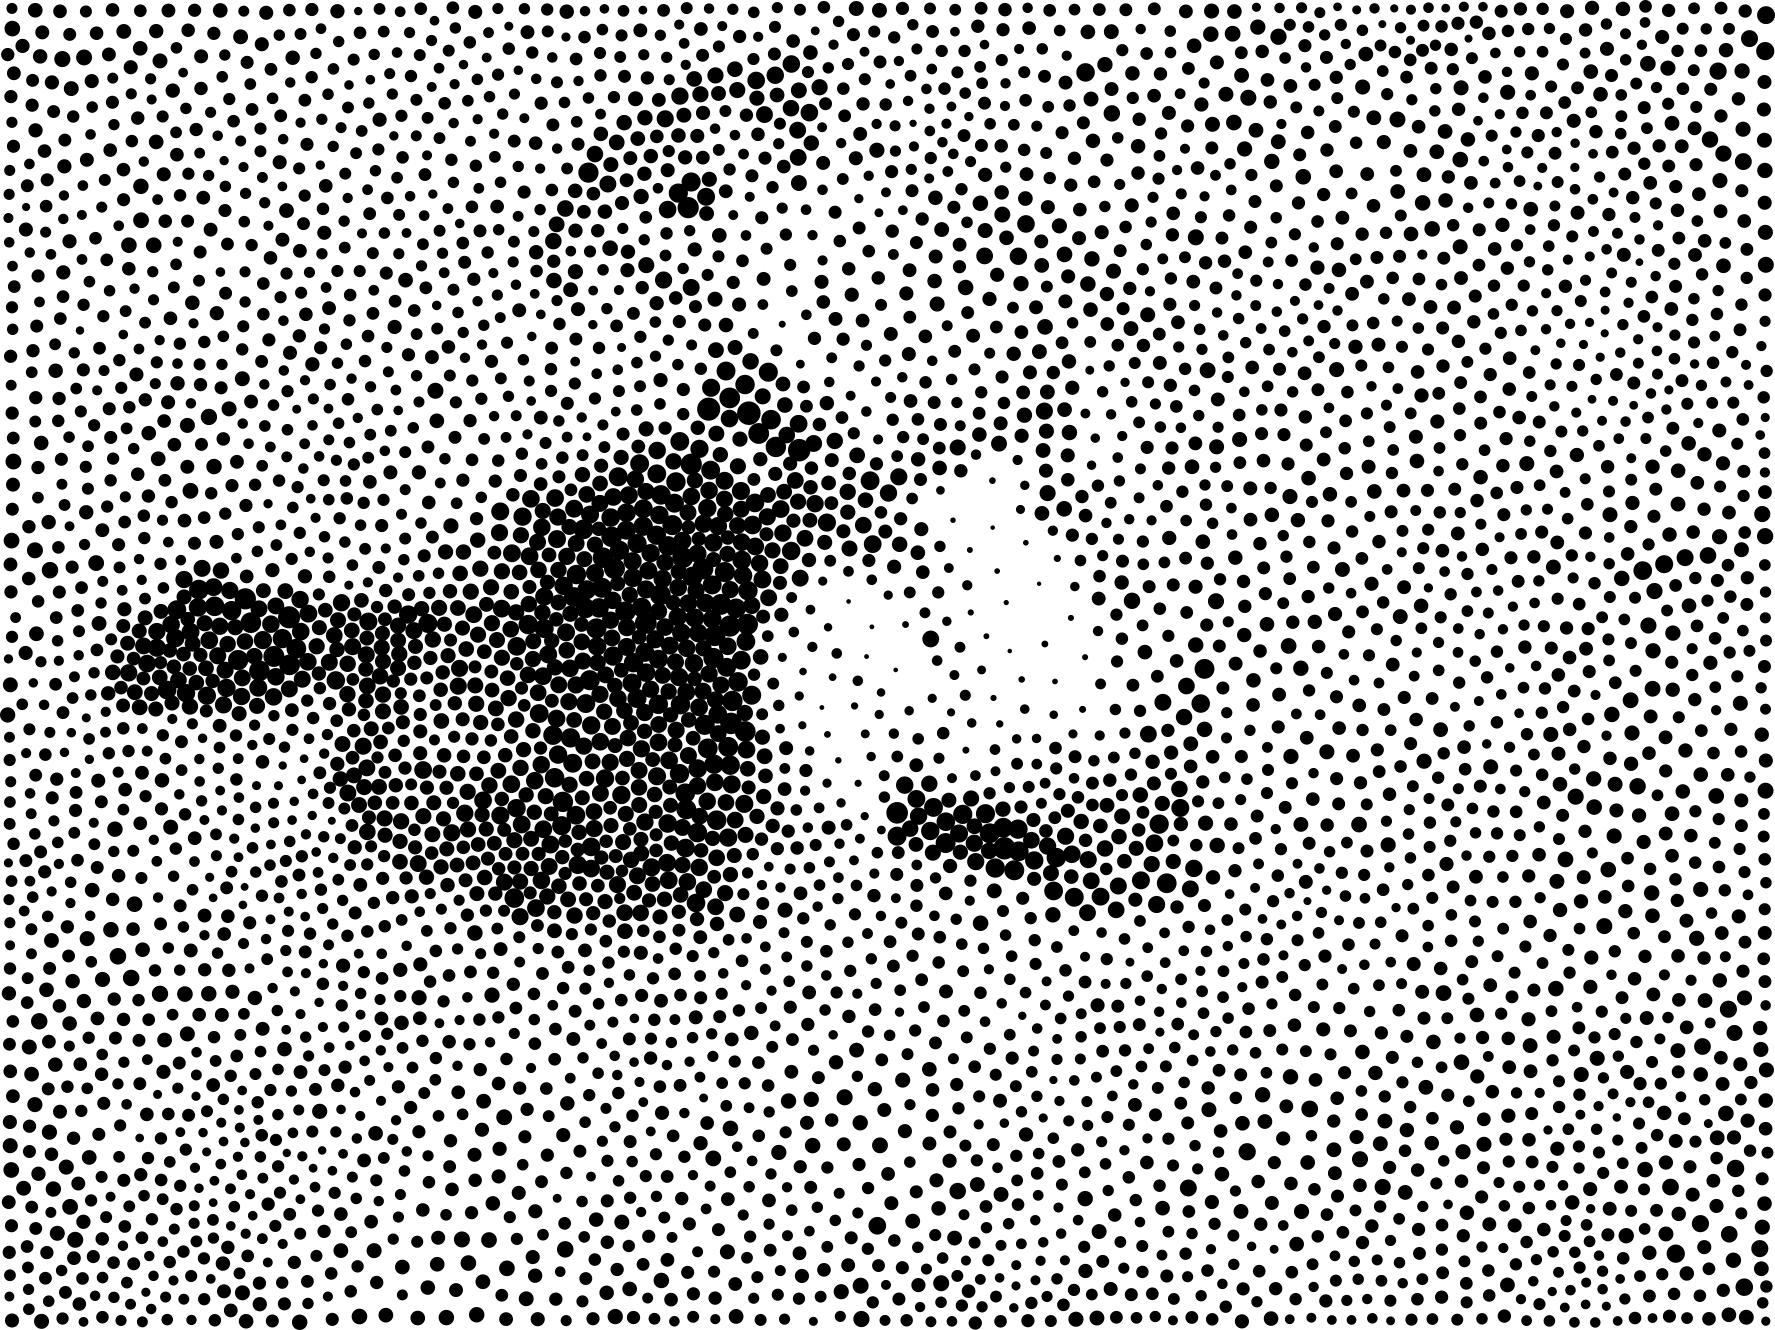
\includegraphics[width=0.32\textwidth]{FIGS/sameInput/squirrel-stippler_03.png}
    \label{fig:sameInput6}
  }
    \caption{The output result of same initial condition for both methods. The first row is the result of hedcuter method, and the second row is the result of voronoi method. \label{fig:sameInput}}
\end{figure*}
%%%%%%%%%%%%%%%%%%%%%%%%%%%%%%%%%%%%%%%%%%%%%%%%%%%%%%%%%%%%%%%%%%%%%%%%%%%%%%%%%%%%%%%%%%%%%%%%%%%%%%%%%%%%
\subsection{size of input image}
Various size of input image brings interesting result(Fig. \ref{fig:cat_size}). From the left to the right column, the size of each image is 500x333, 750x499, 1500x997 and 3000x1993 with the same number of sample points. In case of voronoi method, the size is not an significant factor to stippling quality. However, hedcuter method generates more good quality stippling when the size of input image goes bigger. For example, the patterns on cat's head and whiskers(marked by blue square)becomes distinct and clustering of sample points(marked by red square) tends to disappear. This is caused by the nature of discrete voronoi diagram, as mentioned in \cite{secord02}. If the resolution of image is lower, the relative error of the calculated centroid location is bigger. Voronoi method uses gaussian numerical integration to find the area with the density information and calculate the radius fits to this volume. This technique preserves the tone of stippling. 
\begin{figure*}[hbt]
   \subfigure[]{
    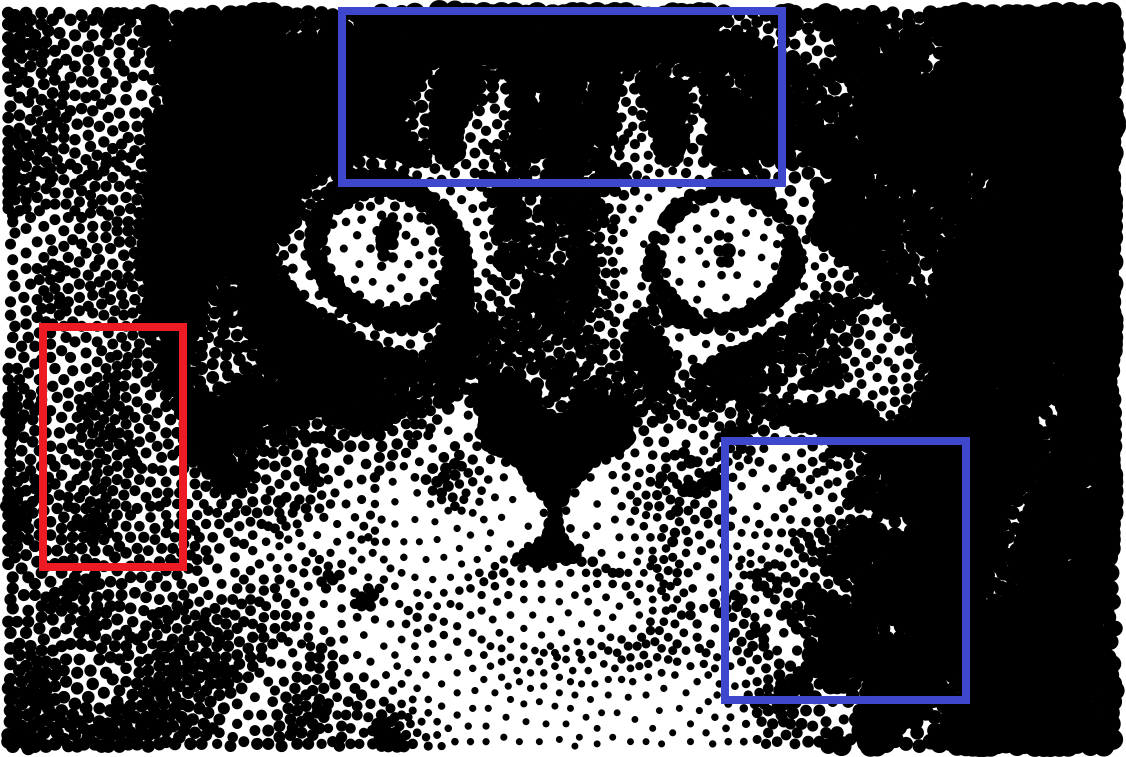
\includegraphics[width=0.22\textwidth]{FIGS/size/cat-xsmall-7500.png}
    \label{fig:cat_xs}
  }\hspace{-3mm}
  \subfigure[]{
    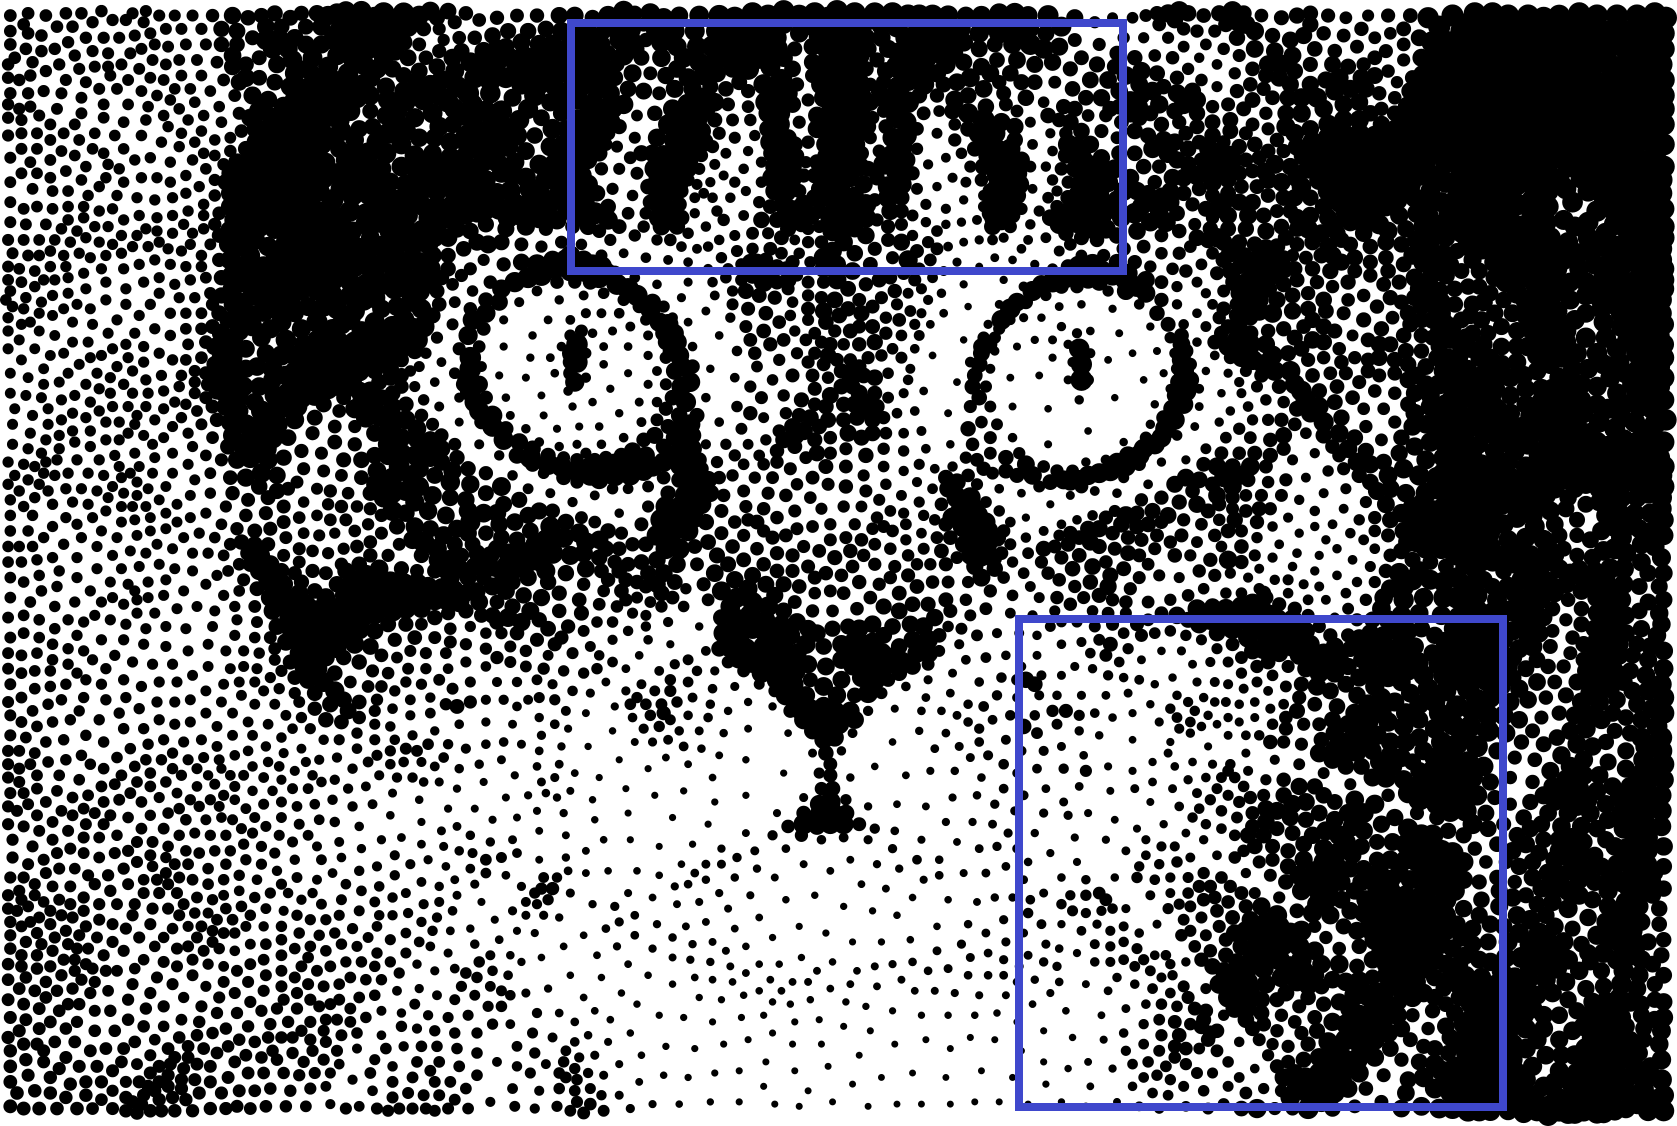
\includegraphics[width=0.22\textwidth]{FIGS/size/cat-small-7500.png}
    \label{fig:cat_s}
  }\hspace{-3mm}
  \subfigure[]{
    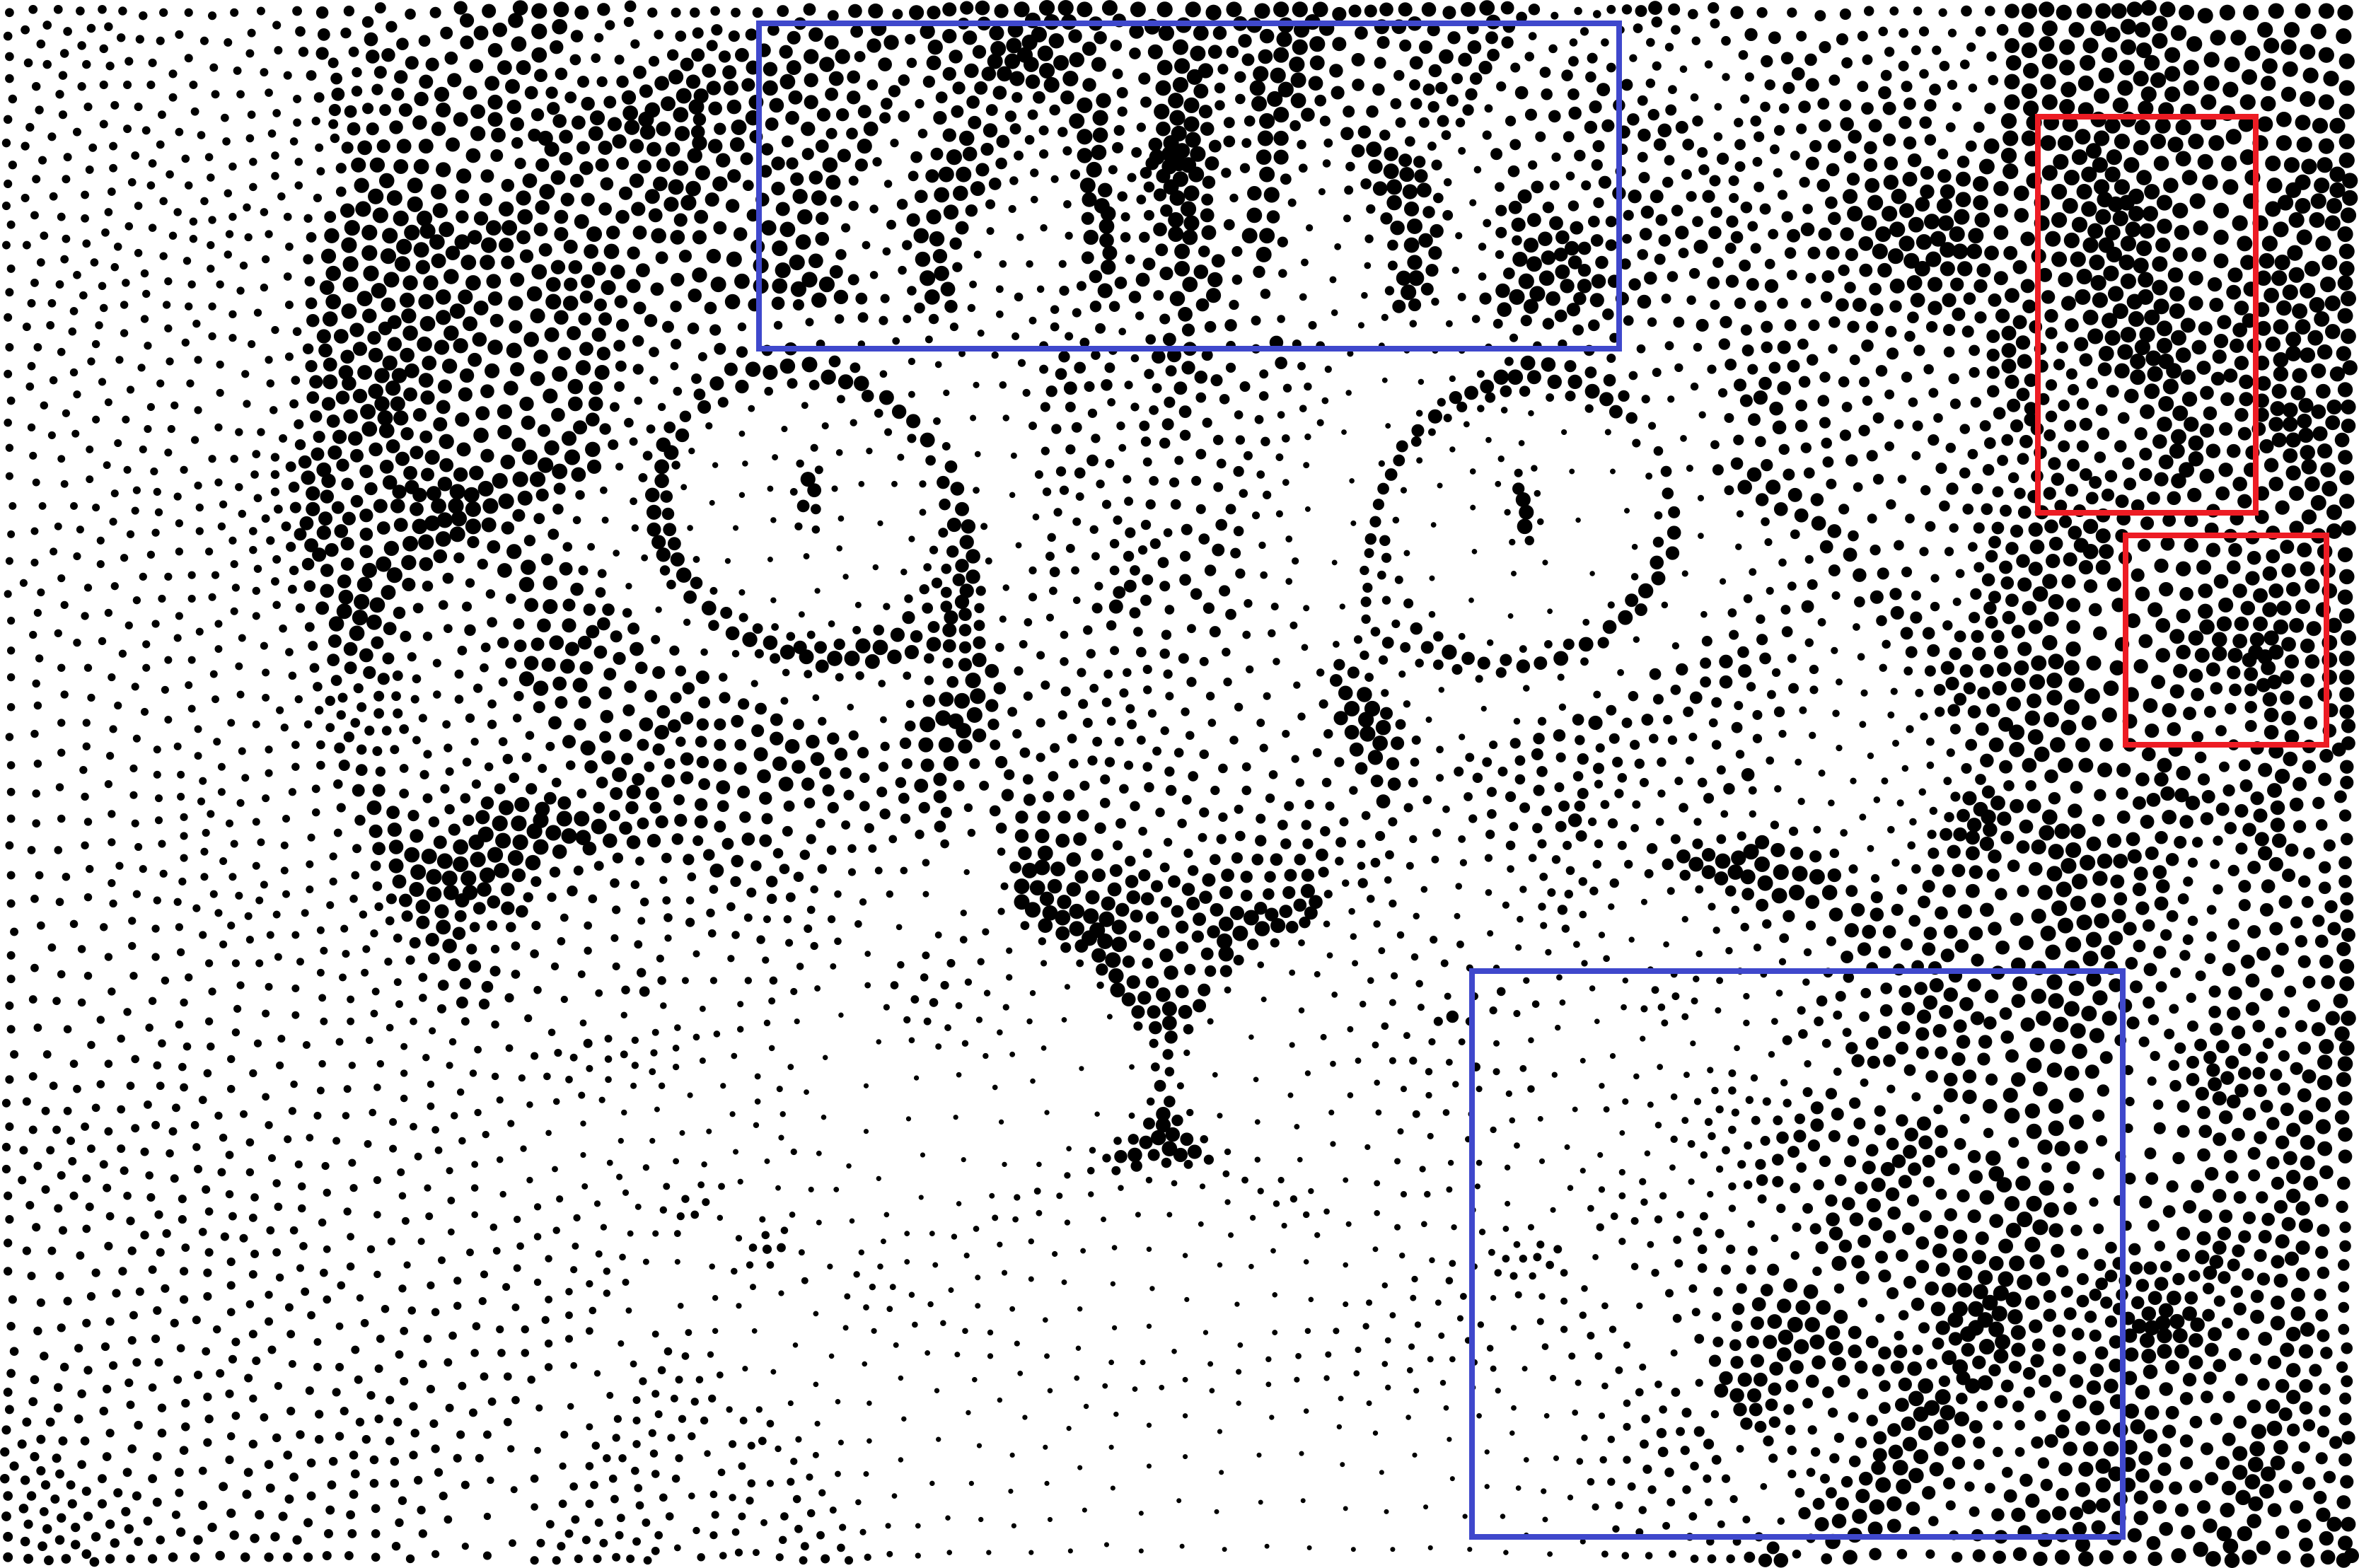
\includegraphics[width=0.22\textwidth]{FIGS/size/cat-middle-7500.png}
    \label{fig:cat_s}
  }\hspace{-3mm}
  \subfigure[]{
    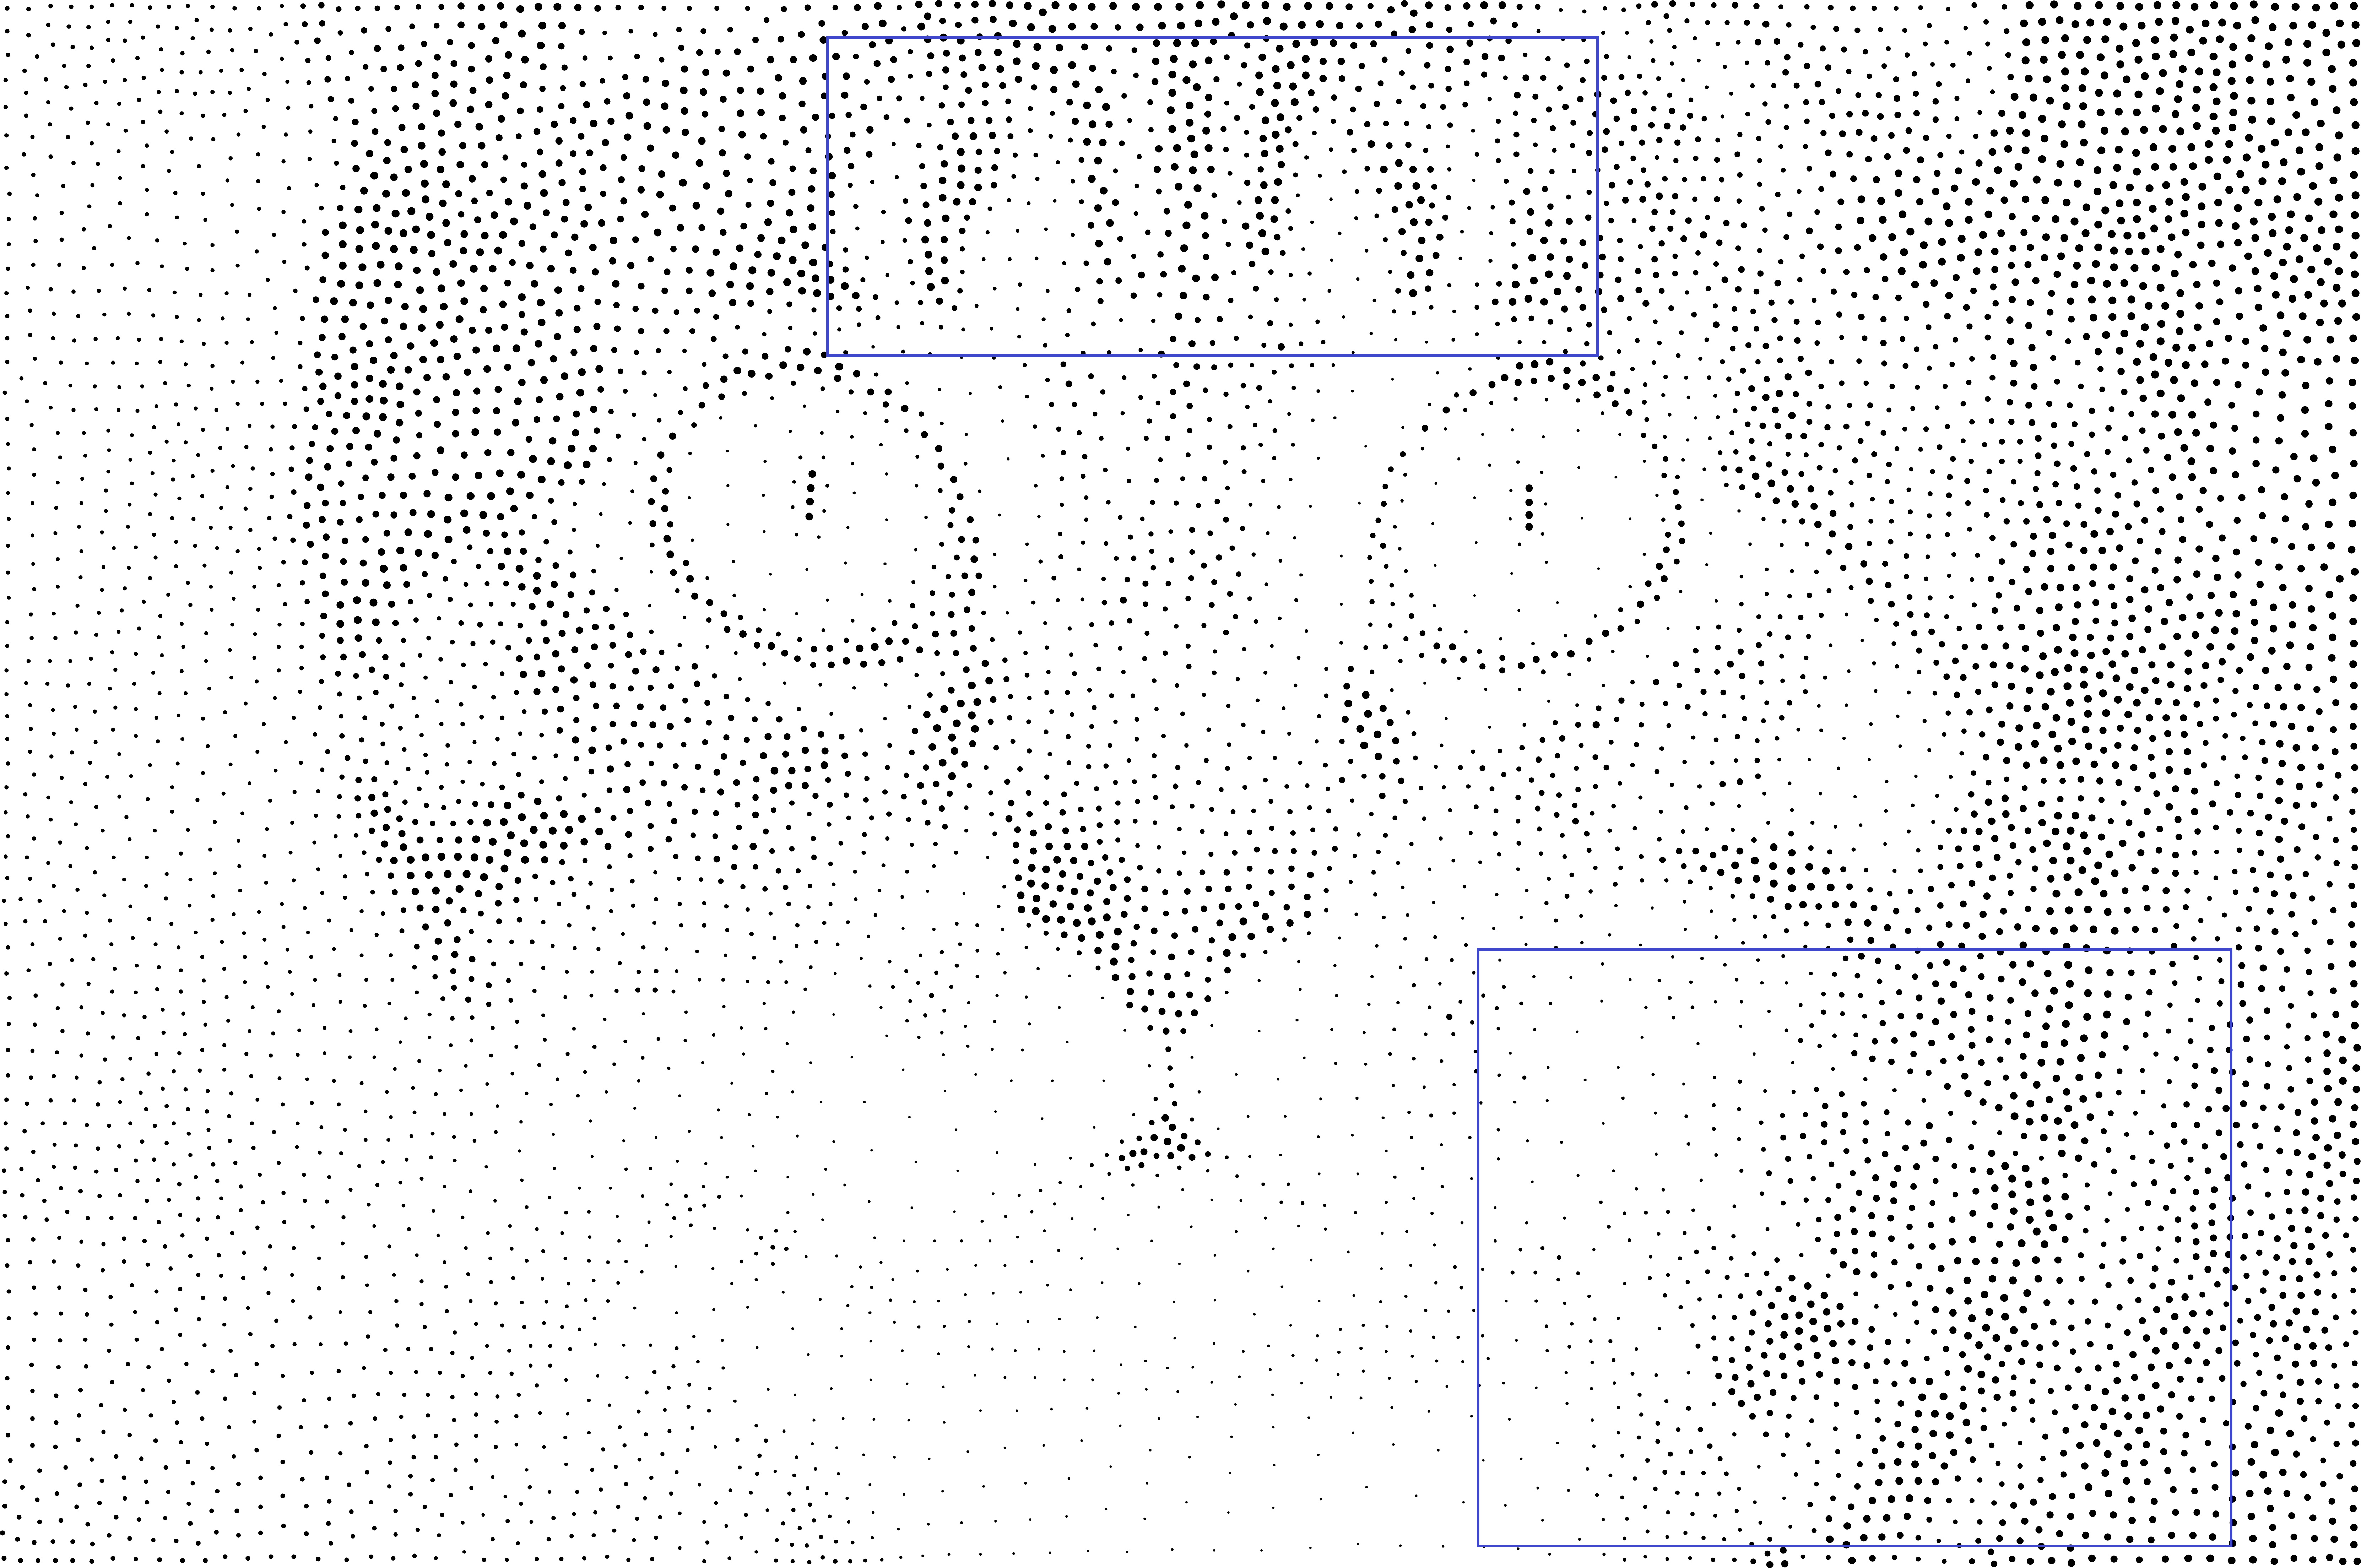
\includegraphics[width=0.22\textwidth]{FIGS/size/cat-large-7500.png}
    \label{fig:cat_s}
  }\\
  \subfigure[]{
    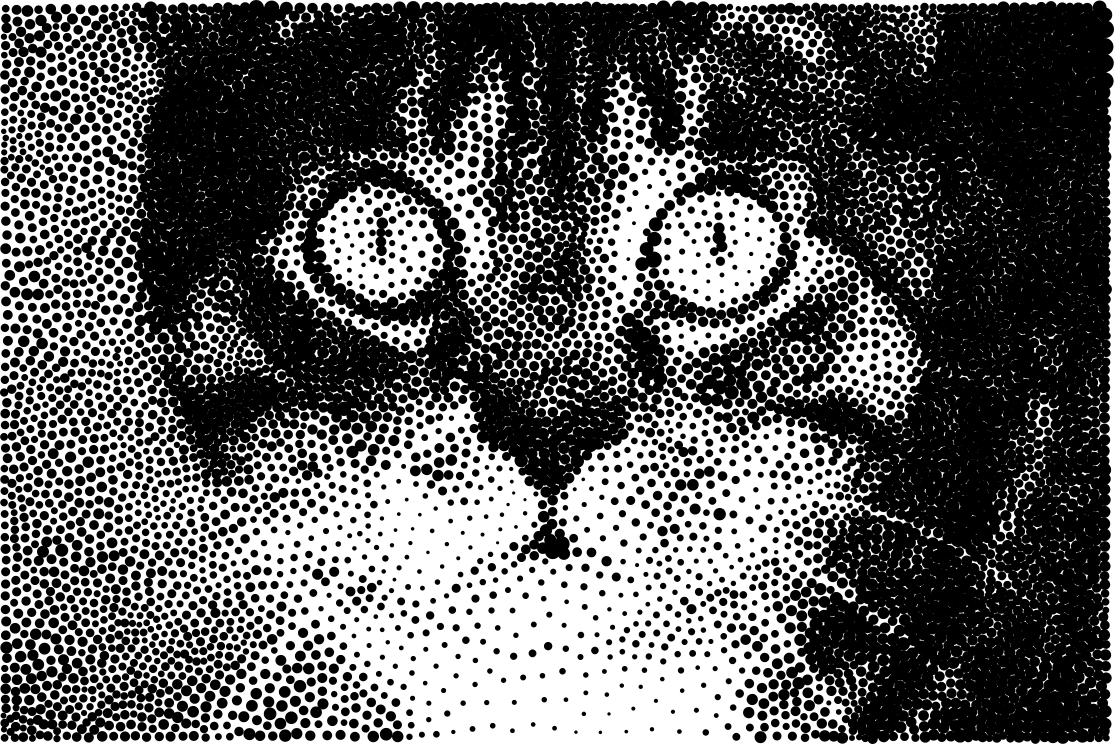
\includegraphics[width=0.22\textwidth]{FIGS/size/cat-xsmall-stippler.png}
    \label{fig:cat_xs}
  }\hspace{-3mm}
  \subfigure[]{
    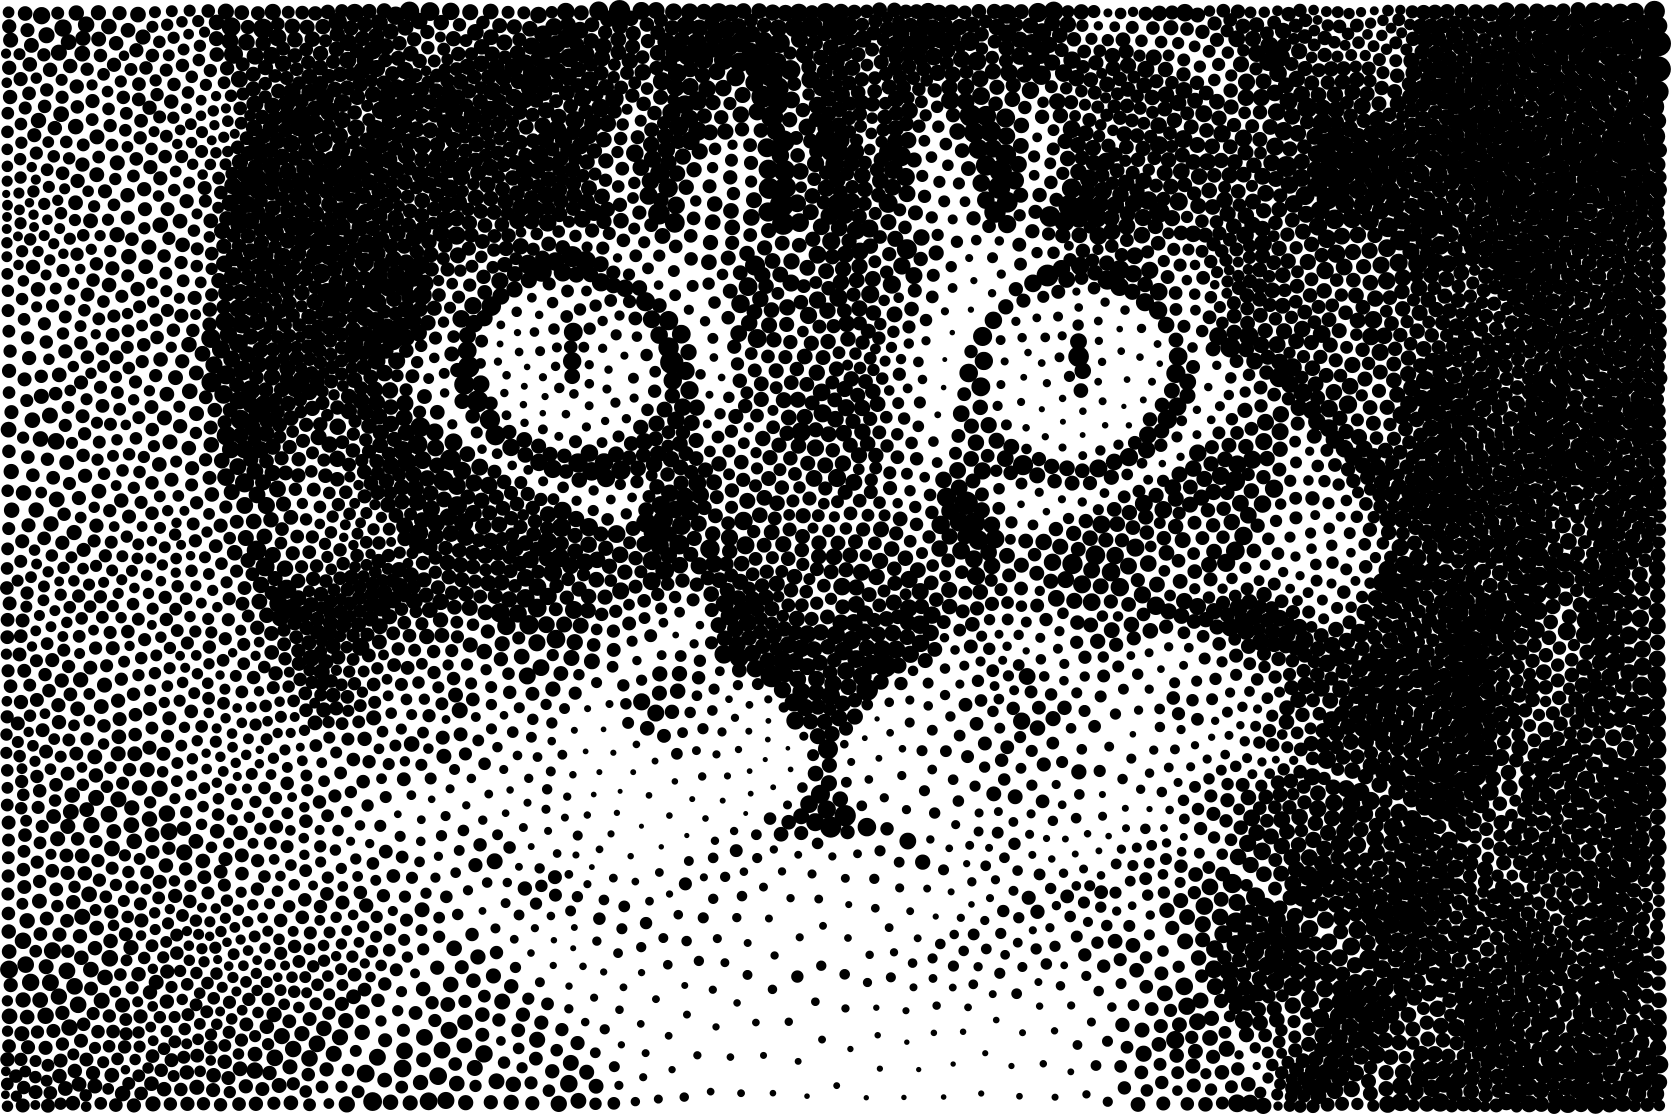
\includegraphics[width=0.22\textwidth]{FIGS/size/cat-small-stippler.png}
    \label{fig:cat_s}
  }\hspace{-3mm}
  \subfigure[]{
    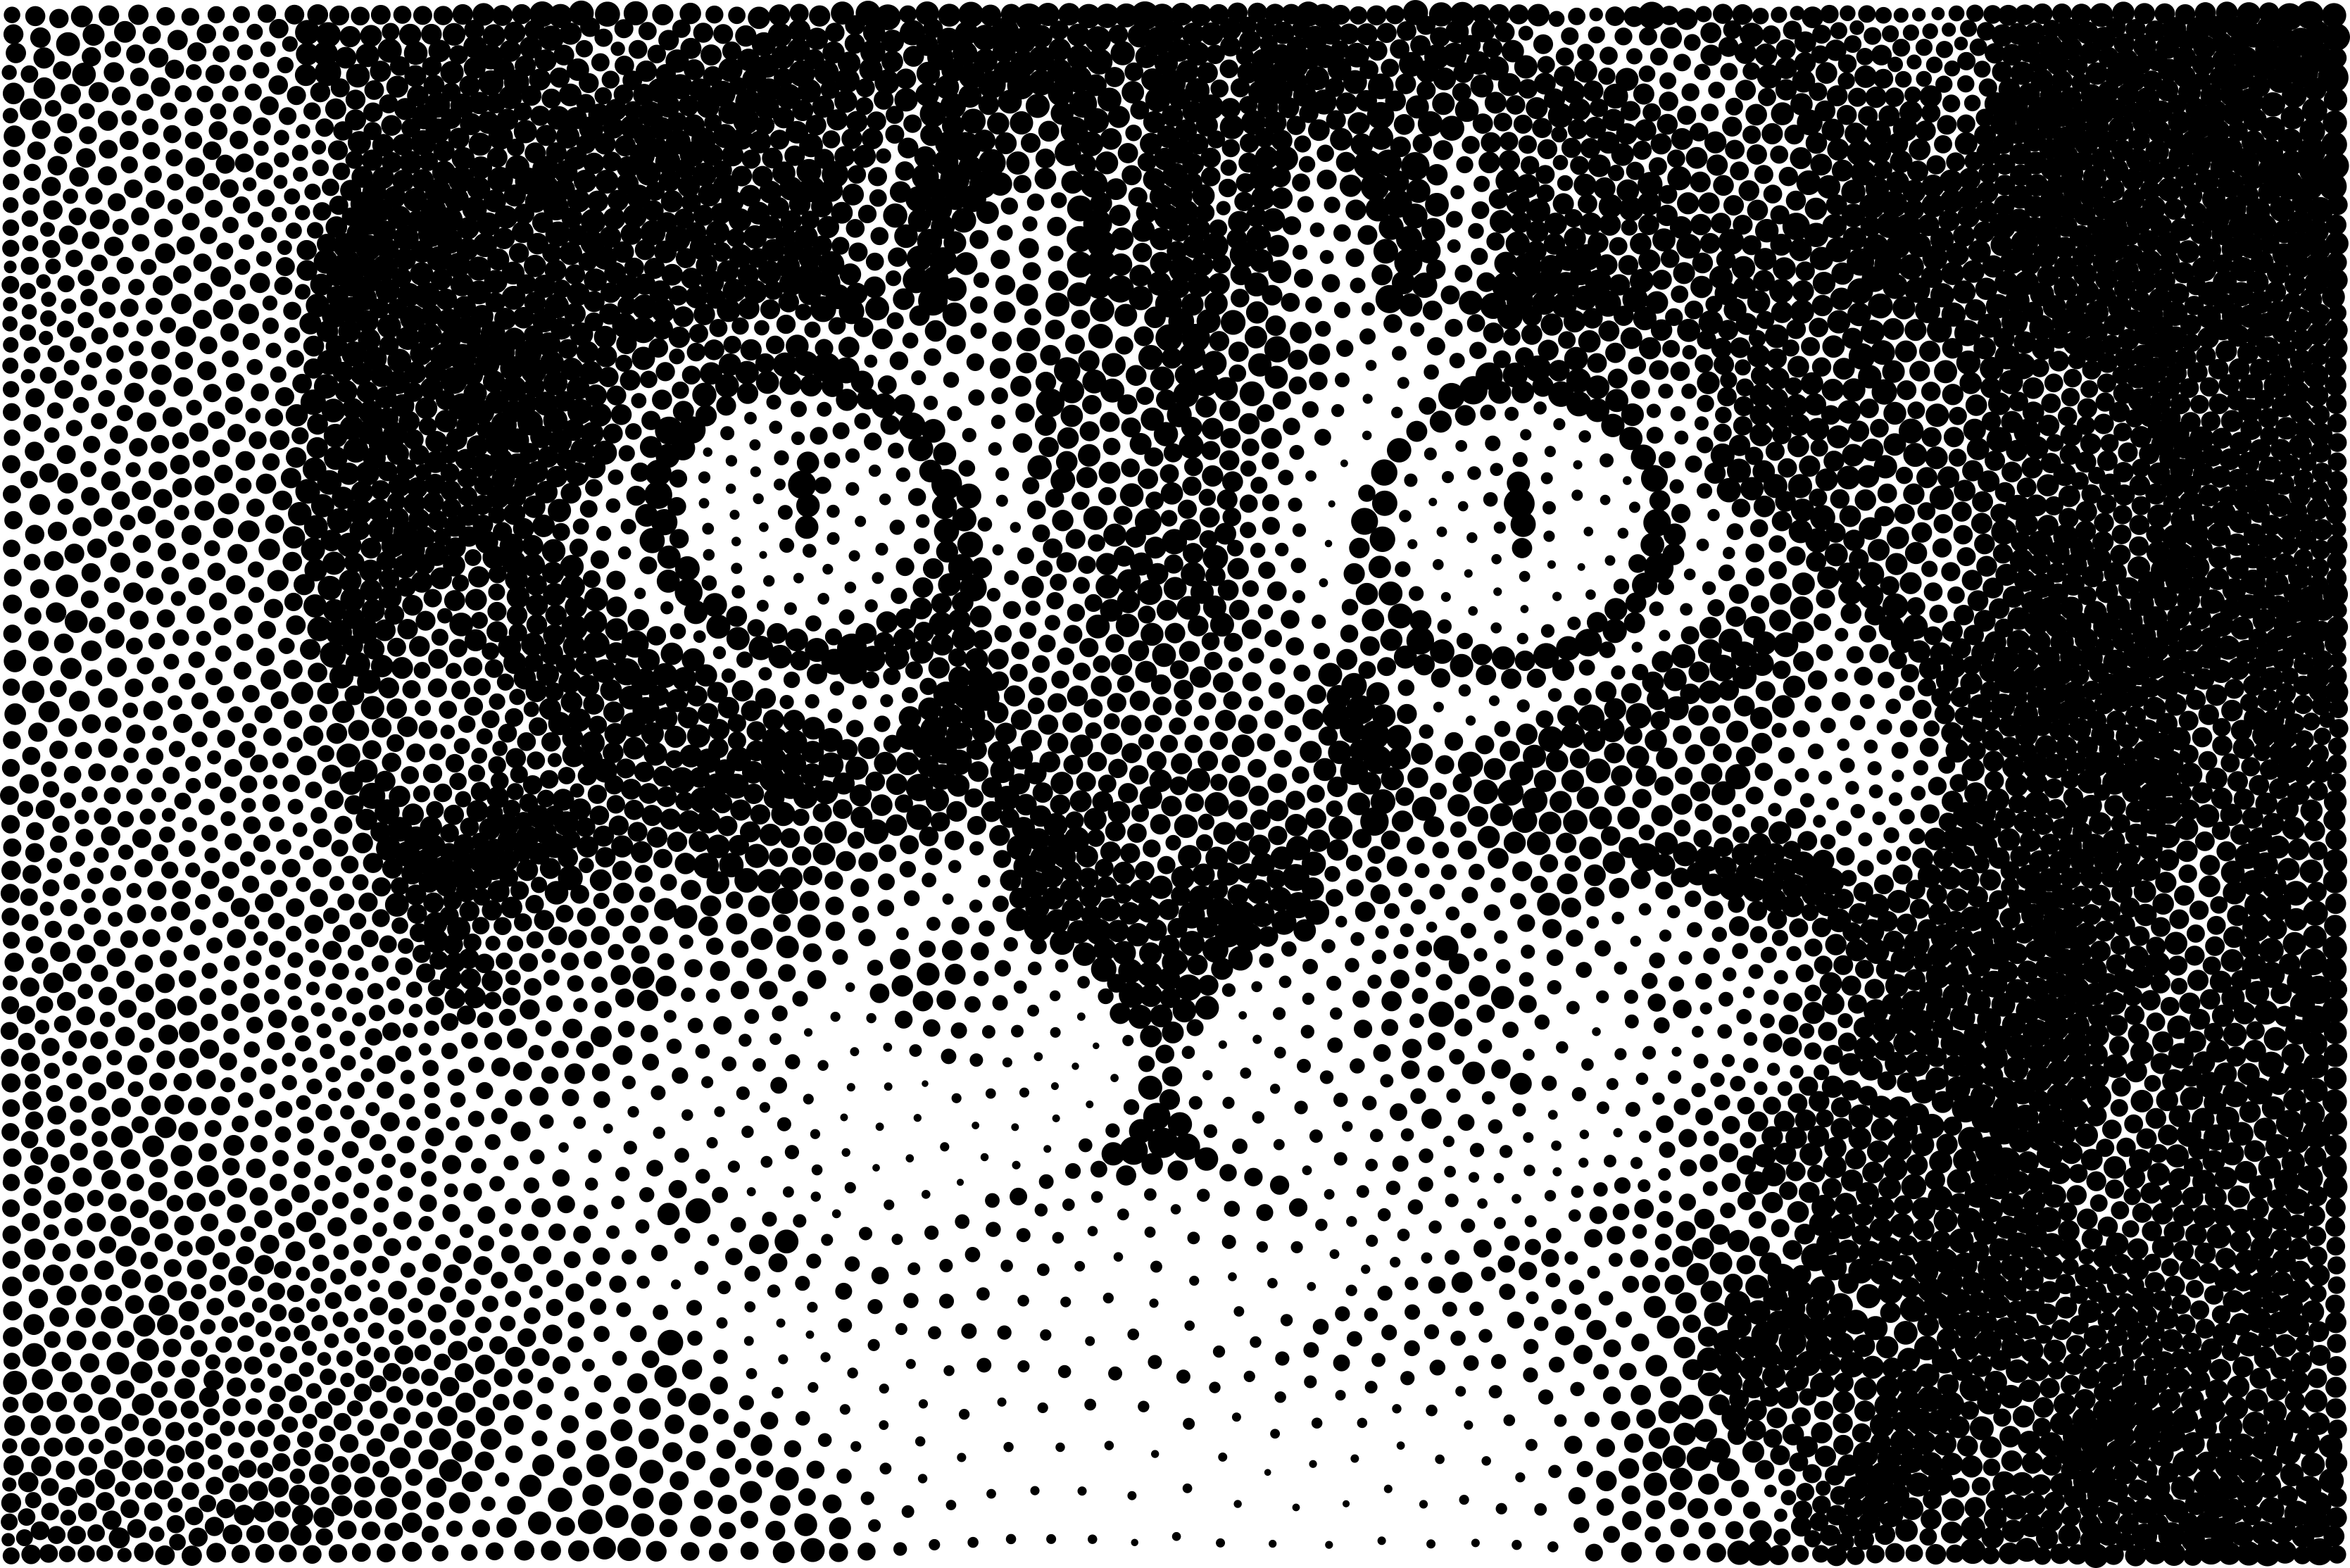
\includegraphics[width=0.22\textwidth]{FIGS/size/cat-middle-stippler.png}
    \label{fig:cat_s}
  }\hspace{-3mm}
  \subfigure[]{
    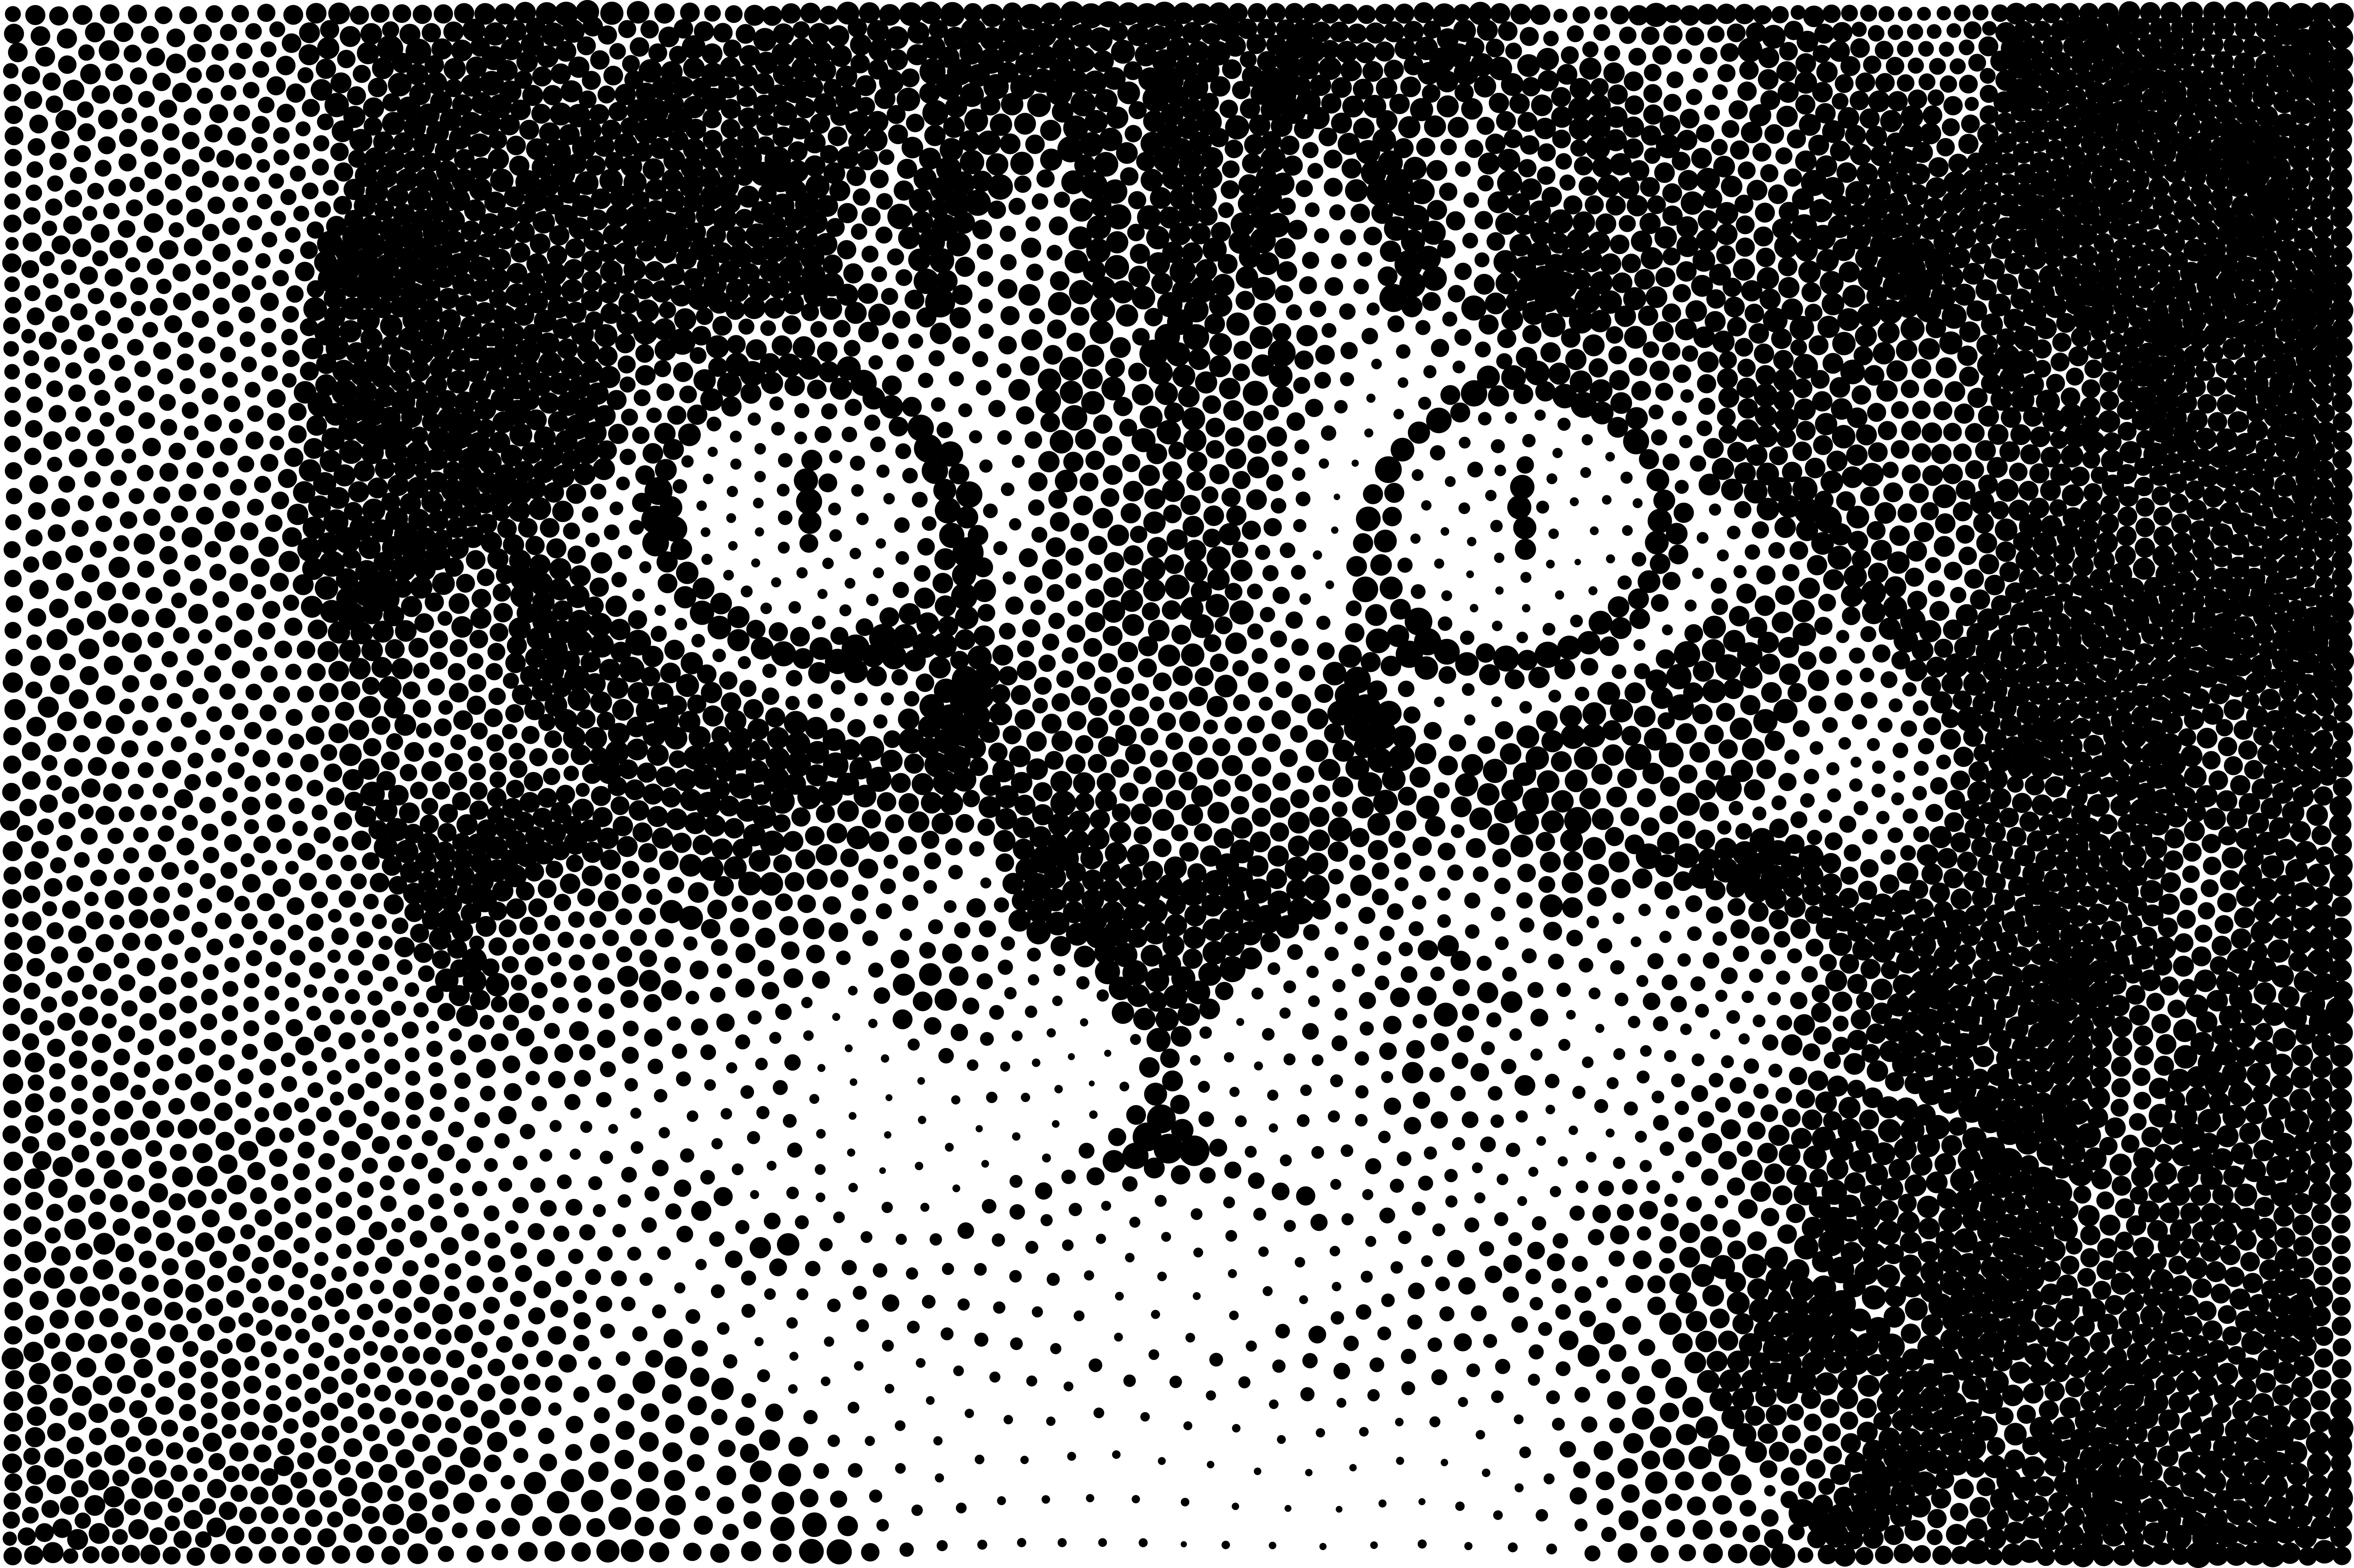
\includegraphics[width=0.22\textwidth]{FIGS/size/cat-large-stippler.png}
    \label{fig:cat_s}
  }
   \caption{The output result of both methods with various size of input image. The first row is the result of hedcuter method, and the second row is the result of voronoi method. \label{fig:cat_size}}
\end{figure*}
%%%%%%%%%%%%%%%%%%%%%%%%%%%%%%%%%%%%%%%%%%%%%%%%%%%%%%%%%%%%%%%%%%%%%%%%%%%%%%%%%%%%%%%%%%%%%%%%%%%%%%%%%%%
\subsection{the number of disks}
For both cases, if the number of disks increases, the result shows a tendency to draw details of original image. In Fig. \ref{fig:cat_numdisks}, features such as the head of squirrel in hedcut method and the tail of squirrel in voronoi method(marked by blue square) shows increase of detail. One disadvantage of increasing initial samples is lower time performance(Fig. \ref{fig:num_time}). There is a linear increase in time with the number of disks. Voronoi method shows the decrease of time with the number of disks because it uses multi-processing technique(Open MP) when it computes the tile and moves the sites. The area of each cell becomes smaller when the number of samples increases. Multiple smaller tasks advantage of parallel computation.
\begin{figure*}[hbt]
 \centering
 \subfigure[]{
    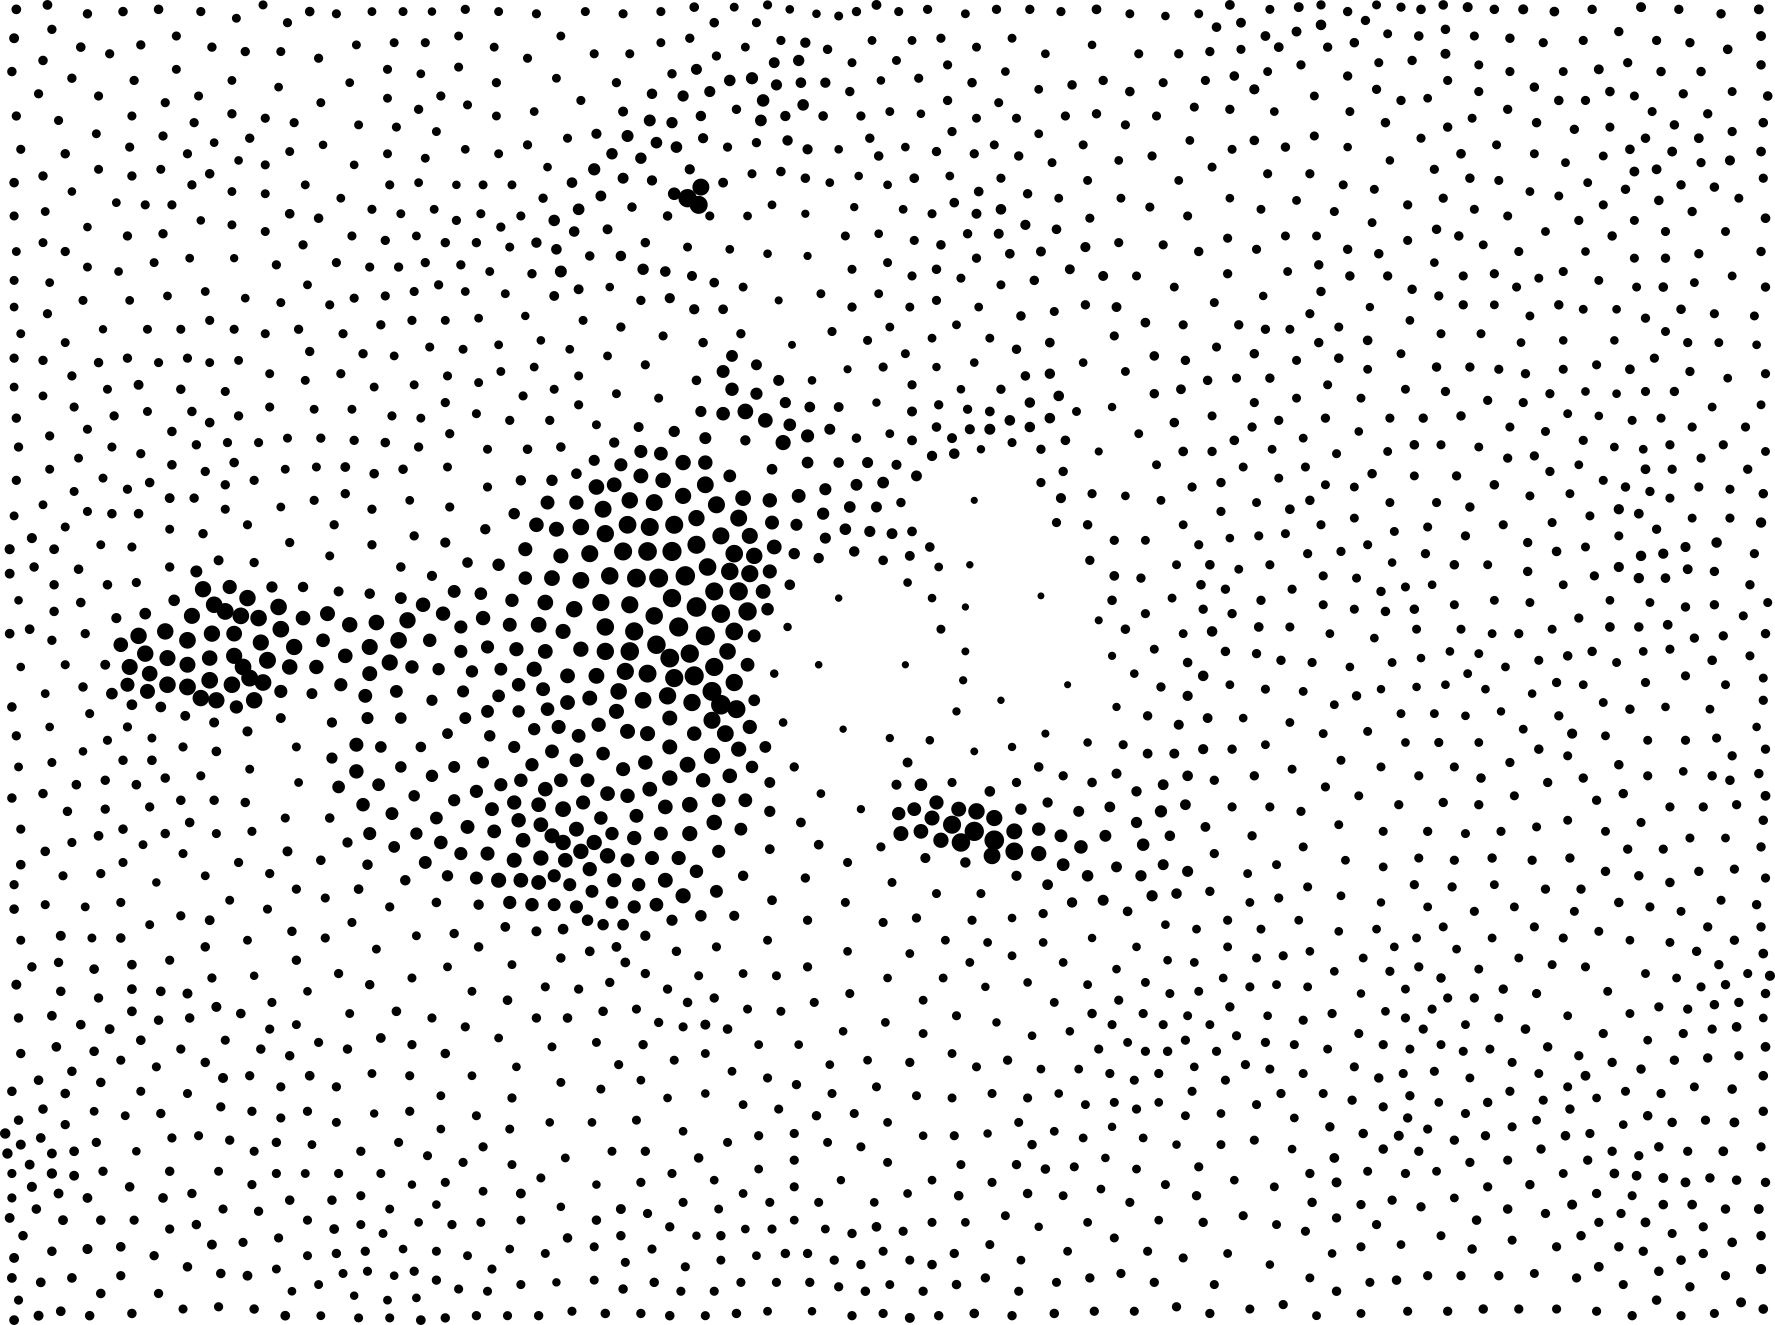
\includegraphics[width=0.32\textwidth]{FIGS/num/squirrel-2500.png}
    \label{fig:squirrel_2500-h}
  }\hspace{-3mm}
  \subfigure[]{
    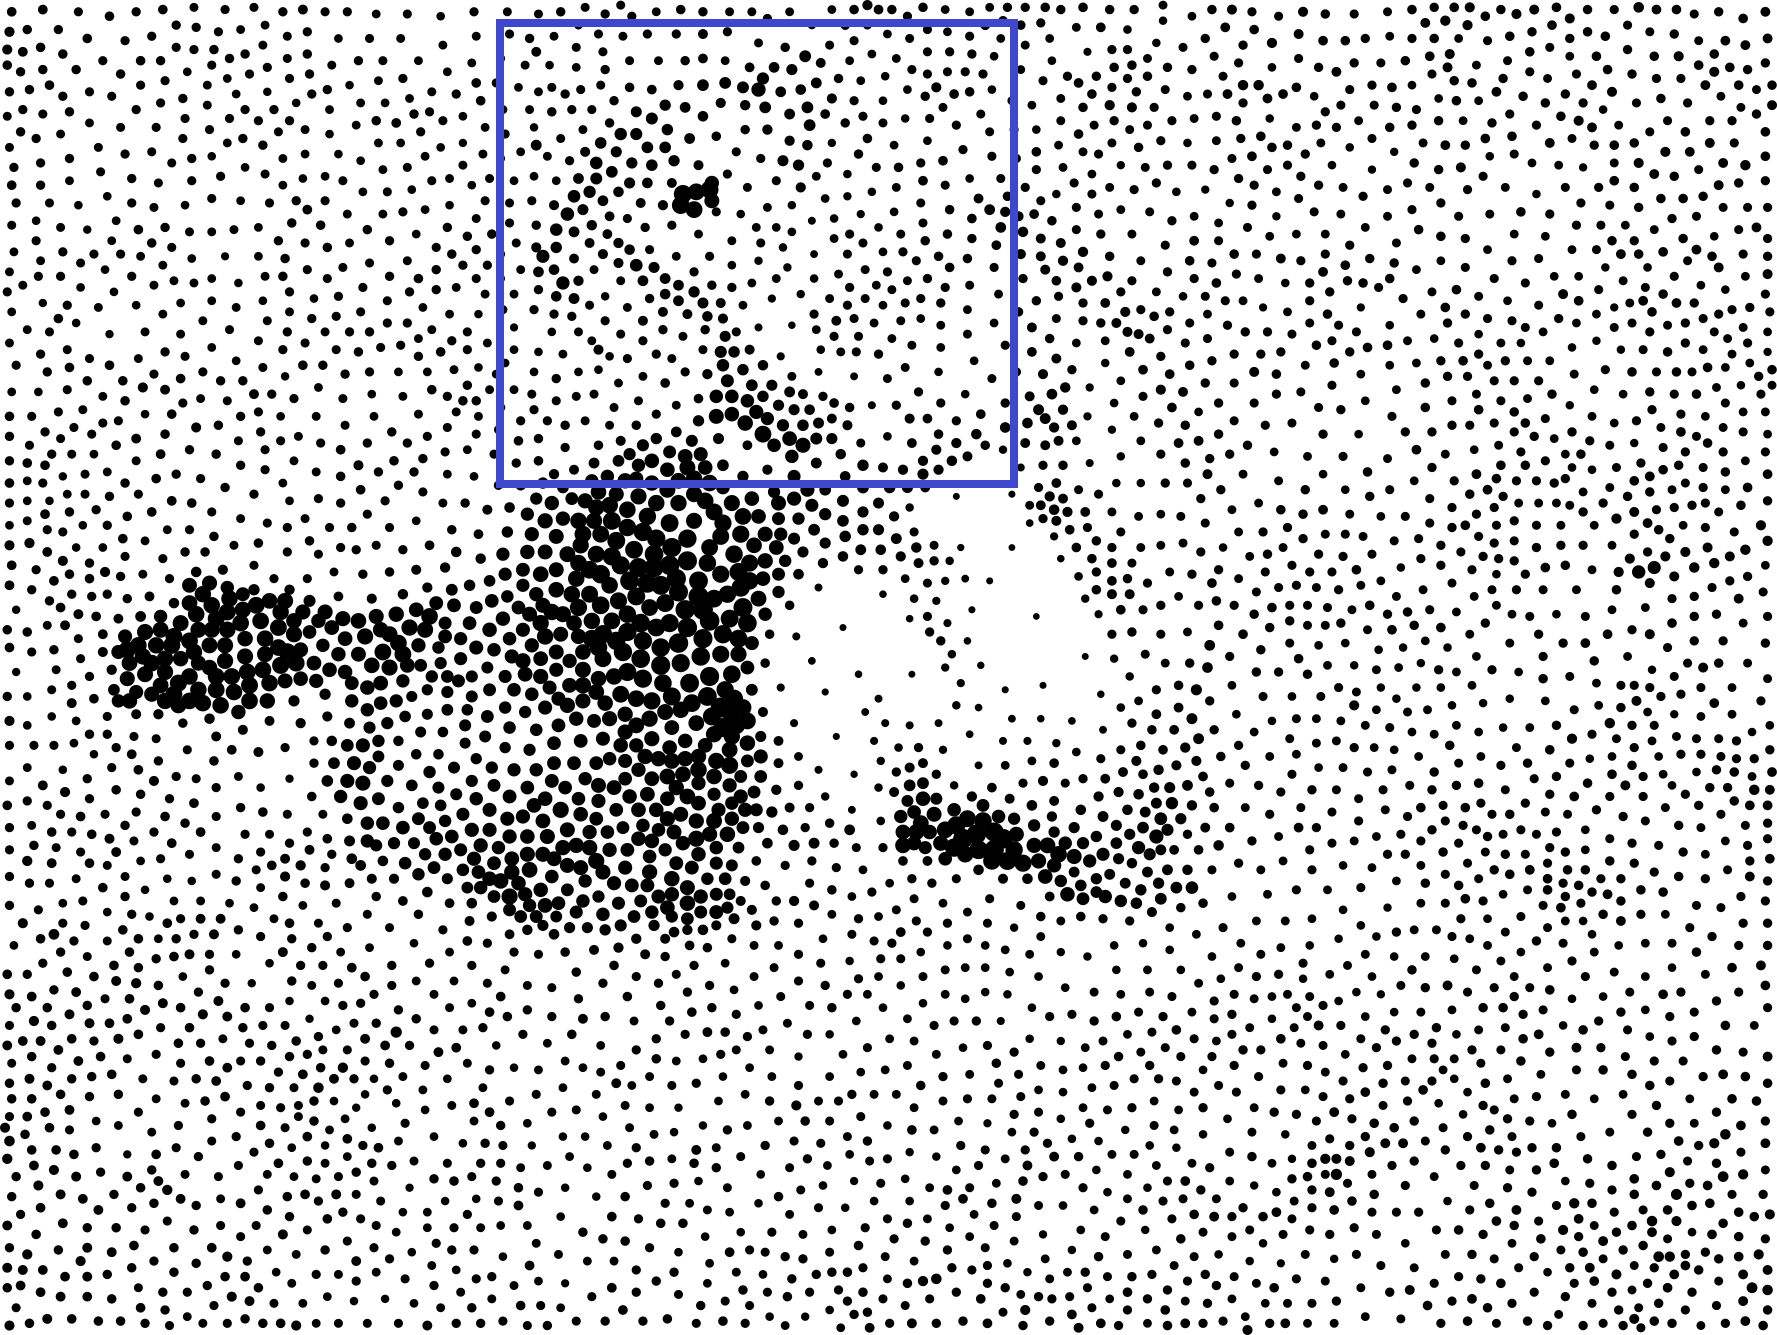
\includegraphics[width=0.32\textwidth]{FIGS/num/squirrel-5000.png}
    \label{fig:squirrel_5000-h}
  }\hspace{-3mm}
  \subfigure[]{
    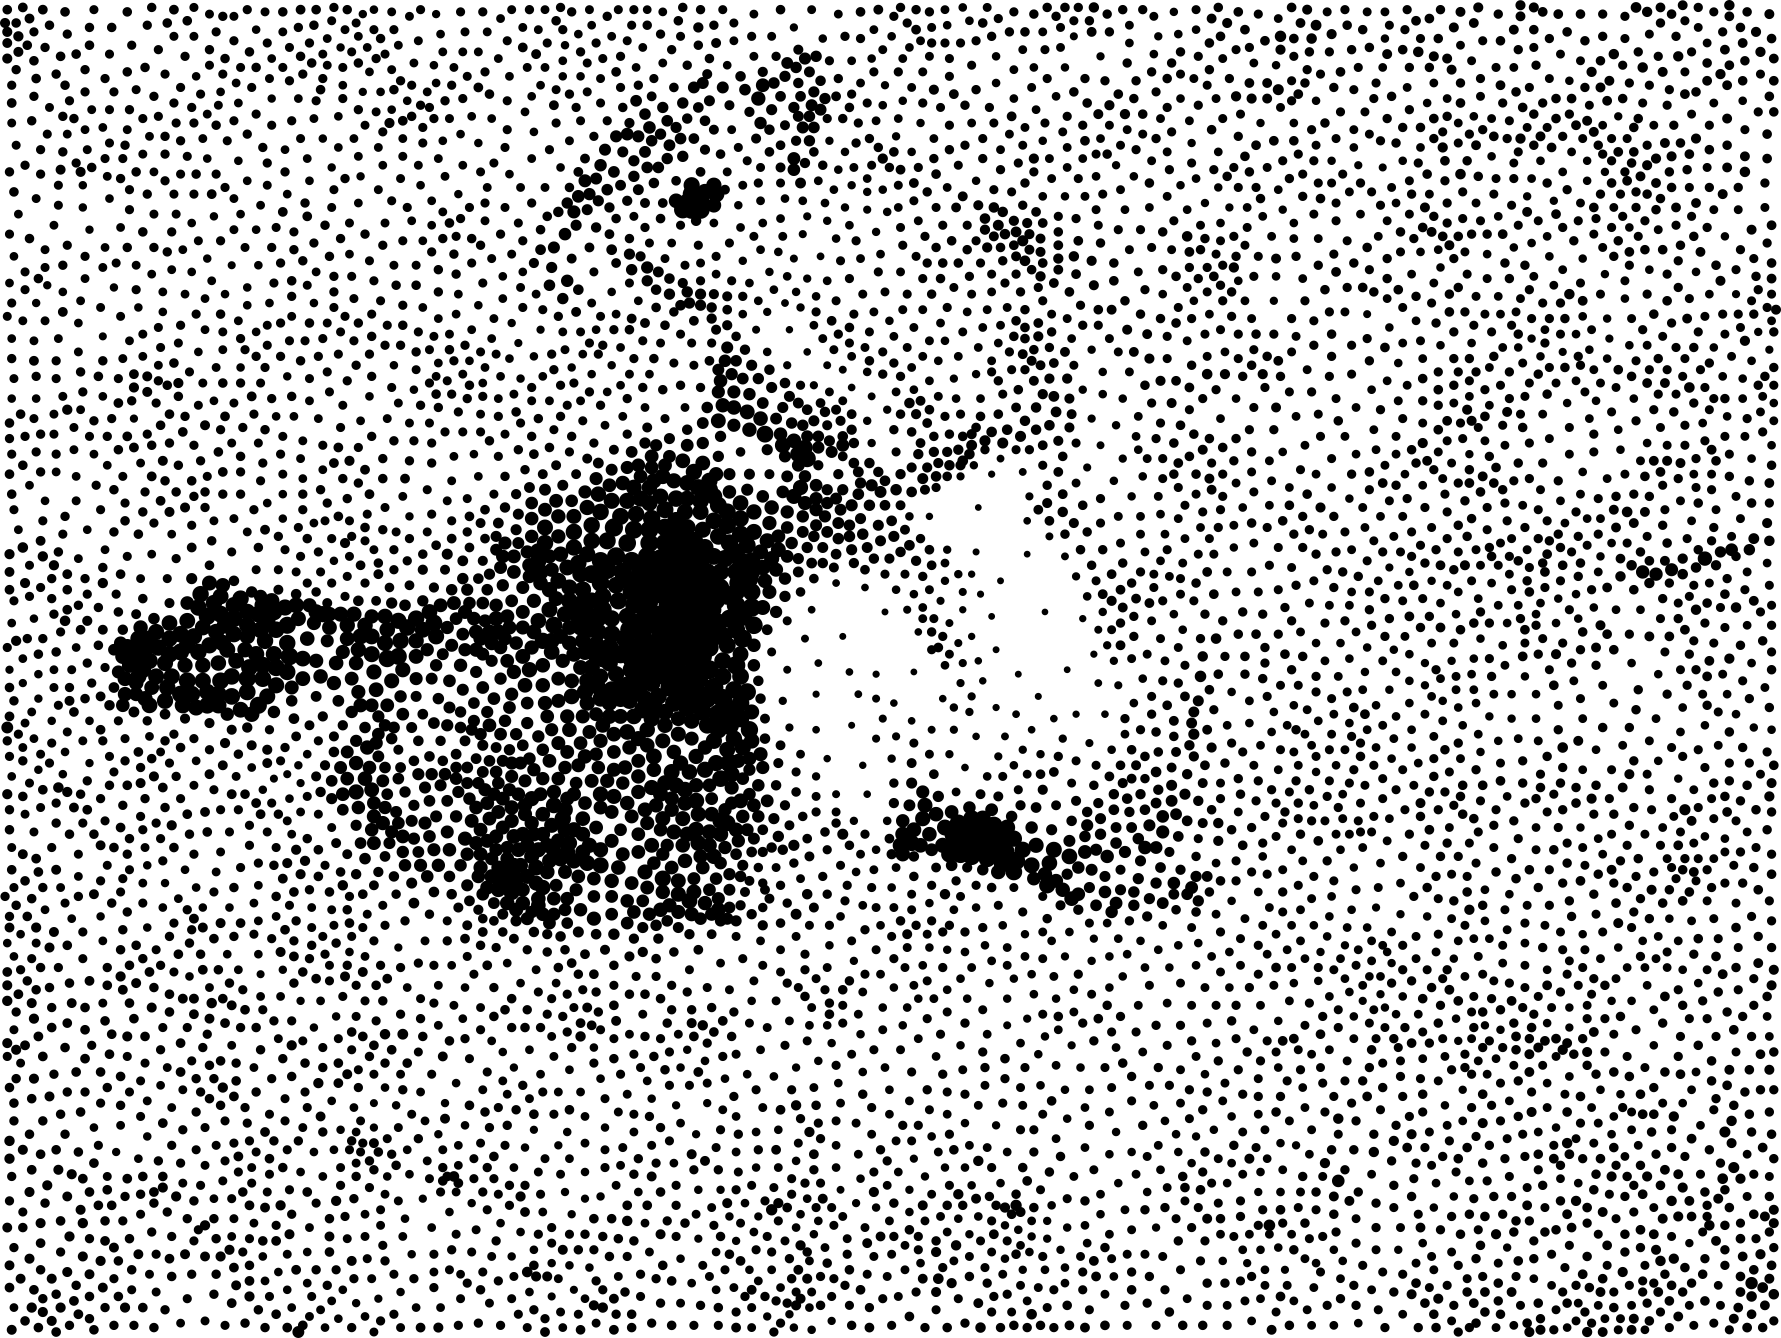
\includegraphics[width=0.32\textwidth]{FIGS/num/squirrel-7500.png}
    \label{fig:squirrel_7500-h}
  }\\
  \subfigure[]{
    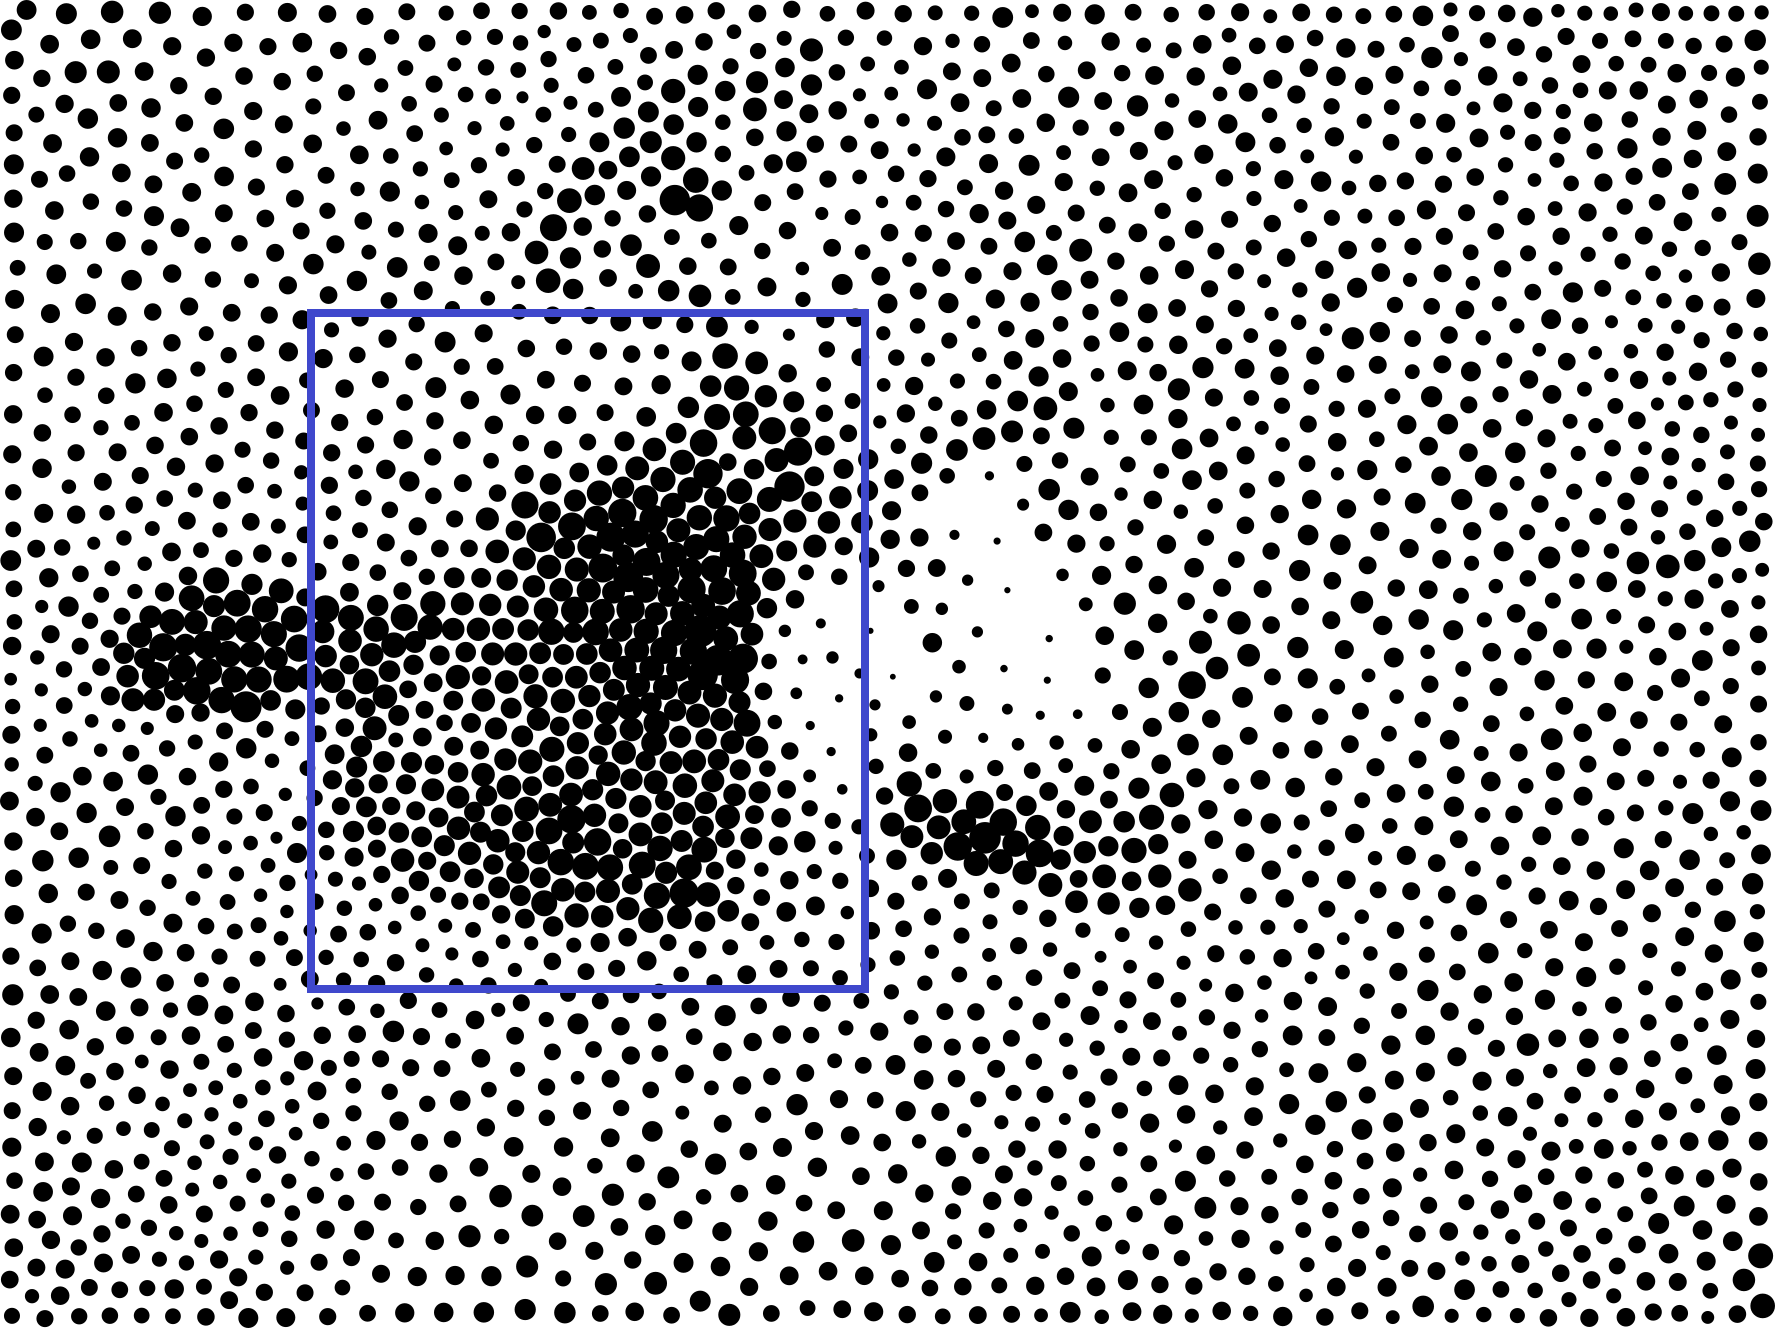
\includegraphics[width=0.32\textwidth]{FIGS/num/squirrel-2500-stippler.png}
    \label{fig:squirrel_2500-v}
  }\hspace{-3mm}
  \subfigure[]{
    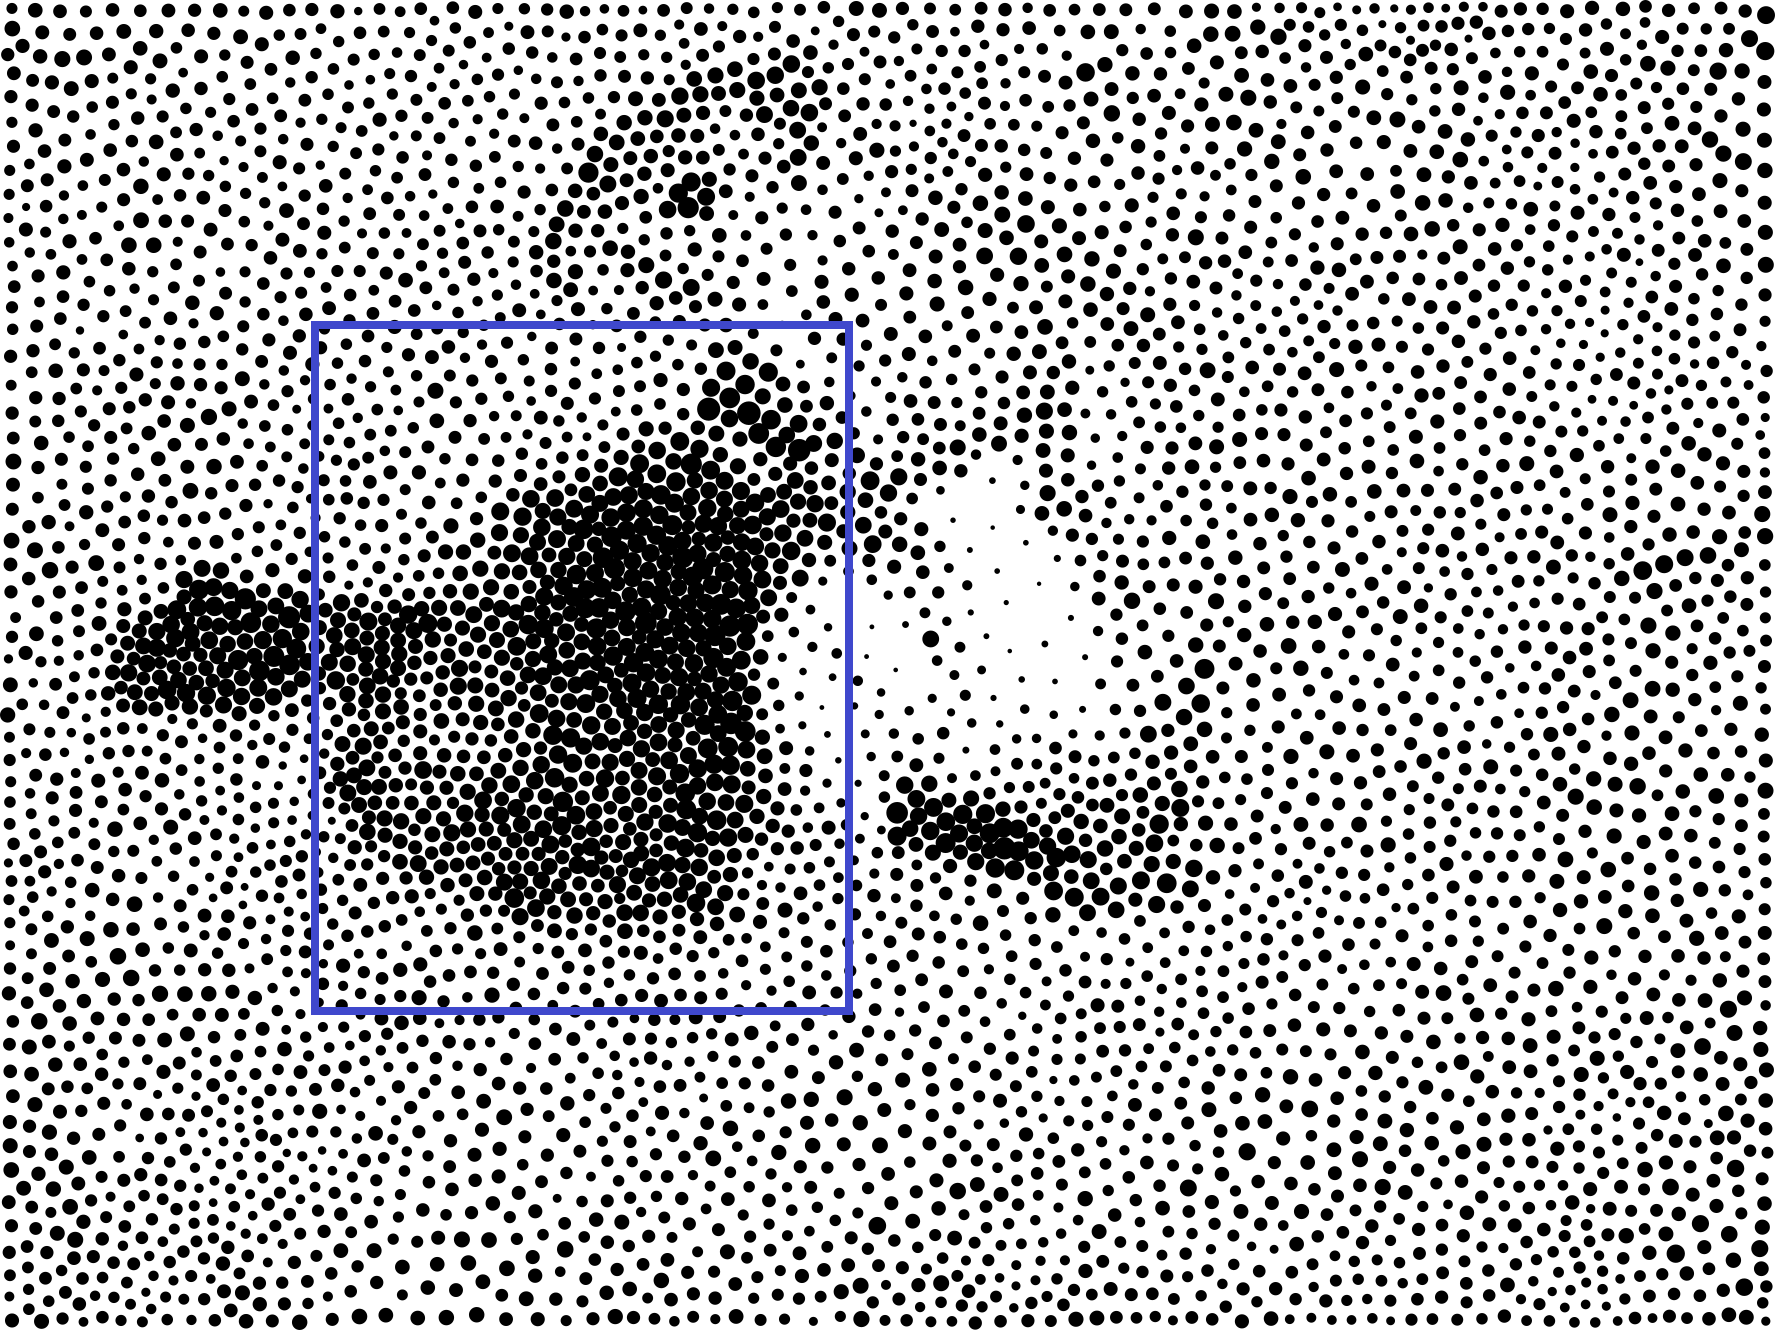
\includegraphics[width=0.32\textwidth]{FIGS/num/squirrel-5000-stippler.png}
    \label{fig:squirrel_5000-v}
  }\hspace{-3mm}
  \subfigure[]{
    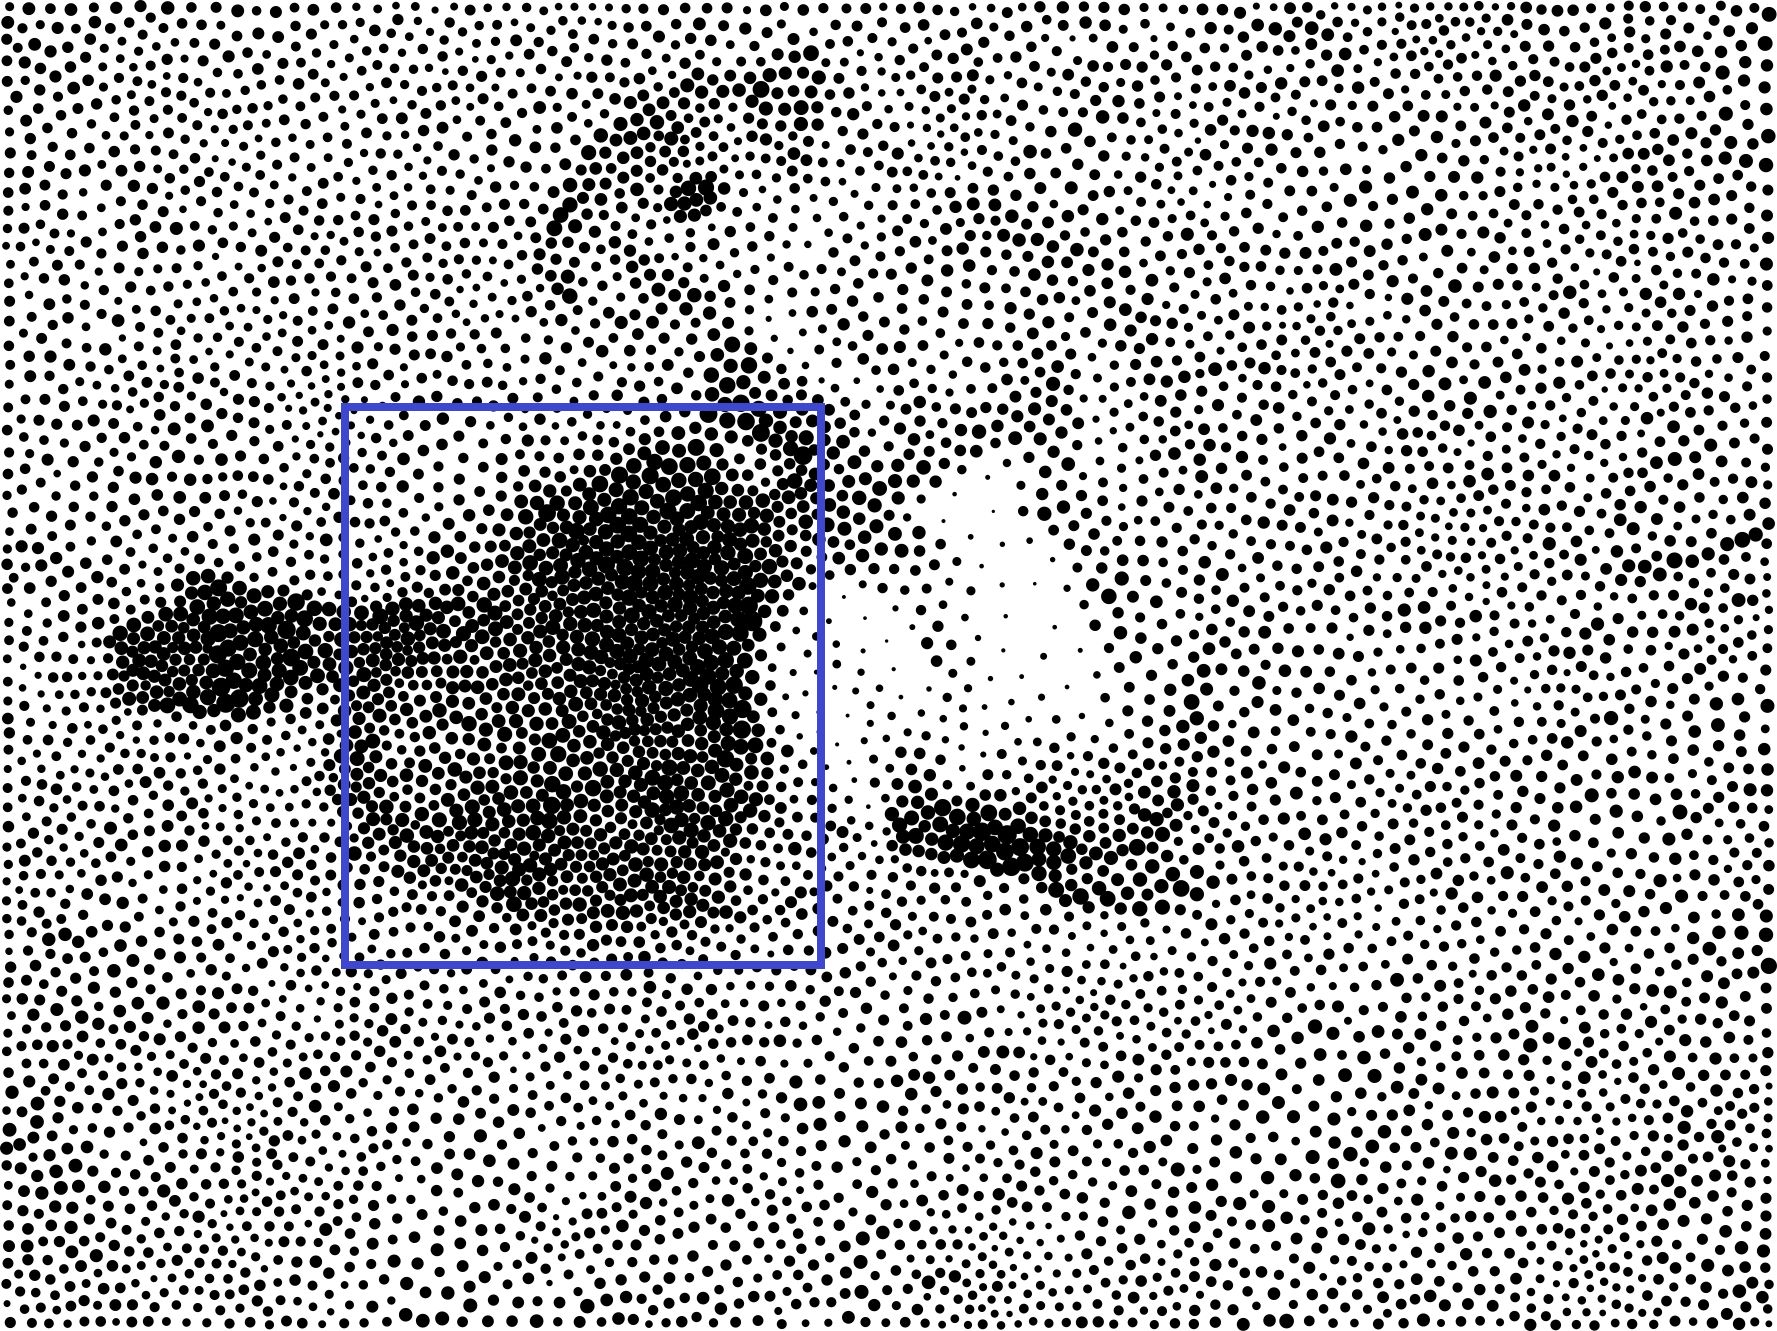
\includegraphics[width=0.32\textwidth]{FIGS/num/squirrel-7500-stippler.png}
    \label{fig:squirrel_7500-v}
  }
    \caption{The output results of different number of disks. From top row is the results of hedcuter method, and bottom row is the results of voronoi method. \label{fig:cat_numdisks}}
\end{figure*}
\begin{figure*}[hbt]
 \centering
 \subfigure[]{
    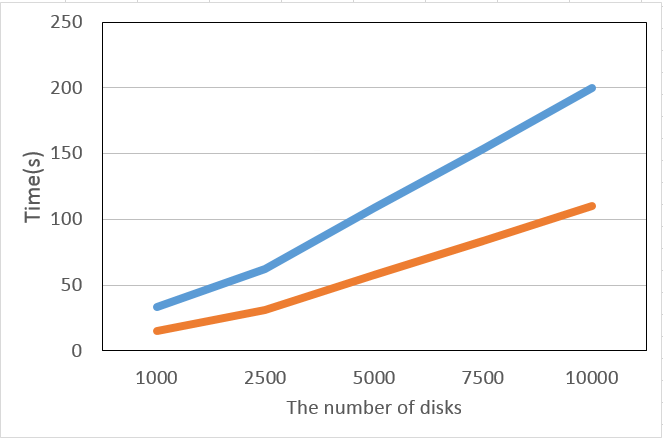
\includegraphics[width=0.42\textwidth]{FIGS/performance/hedcuter_erinking_che.png}
    \label{fig:time_h}
  }\hspace{-3mm}
  \subfigure[]{
    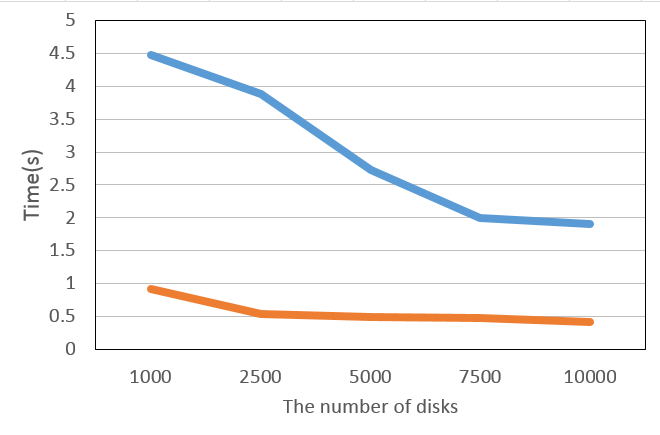
\includegraphics[width=0.42\textwidth]{FIGS/performance/voronoi_erinking_che.png}
    \label{fig:time_v}
  }
    \caption{The time performance of different number of disks. The left graph belongs to hedcuter method and the right graph belongs to voronoi method. The orange line is the result with Fig. \ref{fig:simple_erinking1} and the blue line is the result with Fig. \ref{fig:simple_che1}. \label{fig:num_time}}
\end{figure*}
%%%%%%%%%%%%%%%%%%%%%%%%%%%%%%%%%%%%%%%%%%%%%%%%%%%%%%%%%%%%%%%%%%%%%%%%%%%%%%%%%%%%%%%%%%%%%%%%%%%%%%%%%%%
\subsection{brightness of image}
The result of different brightness is shown in Fig. \ref{fig:cat_brightness}. From the first column to the last column, the brightness of image is -40\%, -20\%, +20\%, and 40\% of original image in order. Generally if the input image goes brighter, its stippling result seems to draw the input image more clear. For example, the left side of cat's face(marked by blue square) distinguishes clearly from the background as the input image goes brighter. Whiskers of the cat are also good example. However, it is worth noticing that brightness can remove some important features such as the lower jaw of the cat(marked by red square, Fig. \ref{fig:cat_b+40-h}, \ref{fig:cat_b+20-v}, and \ref{fig:cat_b+40-v}). This is because features are blurred with brightness in the input image, not because of algorithm itself. 
\begin{figure*}[hbt]
 \centering
 \subfigure[]{
    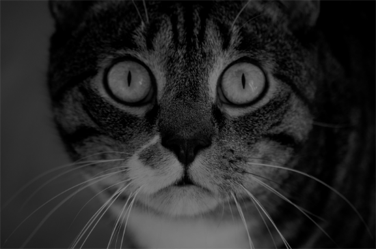
\includegraphics[width=0.22\textwidth]{FIGS/brightness/cat-b-40.png}
    \label{fig:cat_b-40}
  }\hspace{-3mm}
  \subfigure[]{
    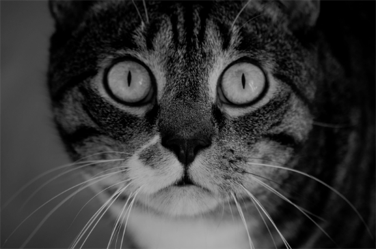
\includegraphics[width=0.22\textwidth]{FIGS/brightness/cat-b-20.png}
    \label{fig:cat_b-20}
  }\hspace{-3mm}
  \subfigure[]{
    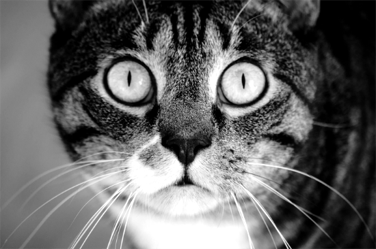
\includegraphics[width=0.22\textwidth]{FIGS/brightness/cat-b+20.png}
    \label{fig:cat_b+20}
  }\hspace{-3mm}
  \subfigure[]{
    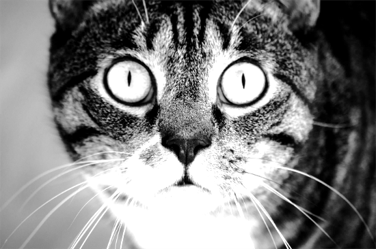
\includegraphics[width=0.22\textwidth]{FIGS/brightness/cat-b+40.png}
    \label{fig:cat_b+40}
  }\\
   \subfigure[]{
    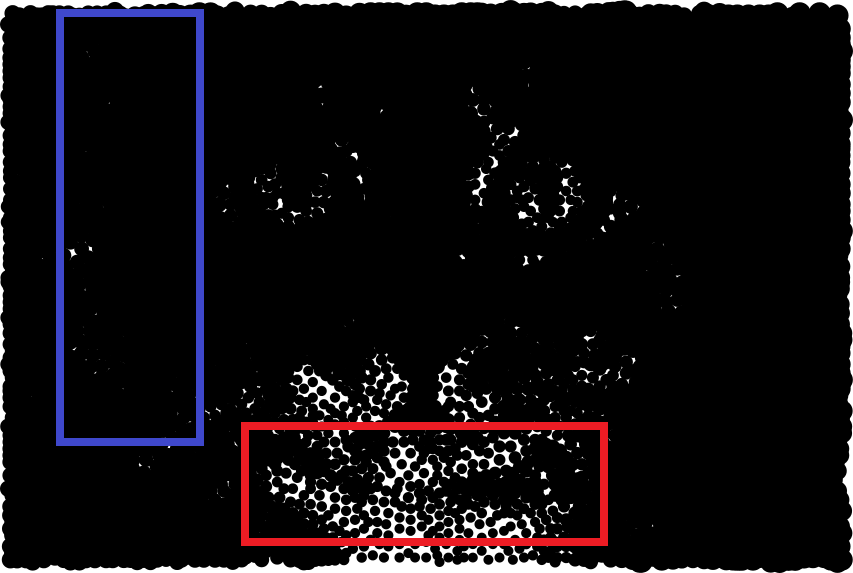
\includegraphics[width=0.22\textwidth]{FIGS/brightness/cat-b-40-7500.png}
    \label{fig:cat_b-40-h}
  }\hspace{-3mm}
  \subfigure[]{
    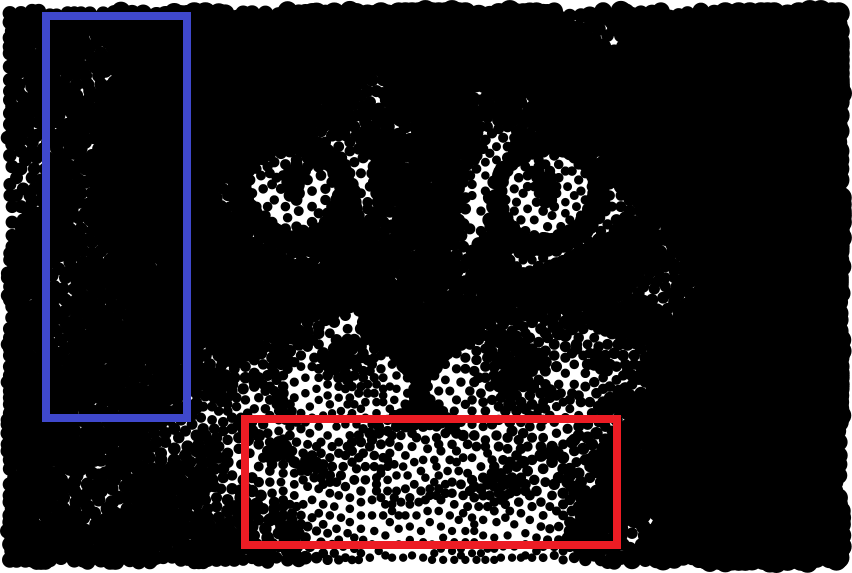
\includegraphics[width=0.22\textwidth]{FIGS/brightness/cat-b-20-7500.png}
    \label{fig:cat_b-20-h}
  }\hspace{-3mm}
  \subfigure[]{
    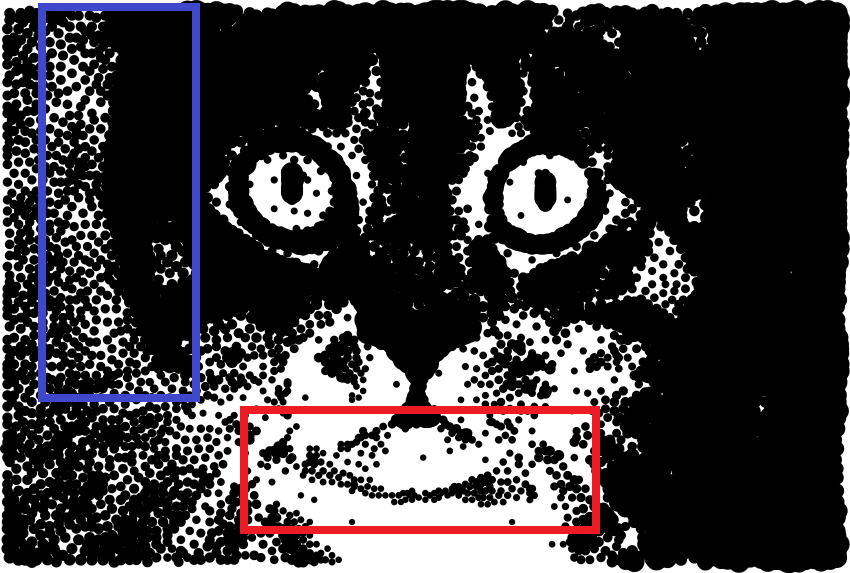
\includegraphics[width=0.22\textwidth]{FIGS/brightness/cat-b+20-7500.png}
    \label{fig:cat_b+20-h}
  }\hspace{-3mm}
  \subfigure[]{
    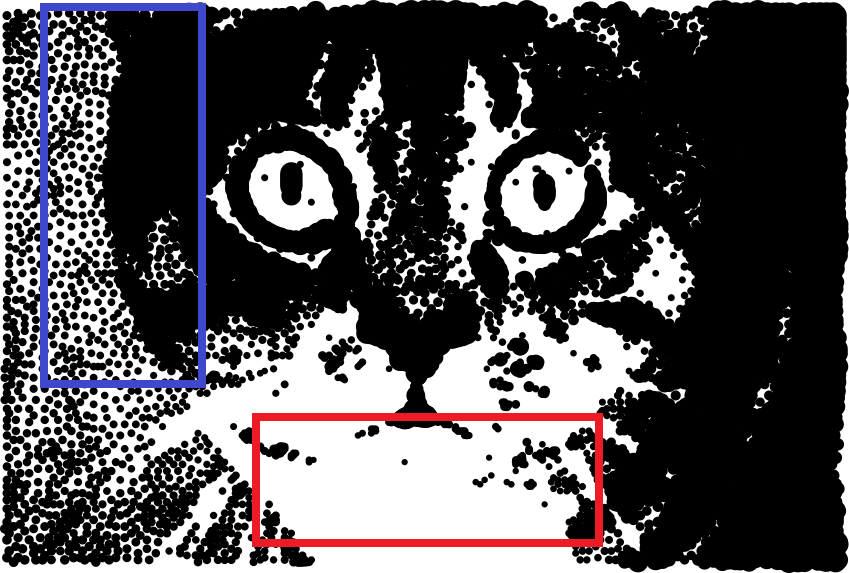
\includegraphics[width=0.22\textwidth]{FIGS/brightness/cat-b+40-7500.png}
    \label{fig:cat_b+40-h}
  }\\
   \subfigure[]{
    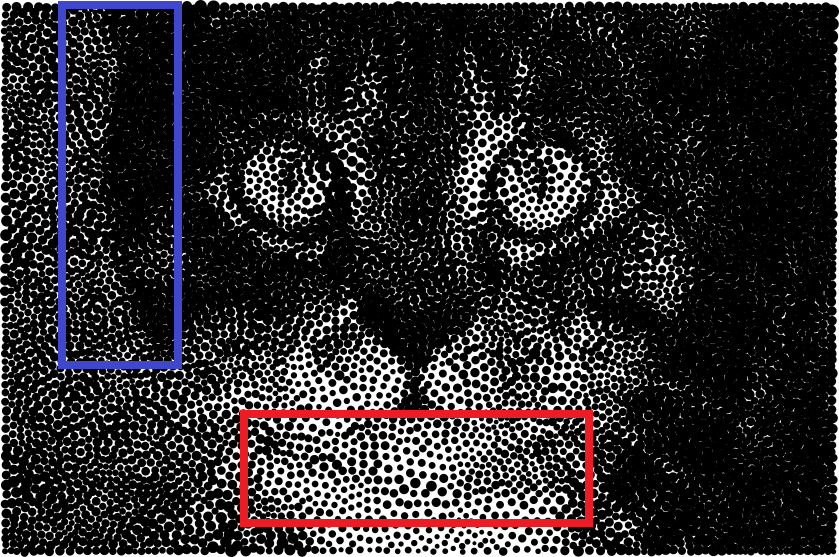
\includegraphics[width=0.22\textwidth]{FIGS/brightness/cat-b-40-stippler.png}
    \label{fig:cat_b-40-v}
  }\hspace{-3mm}
  \subfigure[]{
    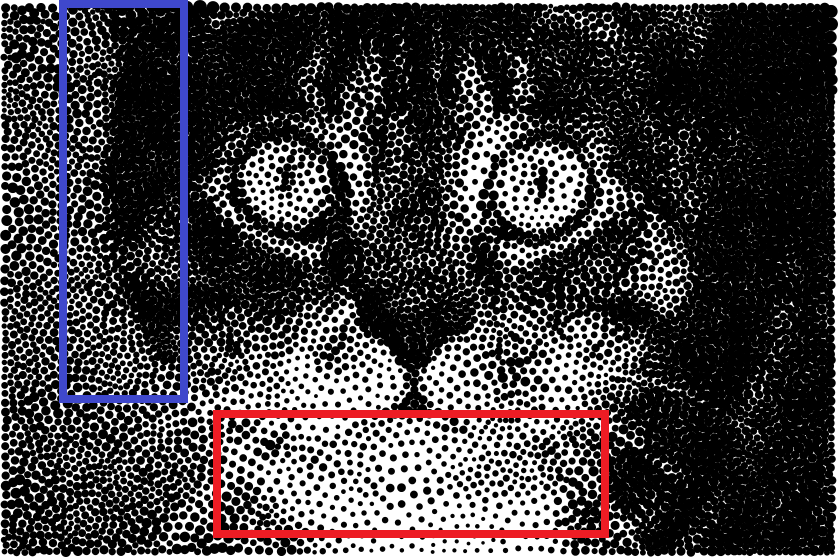
\includegraphics[width=0.22\textwidth]{FIGS/brightness/cat-b-20-stippler.png}
    \label{fig:cat_b-20-v}
  }\hspace{-3mm}
  \subfigure[]{
    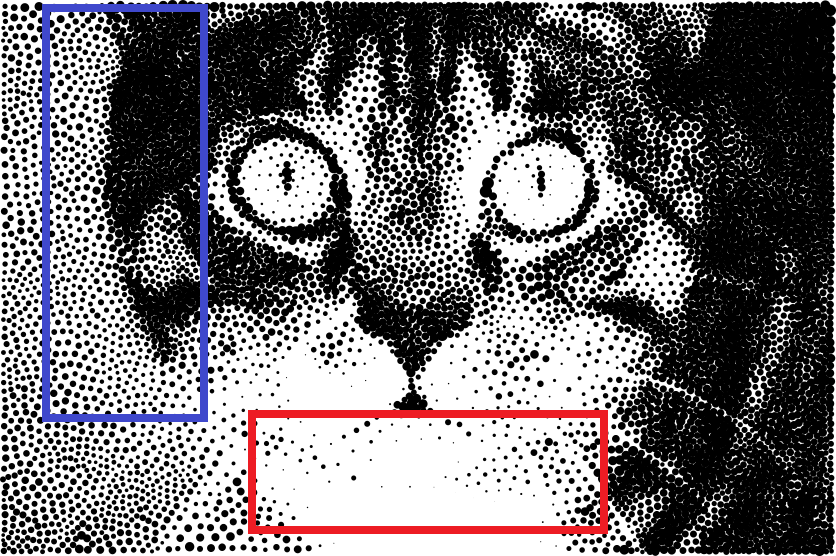
\includegraphics[width=0.22\textwidth]{FIGS/brightness/cat-b+20-stippler.png}
    \label{fig:cat_b+20-v}
  }\hspace{-3mm}
  \subfigure[]{
    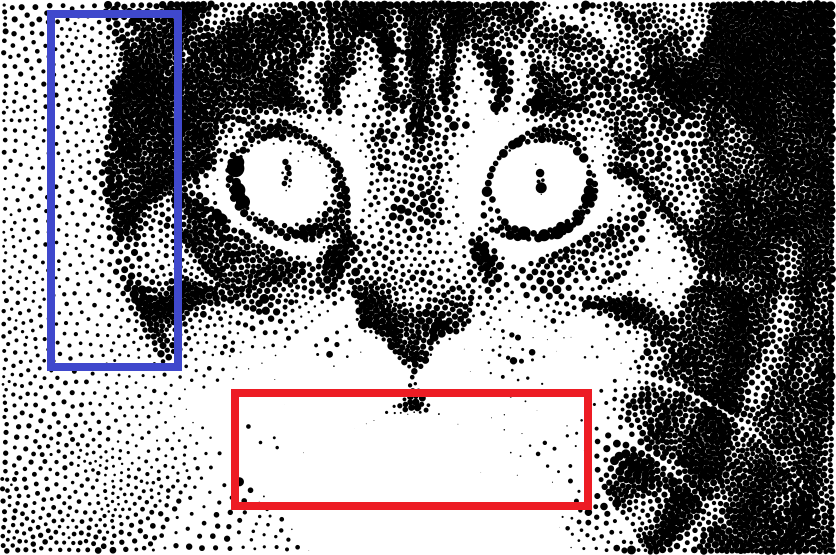
\includegraphics[width=0.22\textwidth]{FIGS/brightness/cat-b+40-stippler.png}
    \label{fig:cat_b+40-v}
  }\\
    \caption{The output results of different brightness. From top to bottom row, it shows input images, the results of hedcuter method, and the results of voronoi method. \label{fig:cat_brightness}}
\end{figure*}
%%%%%%%%%%%%%%%%%%%%%%%%%%%%%%%%%%%%%%%%%%%%%%%%%%%%%%%%%%%%%%%%%%%%%%%%%%%%%%%%%%%%%%%%%%%%%%%%%%%%%%%%%%%%
\subsection{contrast of image}
Following Fig. \ref{fig:cat_contrast} shows the result of contrast. From the left to the right, the level of contrast of each column is -40\%, -20\%, +20\% and +40\% of the original image. Features in various contrast of image also affected in different way like brightness. Some features are blurred and some features are distinct. For instance, cat's eye in hedcuter method and the left side of face in voronoi method(marked by blue square) shows strong contrast in stippling results also. However, the left side of face in hedcuter method and the patterns on forehead shows dimmer results(marked by red square) while contrast grows stronger. This causes unexpected result of stippling.
\begin{figure*}[hbt]
 \centering
 \subfigure[]{
    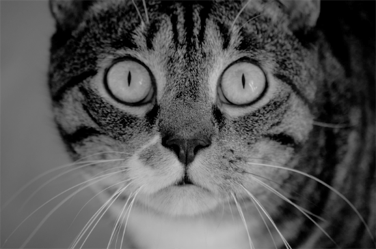
\includegraphics[width=0.22\textwidth]{FIGS/contrast/cat-c-40.png}
    \label{fig:cat_c-40}
  }\hspace{-3mm}
  \subfigure[]{
    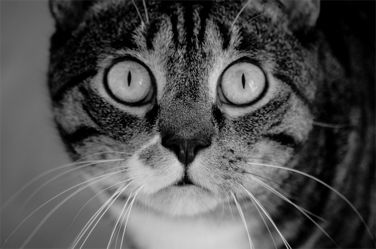
\includegraphics[width=0.22\textwidth]{FIGS/contrast/cat-c-20.png}
    \label{fig:cat_c-20}
  }\hspace{-3mm}
  \subfigure[]{
    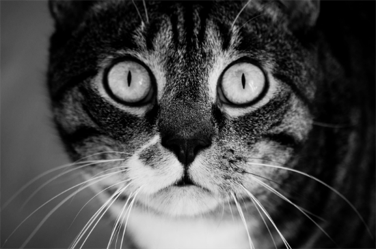
\includegraphics[width=0.22\textwidth]{FIGS/contrast/cat-c+20.png}
    \label{fig:cat_c+20}
  }\hspace{-3mm}
  \subfigure[]{
    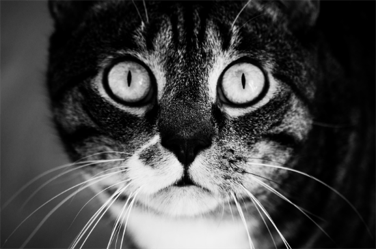
\includegraphics[width=0.22\textwidth]{FIGS/contrast/cat-c+40.png}
    \label{fig:cat_c+40}
  }\\
  \subfigure[]{
    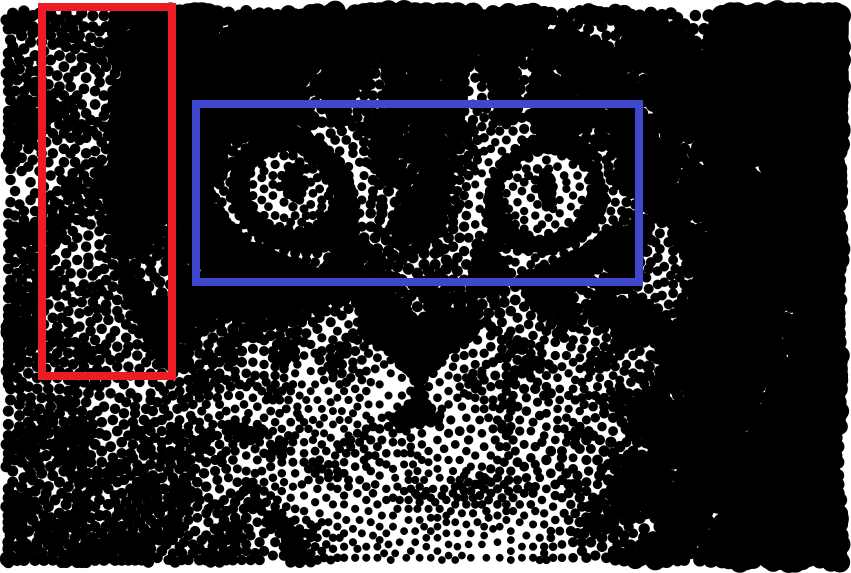
\includegraphics[width=0.22\textwidth]{FIGS/contrast/cat-c-40-7500.png}
    \label{fig:cat_c-40-h}
  }\hspace{-3mm}
  \subfigure[]{
    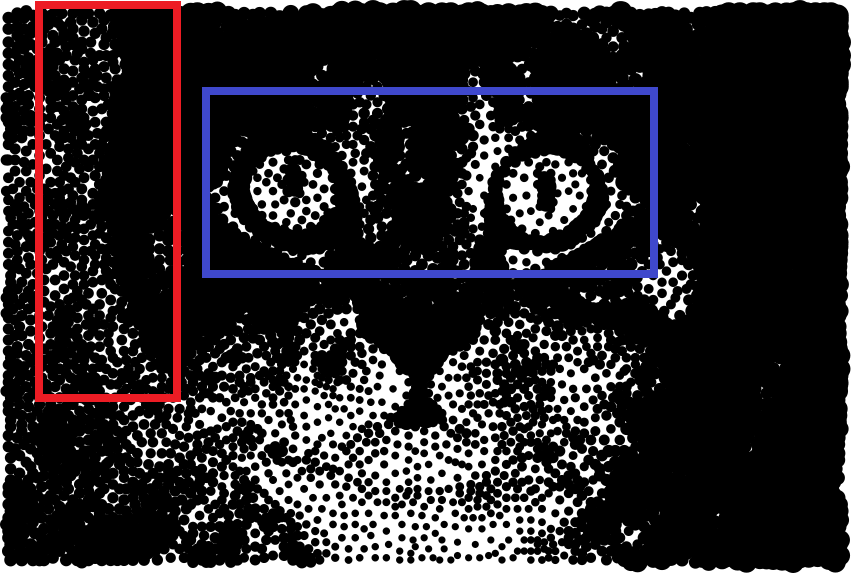
\includegraphics[width=0.22\textwidth]{FIGS/contrast/cat-c-20-7500.png}
    \label{fig:cat_c-20-h}
  }\hspace{-3mm}
  \subfigure[]{
    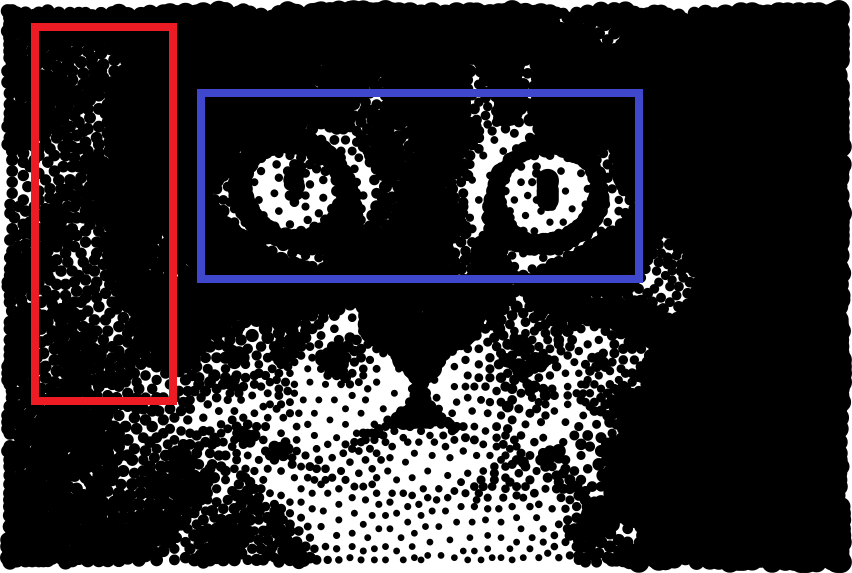
\includegraphics[width=0.22\textwidth]{FIGS/contrast/cat-c+20-7500.png}
    \label{fig:cat_c+20-h}
  }\hspace{-3mm}
  \subfigure[]{
    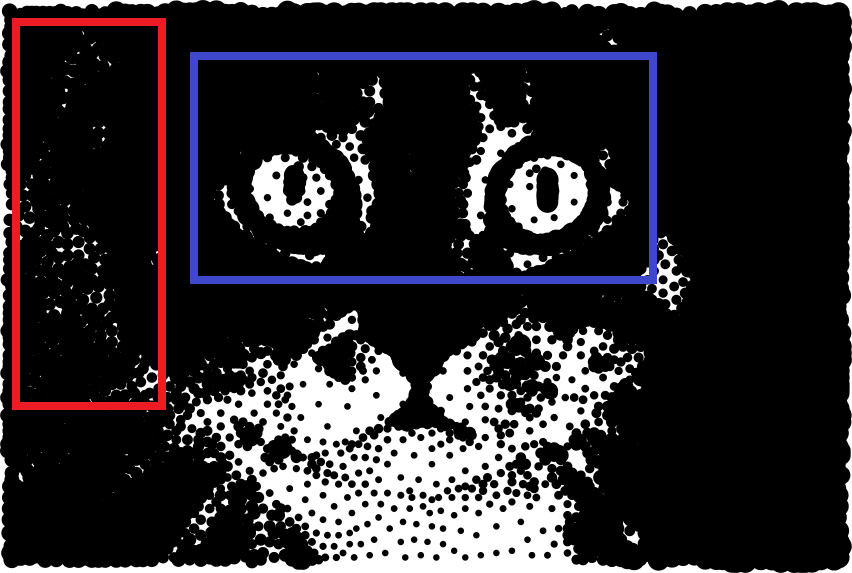
\includegraphics[width=0.22\textwidth]{FIGS/contrast/cat-c+40-7500.png}
    \label{fig:cat_c+40-h}
  }\\
  \subfigure[]{
    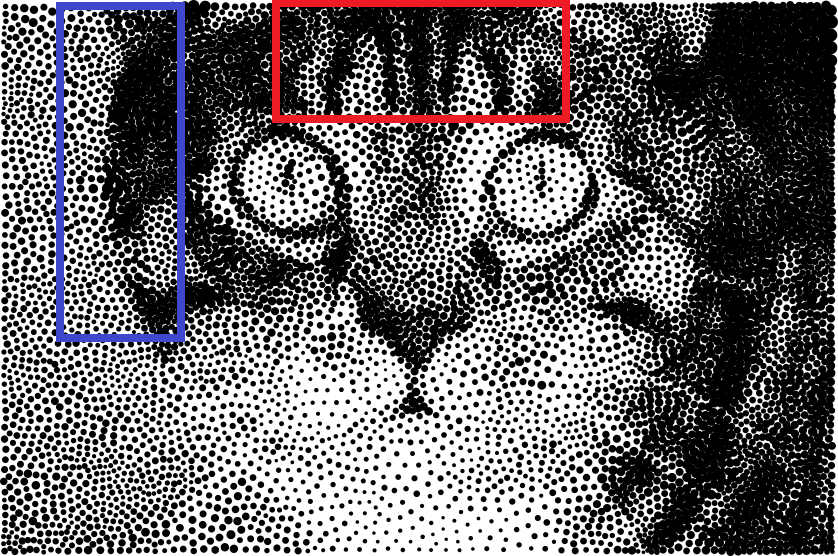
\includegraphics[width=0.22\textwidth]{FIGS/contrast/cat-c-40-stippler.png}
    \label{fig:cat_c-40-v}
  }\hspace{-3mm}
  \subfigure[]{
    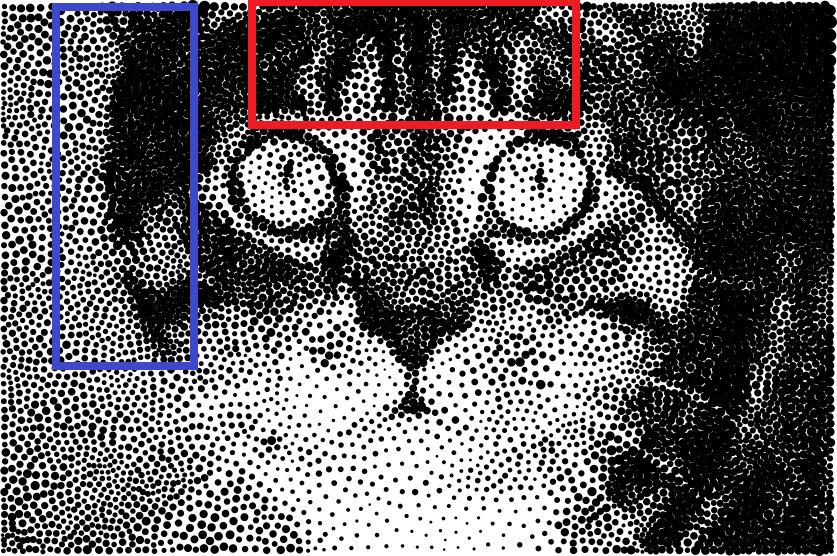
\includegraphics[width=0.22\textwidth]{FIGS/contrast/cat-c-20-stippler.png}
    \label{fig:cat_c-20-v}
  }\hspace{-3mm}
  \subfigure[]{
    \includegraphics[width=0.22\textwidth]{FIGS/contrast/cat-c+20-stippler.png}
    \label{fig:cat_c+20-v}
  }\hspace{-3mm}
  \subfigure[]{
    \includegraphics[width=0.22\textwidth]{FIGS/contrast/cat-c+40-stippler.png}
    \label{fig:cat_c+40-v}
  }\\
    \caption{The output results of different contrast. From top to bottom row, it shows input images, the results of hedcuter method, and the results of voronoi method. \label{fig:cat_contrast}}
\end{figure*}
%%%%%%%%%%%%%%%%%%%%%%%%%%%%%%%%%%%%%%%%%%%%%%%%%%%%%%%%%%%%%%%%%%%%%%%%%%%%%%%%%%%%%%%%%%%%%%%%%%%%%%%%%%%%
\section{Improvement of hedcuter method}
\subsection{distribution}
Based on observation in Sec. \ref{outputs}, I concluded that the size of image can improve distributions. The number of disks also can improve distribution, but in hedcuter method case, it has linear increase in time without any acceleration technique. Brightness and contrast are uncontrollable, because some features are removed. Therefore I used subpixels to make virtual resolution image suggested in assignment paper.\\
The first step is to create high-resolution image of input when construction of voronoi diagram starts and map the sites to virtual image. Next the algorithm computes intensities based on virtual image with wider voronoi region and computes the new centroids. These cenetroids are mapped to original resolution. Here are results of simple gradient image with subpixels in Fig.\ref{fig:subpixels}. It connect to the option \textbf{-subpixels [num]}.\\
In first and second examples(rows) in Fig. \ref{fig:subpixels}, it hard to recognize how voids and clustering is reduced. In order to observed in detail, I made the third examples. It shows that when the number of subpixels increase, the top boundary reduces the clustering(marked by blue square). But the result shows that clustering still exists in Fig. \ref{fig:test_subpixel10} and it shows no improvement on distribution over the certain number of subpixels. Also if I increase the size of virtual resolution image, it need more time to compute the results. 
\begin{figure*}[hbt]
 \centering
   \subfigure[]{
    \includegraphics[width=0.22\textwidth]{FIGS/subpixels/Hurst.png}
    \label{fig:hurst-original}
  }\hspace{-3mm}
  \subfigure[]{
    \includegraphics[width=0.22\textwidth]{FIGS/subpixels/Hurst-5000.png}
    \label{fig:hurst-subpixel1}
  }\hspace{-3mm}
    \subfigure[]{
    \includegraphics[width=0.22\textwidth]{FIGS/subpixels/hurst-5000-subpixel5.png}
    \label{fig:hurst-subpixel5}
  }\hspace{-3mm}
  \subfigure[]{
    \includegraphics[width=0.22\textwidth]{FIGS/subpixels/hurst-5000-subpixel10.png}
    \label{fig:hurst-subpixel10}
  }\\
   \subfigure[]{
    \includegraphics[width=0.22\textwidth]{FIGS/subpixels/pallete.png}
    \label{fig:pallete_original}
  }\hspace{-3mm}
  \subfigure[]{
    \includegraphics[width=0.22\textwidth]{FIGS/subpixels/pallete-5000.png}
    \label{fig:pallete_subpixel1}
  }\hspace{-3mm}
  \subfigure[]{
    \includegraphics[width=0.22\textwidth]{FIGS/subpixels/pallete-5000-subpiexels5.png}
    \label{fig:pallete_subpixel5}
  }\hspace{-3mm}
  \subfigure[]{
    \includegraphics[width=0.22\textwidth]{FIGS/subpixels/pallete-5000-subpixels10.png}
    \label{fig:pallete_subpixel10}
  }\hspace{-3mm}
    \subfigure[]{
    \includegraphics[width=0.22\textwidth]{FIGS/subpixels/test.png}
    \label{fig:test_original}
  }\hspace{-3mm}
  \subfigure[]{
    \includegraphics[width=0.22\textwidth]{FIGS/subpixels/test-1000.png}
    \label{fig:test_subpixel1}
  }\hspace{-3mm}
  \subfigure[]{
    \includegraphics[width=0.22\textwidth]{FIGS/subpixels/test-1000_subpixels03.png}
    \label{fig:test_subpixel3}
  }\hspace{-3mm}
  \subfigure[]{
    \includegraphics[width=0.22\textwidth]{FIGS/subpixels/test-1000_subpixels05.png}
    \label{fig:test_subpixel5}
  }\hspace{-3mm}
  \caption{The output results of subpixels. The first column is the input image. From the second column to the last column, it shows the results with increasing subpixels.\label{fig:subpixels}}
\end{figure*}

\subsection{time performance}
While I observed the iteration of hedcuter method, I found that the sites moves walk around with the small distance, changing almost nothing of weighted voronoi diagram. Therefore, I add the average distance condition(\textbf{-avg}) for terminating the loop. This condition terminates when the average displacement of sites are less than user-specified value, not by max displacement. However, it works only the few iterations and brings nothing practical benefits and the user should defined the average distance.\\
Next attempt is to use GPU programming\cite{Hoff:1999:FCG:311535.311567}. Before going into details, I want to report that this functionality is connected to option \textbf{-gpu} and this brings nothing meaningful results because I failed to implement it. The idea is to draw cone mesh behind virtual plane and if we see the virtual plane from the top of it, the uncovered face of cones is voronoi region. The depth buffer automatically handle which points of cone is to be seen or not. For weighted voronoi diagram, all we needed is move the cone backward by the distance computed from intensity. If we draw cones with different color, we can read the color from pixel and obtain voronoi region. Next, we can compute the new centroids with this voronoi region and move the sites.\\
With OpenGL pipeline, simple reading pixels(using glReadPixel) of whole image for every loop makes the program stopped. glReadPixel function iteself is slow, therefore I need to use frame buffer with color and depth buffer to compute voronoi diagram following the paper\cite{Hoff:1999:FCG:311535.311567} or using pixel buffers. After implementing buffers, I found the channels of image between frame buffer and what I had drawn in it is different for some reasons(I still don't know the reason why). So the result with this option is to show voronoi diagram of initial sites with native color.  
\subsection{extra functionality}
I add the functionality to generate colorful disks. Here are some results in Fig. \ref{fig:color_good}. and Fig. \ref{fig:color_bad}. Colorful disks with sufficient number of samples generate good result such as Fig. \ref{fig:color_Hurst-h} and Fig. \ref{fig:color_pallete-h}. If we feed the algorithm with sufficient number of samples and make it generates the radius covered voronoi region enough, we can improve these kinds of examples(Fig. \ref{fig:color-00-h}, Fig. \ref{fig:color-d-h}, and Fig. \ref{fig:color_sky-h}). At last, the effectiveness of color disks can be suffer from the input image in Fig. \ref{fig:color_bad}. If the quality of stippling affected by other factors, it might not express colors fully.
\begin{figure*}[hbt]
 \centering
   \subfigure[]{
    \includegraphics[width=0.22\textwidth]{FIGS/color/good/a.png}
    \label{fig:color-a-o}
  }\hspace{-3mm}
  \subfigure[]{
    \includegraphics[width=0.22\textwidth]{FIGS/color/good/a-5000.png}
    \label{fig:color-a-h}
  }\hspace{-3mm}
    \subfigure[]{
    \includegraphics[width=0.22\textwidth]{FIGS/color/good/drawing.png}
    \label{fig:color-d-o}
  }\hspace{-3mm}
  \subfigure[]{
    \includegraphics[width=0.22\textwidth]{FIGS/color/good/drawing-5000.png}
    \label{fig:color-d-h}
  }\\
   \subfigure[]{
    \includegraphics[width=0.22\textwidth]{FIGS/color/good/Hurst.png}
    \label{fig:color_Hurst-o}
  }\hspace{-3mm}
  \subfigure[]{
    \includegraphics[width=0.22\textwidth]{FIGS/color/good/Hurst-5000.png}
    \label{fig:color_Hurst-h}
  }\hspace{-3mm}
  \subfigure[]{
    \includegraphics[width=0.22\textwidth]{FIGS/color/good/pallete.png}
    \label{fig:color_pallete-o}
  }\hspace{-3mm}
  \subfigure[]{
    \includegraphics[width=0.22\textwidth]{FIGS/color/good/pallete-5000.png}
    \label{fig:color_pallete-h}
  }\\
    \subfigure[]{
    \includegraphics[width=0.22\textwidth]{FIGS/color/good/sky.png}
    \label{fig:color_sky-o}
  }\hspace{-3mm}
  \subfigure[]{
    \includegraphics[width=0.22\textwidth]{FIGS/color/good/sky-5000.png}
    \label{fig:color_sky-h}
  }
  \caption{The input image and good results with colorful disks. \label{fig:color_good}}
\end{figure*}
\begin{figure*}[hbt]
 \centering
   \subfigure[]{
    \includegraphics[width=0.22\textwidth]{FIGS/color/bad/00.png}
    \label{fig:color-00-o}
  }\hspace{-3mm}
  \subfigure[]{
    \includegraphics[width=0.22\textwidth]{FIGS/color/bad/00-5000.png}
    \label{fig:color-00-h}
  }\hspace{-3mm}
    \subfigure[]{
    \includegraphics[width=0.22\textwidth]{FIGS/color/bad/canada1.png}
    \label{fig:color-canada1-o}
  }\hspace{-3mm}
  \subfigure[]{
    \includegraphics[width=0.22\textwidth]{FIGS/color/bad/canada1-5000.png}
    \label{fig:color-canada1-h}
  }\\
    \subfigure[]{
    \includegraphics[width=0.22\textwidth]{FIGS/color/bad/diamond.png}
    \label{fig:color_diamond-o}
  }\hspace{-3mm}
  \subfigure[]{
    \includegraphics[width=0.22\textwidth]{FIGS/color/bad/diamond-5000.png}
    \label{fig:color_diamond-h}
  }
  \caption{The input image and bad results with colorful disks. \label{fig:color_bad}}
\end{figure*}
\bibliographystyle{plain}
\bibliography{report}
\begin{figure*}[bt]
 \centering
   \subfigure[]{
    \includegraphics[width=0.32\textwidth]{FIGS/simple_result/Lincoln.png}
    \label{fig:simple_lincoln1}
  }\hspace{-3mm}
  \subfigure[]{
    \includegraphics[width=0.32\textwidth]{FIGS/simple_result/Lincoln-5000.png}
    \label{fig:simple_lincoln2}
  }\hspace{-3mm}
  \subfigure[]{
    \includegraphics[width=0.32\textwidth]{FIGS/simple_result/Lincoln-stippler.png}
    \label{fig:simple_lincoln3}
  }\\
   \subfigure[]{
    \includegraphics[width=0.32\textwidth]{FIGS/simple_result/che-guevara-medium.png}
    \label{fig:simple_che1}
  }\hspace{-3mm}
  \subfigure[]{
    \includegraphics[width=0.32\textwidth]{FIGS/simple_result/che-guevara-medium-5000.png}
    \label{fig:simple_che2}
  }\hspace{-3mm}
  \subfigure[]{
    \includegraphics[width=0.32\textwidth]{FIGS/simple_result/che-guevara-medium-stippler.png}
    \label{fig:simple_che3}
  }\\
  \subfigure[]{
    \includegraphics[width=0.32\textwidth]{FIGS/simple_result/erinking.png}
    \label{fig:simple_erinking1}
  }\hspace{-3mm}
  \subfigure[]{
    \includegraphics[width=0.32\textwidth]{FIGS/simple_result/erinking-5000.png}
    \label{fig:simple_erinking2}
  }\hspace{-3mm}
  \subfigure[]{
    \includegraphics[width=0.32\textwidth]{FIGS/simple_result/erinking-stippler.png}
    \label{fig:simple_erinking3}
  }
\end{figure*}
\begin{figure*}[bt]
 \centering
  \subfigure[]{
    \includegraphics[width=0.32\textwidth]{FIGS/simple_result/einstein.png}
    \label{fig:simple_einstein1}
  }\hspace{-3mm}
  \subfigure[]{
    \includegraphics[width=0.32\textwidth]{FIGS/simple_result/einstein-5000.png}
    \label{fig:simple_einstein2}
  }\hspace{-3mm}
  \subfigure[]{
    \includegraphics[width=0.32\textwidth]{FIGS/simple_result/einstein-stippler.png}
    \label{fig:simple_einstein3}
  }\\
   \subfigure[]{
    \includegraphics[width=0.32\textwidth]{FIGS/simple_result/einstein-medium.png}
    \label{fig:simple_einstein-medium1}
  }\hspace{-3mm}
  \subfigure[]{
    \includegraphics[width=0.32\textwidth]{FIGS/simple_result/einstein-medium-5000.png}
    \label{fig:simple_einstein-medium2}
  }\hspace{-3mm}
  \subfigure[]{
    \includegraphics[width=0.32\textwidth]{FIGS/simple_result/einstein-medium-stippler.png}
    \label{fig:simple_einstein-medium3}
  }\\
     \subfigure[]{
    \includegraphics[width=0.32\textwidth]{FIGS/simple_result/fairyeyes.png}
    \label{fig:simple_fairyeyes1}
  }\hspace{-3mm}
  \subfigure[]{
    \includegraphics[width=0.32\textwidth]{FIGS/simple_result/fairyeyes-5000.png}
    \label{fig:simple_fairyeyes2}
  }\hspace{-3mm}
  \subfigure[]{
    \includegraphics[width=0.32\textwidth]{FIGS/simple_result/fairyeyes-stippler.png}
    \label{fig:simple_fairyeyes3}
  }
  \caption{The simple output results of both methods. From the first column to the last column, it shows original images, the results of hedcuter method, and the results of voronoi method. Note that Fig. \ref{fig:simple_einstein1} and Fig. \ref{fig:simple_einstein-medium1} has different sizes. \label{fig:simple_results1}}
\end{figure*}
\begin{figure*}[bt]
 \centering
 \subfigure[]{
    \includegraphics[width=0.32\textwidth]{FIGS/simple_result/gradient.png}
    \label{fig:simple_gradient1}
  }\hspace{-3mm}
  \subfigure[]{
    \includegraphics[width=0.32\textwidth]{FIGS/simple_result/gradient-5000.png}
    \label{fig:simple_gradient2}
  }\hspace{-3mm}
  \subfigure[]{
    \includegraphics[width=0.32\textwidth]{FIGS/simple_result/gradient-stippler.png}
    \label{fig:simple_gradient3}
  }\\
  \subfigure[]{
    \includegraphics[width=0.32\textwidth]{FIGS/simple_result/klaymen.png}
    \label{fig:simple_klaymen1}
  }\hspace{-3mm}
  \subfigure[]{
    \includegraphics[width=0.32\textwidth]{FIGS/simple_result/klaymen-5000.png}
    \label{fig:simple_klaymen2}
  }\hspace{-3mm}
  \subfigure[]{
    \includegraphics[width=0.32\textwidth]{FIGS/simple_result/klaymen-stippler.png}
    \label{fig:simple_klaymen3}
  }\\
  \subfigure[]{
    \includegraphics[width=0.32\textwidth]{FIGS/simple_result/phoenix.png}
    \label{fig:simple_phoenix1}
  }\hspace{-3mm}
  \subfigure[]{
    \includegraphics[width=0.32\textwidth]{FIGS/simple_result/phoenix-5000.png}
    \label{fig:simple_phoenix2}
  }\hspace{-3mm}
  \subfigure[]{
    \includegraphics[width=0.32\textwidth]{FIGS/simple_result/phoenix-stippler.png}
    \label{fig:simple_phoenix3}
  }
\end{figure*}
\begin{figure*}[bt]
 \centering
  \subfigure[]{
    \includegraphics[width=0.32\textwidth]{FIGS/simple_result/squirrel.png}
    \label{fig:simple_squirrel1}
  }\hspace{-3mm}
  \subfigure[]{
    \includegraphics[width=0.32\textwidth]{FIGS/simple_result/squirrel-5000.png}
    \label{fig:simple_squirrel2}
  }\hspace{-3mm}
  \subfigure[]{
    \includegraphics[width=0.32\textwidth]{FIGS/simple_result/squirrel-stippler.png}
    \label{fig:simple_squirrel3}
  }
    \caption{The simple output results of both methods. From the first column to the last column, it shows original images, the results of hedcuter method, and the results of voronoi method. \label{fig:simple_results2}}
\end{figure*}
\end{document}


